\documentclass[lang=cn,11pt]{elegantbook}
\usepackage[utf8]{inputenc}
\usepackage[UTF8]{ctex}
\usepackage{amsmath}%
\usepackage{amssymb}%
\usepackage{graphicx}
\usepackage{xcolor}

\title{597 Homeworks}

\begin{document}
\frontmatter
\tableofcontents
\mainmatter



\chapter*{hw 0}

\noindent (Not graded.) Read Sections 0.1-0.3 and 0.5-0.6 in Folland’s book. Note: I expect you to have seen much but not necessarily all of this material in earlier courses. It is not necessary to know everything by heart right now. However, in order to succeed in the class, you need to be able to read mathematical material at this level of abstraction and (lack of) detail.

\section{Approaching 597}
Let $A$ be an infinite (not necessarily countable) set, and $f : A \to \mathbb{R}$ a function. Suppose that for every integer $N \geq 1$ there exist finite subsets $A^+_N \subset A$ and $A^-_N \subset A$ such that:
\begin{itemize}
    \item (i) $\lvert f(\alpha) \rvert \leq N^{-1}$ for all $\alpha \in A \setminus (A^+_N \cup A^-_N)$;
    \item (ii) $\sum_{\alpha \in A^+_N} f(\alpha) \geq N$;
    \item (iii) $\sum_{\alpha \in A^-_N} f(\alpha) \leq -N$.
\end{itemize}
Prove that for any $N \geq 1$, there exists a finite subset $B_N \subset A$ such that
\[
\left\lvert 597 - \sum_{\alpha \in B_N} f(\alpha) \right\rvert \leq \frac{1}{N}.
\]

\begin{proof}
We first take $A_N = A_N^+ \bigcup A_N^- \subset A$  s.t.   $\lvert f(\alpha) \rvert \leq N^{-1}$ for all $\alpha \in A \setminus A_N$, as given by the conditions.\\
Now we define $pos(A_N) := \{ \alpha \in A_N \mid f(\alpha) \geq 0 \}$ and $neg(A_N) := \{ \alpha \in A_N \mid f(\alpha) < 0 \}$.\\
Let $gap := \ds \sum_{\alpha \in A_N} f(\alpha) - 597$. This is a real number since $A_N$ is finite.\\\\
Case 1: if $gap<0$, then we need to fill in more elements whose image under $f$ sum up to be positive to make the sum close to 597 from below. \\ 
We then take a finite set $B_N^+ \subset A$ s.t. $\ds \sum_{\alpha \in B_N^+} f(\alpha) \geq \lceil -gap + \sum_{\alpha \in pos(A_N)} f(\alpha) \rceil$.\\
Since $B_N^+ \bigcap A_N \subset A_N$, we have 
\begin{equation}
  \sum_{\alpha \in B_N^+ \bigcap A_N} f(\alpha) \leq \sum_{\alpha \in pos(A_N)} f(\alpha)  
\end{equation}
and since $B_N^+ = (B_N^+ \setminus A_N) \coprod (B_N^+ \bigcap A_N)$, we have
\begin{equation}
    \sum_{\alpha \in B_N^+} f(\alpha)= \sum_{\alpha \in B_N^+ \setminus A_N} f(\alpha) + \sum_{\alpha \in B_N^+ \bigcap A_N} f(\alpha)
\end{equation}
By (1) and (2), it is clear that 
\begin{equation}
 \sum_{\alpha \in B_N^+ \setminus A_N} f(\alpha) \geq -gap 
\end{equation}
(3) means that the elements in $B_N^+ \setminus A_N$ have big enough image sum to fill the gap.
And by definition, for all $\alpha \in B_N^+ \setminus A_N$, we have $|f(\alpha)|\leq {1\over N}$. This means that each element in this finite $B_N^+ \setminus A_N$ takes up only a small portion of the sum, bounded by $1/N$.
Together with (3), it follows that there is some subset $B_N' \subset B_N^+ \setminus A_N$ s.t. $\sum_{\alpha \in B_N'} f(\alpha) \in [-gap-1/N, -gap+1/N]$. So for the finite set $A_N \bigcup B_N'$, we have 
\begin{equation}
    \sum_{\alpha \in A_N \bigcup B_N'}f(\alpha) = \sum_{\alpha \in A_N}f(\alpha) + \sum_{\alpha \in  B_N'}f(\alpha) \in [597-1/N, 597+1/N]
\end{equation}
\pic[0.3]{assets/hw0(1).png}
Case 2: if $gap>0$, then we need to fill in more elements whose image under $f$ sum up to be negative to make the sum close to 597 from above.
\\ We then take finite $B_N^- \subset A$ s.t. $\ds \sum_{\alpha \in B_N^-} f(\alpha) \leq \lfloor -gap + \sum_{\alpha \in neg(A_N)} f(\alpha) \rceil$.\\
For the same reason as case 1, we get 
\begin{equation}
     \sum_{\alpha \in B_N^- \setminus A_N} f(\alpha) \leq -gap 
\end{equation}
And by definition, for all $\alpha \in B_N^- \setminus A_N$, we have $|f(\alpha)|\leq {1\over N}$. Together with (5), it follows that there is some subset $B_N' \subset B_N^- \setminus A_N$ s.t. $\ds \sum_{\alpha \in B_N'} f(\alpha) \in [-gap-1/N, -gap+1/N]$. So for the finite set $A_N \bigcup B_N'$, we have 
\begin{equation}
    \sum_{\alpha \in A_N \bigcup B_N'}f(\alpha) = \sum_{\alpha \in A_N}f(\alpha) + \sum_{\alpha \in  B_N'}f(\alpha) \in [597-1/N, 597+1/N]
\end{equation}\\
Case 3: $gap = 0$, then we are done.\\
This finishes the proof of the statement.
\end{proof}
\begin{remark}
    意思是说 $f$ 对于任意小的 bound 都存在一个 infinite set 上能够限于这一 bound 内(可逼近 0), 而在一个 finite set 上总和可以任意大. 要证明的是对于任意一个数, 我们都可以指定一个 finite set, 让这个函数在这个 finite set 上的总和无限接近这个数. 这里以 597 为例. 对于这个 bounded 的 infinite set, 我们简称它为 big flat set, 其补集称之为 small wavy set.\\\\
    这题思考甚久. 一开始卡住的原因就是局限于这个 big flat set 的 sum postive 和 sum negative 这两个划分上, 因为这占了条件中很大一部分笔墨. 但是最后却发现实际上这个集合在第一步构造中并没有用, 甚至作用一直都不大, 只用一边即可. 并且, 这两个条件不仅是透明条件, 而且我们甚至应该构建自己的 "all positive" 和 "all negative" set.\\\\
    为什么说这个 sum postive 和 sum negative 划分几乎没用: 因为它基本不给出任何 invariant 的信息. 举例: sum postive set 的 image sum $\geq 100$, sum negative set 的 image sum $\leq -100$, 它们交的部分, 其可能的 image sum 上下都可以 unboundly large, 可以是 99999, 唯一能 imply 的信息是两边 $A_N+ \setminus A_N^-$ 和 $A_N- \setminus A_N^+$ 之间的差距大于等于 200, 但是这也没用, 因为我们对元素个数也没有 control over.因而我们想要准确地逼近一个数, 必须要靠外界的大小全都 singly bounded 的元素.\\\\
    于是关键的解题点在于: small wavy set 的有限性, 所以我们可以把它的值设做 $gap$, 并可以把它分为全正和全负的两个 portion. 这样的目的是: 我们等于给 $\mathcal{P}(A)$ 中每个集合赋予了一个 measure, 等于 image sum under $f$, 而局限在 small wavy set 上, 这个 measure 最小的集合就是 all negative set, 最大的集合就是 all positive set. 从而, 我们先比较 $gap$ 和 597 的大小, 根据其正负, 制定一个 (差值 $\pm$ allPos/Neg set 的 function measure) 的 bound, 并创造第二个 big wavy set $B_N$. 这个 $B_N$ 和 $A_N$ 可能相交, 但是这一次, 我们可以 control over $B_N \setminus A_N$ 的部分, 因为这部分的值必须大于 $gap$ 和 597 的差值, 并且这个部分还属于 $A_N$ 外的 big flat set, 其中每个元素的函数值都是 bounded by a small number 的. 
\end{remark}


\section{Limsup and Liminf}
Let $X$ be a nonempty set, and $A, B$ subsets of $X$. Define a sequence $(E_n)_{n=1}^\infty$ of subsets of $X$ by
\[
E_n = 
\begin{cases} 
A & \text{if } n \text{ is a prime number,} \\
B & \text{otherwise.}
\end{cases}
\]
Characterize the sets $\limsup E_n$ and $\liminf E_n$ (see §0.1 in Folland for notation).
\begin{solution}
By definition, 
    $$
    \limsup (E_n)  = \bigcap_{k = 1}^\infty \bigcup_{n=k}^\infty E_n
    $$
For each $k \in \mathbb{N}$, there are infinitely many $n \geq k$ such that $n$ is prime, and also there are infinitely many $n \geq k$ such that $n$ is not prime. So $ \bigcup_{n=k}^\infty E_n = A \bigcup B$.
Therefore
$$
\limsup (E_n)  = \bigcap_{k = 1}^\infty (A\bigcup B) = A\bigcup B
$$
By definition, 
    $$
    \liminf (E_n)  = \bigcup_{k = 1}^\infty \bigcap_{n=k}^\infty E_n
    $$
For each $k \in \mathbb{N}$, there are infinitely many $n \geq k$ such that $n$ is prime, and also there are infinitely many $n \geq k$ such that $n$ is not prime. So $ \bigcap_{n=k}^\infty E_n = A \bigcap B$.
Therefore
$$
\liminf (E_n)  = \bigcup_{k = 1}^\infty (A\bigcap B) = A\bigcap B
$$

\end{solution}




\section{Polynomial Convergence}
Let $f : \mathbb{Z}_{\geq 0} \times \mathbb{Z}_{\geq 0} \to \mathbb{R}$ be a function with the property that for every polynomial
\[
p(x) = x^d + a_1 x^{d-1} + \cdots + a_d
\]
with integer coefficients, we have that
\[
\lim_{n \to \infty} f(n, p(n)) = \lim_{n \to \infty} f(p(n), n) = 0.
\]
Does it follow that $f(m,n) \to 0$ as $m, n \to \infty$? In other words, given $\epsilon > 0$, does there exist $N \geq 0$ such that $\lvert f(m,n) \rvert < \epsilon$ whenever $\lvert m \rvert, \lvert n \rvert \geq N$? Give a proof or a counterexample.

\begin{solution}
    Consider this function:
    $$
    f(m,n) =
\begin{cases} 
1, \;\; \text{if } m = 2^n \\ 
0, \;\; \text{otherwise} 
\end{cases}
$$
Let \textbf{$p$ be arbitrary polynomial with integer coefficients.} Then there must be at most finite $n$ such that $p(n) = 2^n$. This is guaranteed by the asymptotic behavior of polynomial and exponential function: $\lim_{n\to \infty} \frac{p(n)}{2^n} = 0$. So there exists some $N \in \mathbb{N}$ s.t. $\frac{p(n)}{2^n} < 1/2$ for all $n \geq N$, therefore \textbf{$f(p(n), n)$ is eventually 0}.\\
Also, there must be at most finite $n$ such that $2^{p(n)} = n$, i.e. $p(n) = \log_2 n$. This is guaranteed by the asymptotic behavior of polynomial and logarithmic function: $\lim_{n\to \infty} \frac{\log_2 n}{p(n)} = 0$. So there exists some $N \in \mathbb{N}$ s.t. $\frac{\log_2 n}{p(n)} < 1/2$ for all $n \geq N$, therefore \textbf{$f(n, p(n))$ is eventually 0}.\\
This confirms that $\lim_{n \to \infty} f(n, p(n)) = \lim_{n \to \infty} f(p(n), n) = 0$ for any polynomial $p$ with integer coefficients.\\
Then we consider the sequence $((2^n,n))_{n\in \mathbb{N}}$. For any $n\in\mathbb{N}$, $f((2^n,n))=1$, so the sequential limit is $1$. This completes the counterexample.
\pic[0.3]{assets/hw0(3).jpeg}
\end{solution}

\begin{remark}
    $f$ 是一个二元 input 的函数, 其满足, 将任何一个 polynomial 函数的 graph input 进入, limit behavior 都会趋近于 0.\\ 这个表现乍看很雾. 所以不如试一试: identity polynomial 和 trivial polynomial. 得到 $\lim_{n \rightarrow \infty} f(1,n) = \lim_{n \rightarrow \infty} f(n,1) = 0$, 以及 $\lim_{n \rightarrow \infty} f(n,n) = 0$, 以及可想折中的情况: 这两个 input 的增长速度是 polynoimial relation 的情况下(一个是 $n$, 一个是 $p(n)$)也是趋近于 0 的, 这个表现像是这个函数在两个 input 各自以任意速度增长时 converge to 0.\\\\
    但是直觉告诉我们这个 polynomial 关系的增长速度不能代表增长速度差距更大的情况, 比如 exponential.遂想到解题点: 这个 limit behavior, 针对的是任意 polynomial, 但是是随意选择一个固定的 polynomial 之后, 才在这个固定的 polynomial 上有这个行为.\\\\
    Then we think about: 一个在 exponential graph as input 上一直得到固定值, 在其他 input 上都得到 0 的函数. 从而对于这个 exponential graph input 的 seq, 函数的 limit behavior 是一个固定值; 而对于任意的 polynomial, 函数的 limit behavior 都是 0,因为任意 polynomial 函数, 和一个 exponential 函数至多有有限个重合点, asymptotic 增长速度不同.\\\\
    (PS: 笔者在思考构造时想到过一个很 silly 的问题: 对于任意两个整数 $x,y$,是否都存在一个无常数项的整系数 polynomial 使得 $p(x) = y$? 答:很显然不是. 回忆小学数学: 我们只要选择和 $x$ 没有 common factor 的 $y$ 即可得反.)
\end{remark}




\chapter{on $\sigma$-algebra (39/40)}

\section{Borel vs Open}
Let $X$ be a metric space such that every subset of $X$ is Borel set. Does it follow that every subset of $X$ is open? Give a proof or a counterexample.
\begin{solution}
    It is not true.\\
    Every subset of $X$ is Borel set $\Leftrightarrow \mathcal{P}(X) \subset \mathcal{B}_X$. And We know $\mathcal{B}_X \subset \mathcal{P}(X)$, so it is equivalent to saying that $\mathcal{B}_X = \mathcal{P}(X)$.\\
    So consider this counterexample: $\mathbb{Q}$ with the Euclidean metric.\\
    Claim: every singleton set in $\mathbb{Q}$ is closed, thus in $\mathcal{B}_\mathbb{Q}$.
    This is because this only sequence in a singleton set is the point itself repeating, thus converging to itself, in the singleton set. This proves the claim.\\
    And since $\mathbb{Q}$ is countable, every subset of $\mathbb{Q}$ is a countable union of singleton sets, thus by property of $\sigma$-algebra, every subset of $\mathbb{Q}$ is in $\mathcal{B}_{\mathbb{Q}}$. Thus: $$
    \mathcal{B}_\mathbb{Q} = \mathcal{P}(\mathbb{Q})
    $$
    But clearly, \textbf{not every subset in $\mathbb{Q}$ is open.} Consider any singleton set, $\{1\}$ as an example. Any open ball centered at $1$ is not contained in $\{1\}$, thus contradicting the statement.
    
\end{solution}

\section{Restriction of a $\sigma$-algebra to a Subset}
Let $X$ be a set, and $Y \subset X$ a subset.
\begin{itemize}
    \item[(a)] Given a $\sigma$-algebra $\mathcal{A}$ on $X$, prove that
    \[
    \mathcal{A}|_Y := \{E \cap Y \mid E \in \mathcal{A}\}
    \]
    is a $\sigma$-algebra on $Y$.
    \item[(b)] Given a $\sigma$-algebra $\mathcal{B}$ on $Y$, prove that there exists a $\sigma$-algebra $\mathcal{A}$ on $X$ such that $\mathcal{A}|_Y = \mathcal{B}$.
    \item[(c)] Is the $\sigma$-algebra $\mathcal{A}$ in (b) unique? Give a proof or a counterexample.
\end{itemize}
\begin{remark}
这表示任何一个 measurable space 都可以对其中的一个 subspace 取一个 submeasurable space
\end{remark}

\begin{proof}
    \begin{itemize}
    \item[(a)] 
    \begin{enumerate}
        \item Since $\emptyset \in\mathcal{A}$, $\emptyset \cap Y = \emptyset$, we have $\emptyset \in\mathcal{A}|_{Y}$
        \item Let $F \in \mathcal{A}|_{Y}$, we must have $E \in \mathcal{A}$ s.t. $E\cap Y = F$. Since $E\in \mathcal{A}$, we have $X\setminus E \in \mathcal{A}$, so $X \setminus E \cap Y \in \mathcal{A}|_{Y}$. Since $E \cap Y = F$ and $Y = (E \cap Y) \sqcup ((X \setminus E) \cap Y)$, it implies $(X \setminus E) \cap Y = Y\setminus F$, therefore $Y \setminus F \in \mathcal{A}|_{Y}$.
        \item Let $F_1, F_2,\cdots$ be a sequence of subsets in $\mathcal{A}|_{Y}$. Then for each $i\in \mathbb{N}$, we have $F_i = E_i \cap Y$ for some $E_i \in \mathcal{A}$. Then $\bigcup_{i=1}^\infty F_i = \bigcup_{i=1}^\infty (E_i\cap Y) = (\bigcup_{i=1}^\infty E_i) \cap Y \in \mathcal{A}|_{Y}$ since $\bigcup_{i=1}^\infty E_i \in \mathcal{A}$. 
    \end{enumerate}
    
    \item[(b)] Let $\mathcal{B}$ be a $\sigma$-algebra on $Y$.
    
    
    prove that there exists a $\sigma$-algebra $\mathcal{A}$ on $X$ such that $\mathcal{A}|_Y = \mathcal{B}$.
    Consider let 
    $$
    \mathcal{A} := \{\,E \subset X \mid E \cap Y \in \mathcal{B}\}
    $$
    Then 
    $$
    \mathcal{A} |_{Y} = \{ E \cap Y \mid E,Y\subset X,E \cap Y \in \mathcal{B}  \} = \mathcal{B}
    $$            
    We then prove that this is a $\sigma$-algebra on $X$. \\
    \begin{enumerate}
        \item  $\emptyset \cap Y = \emptyset$ so $\emptyset \in \mathcal{A}$. 
        \item \textbf{Closed under complement}: Let $E \in \mathcal{A}$, we have $E \cap Y \in \mathcal{B}$, so $Y \setminus (E\cap Y ) = Y\setminus E \in \mathcal{B}$.\\
        Then $(X\setminus E) \cap Y  = Y \setminus E 
        \in \mathcal{B}$, so $X\setminus E \in \mathcal{A}$. 
        \item \textbf{Closed under countable union}: Let $E_1,E_2,\cdots$ be a sequence in $\mathcal{A}$, then \(E_n \cap Y \in \mathcal{B}\). for each $n$. 
        Hence
     \[
       \left(\bigcup_{n=1}^\infty E_n\right) \cap Y
       \;=\; \bigcup_{n=1}^\infty (E_n \cap Y)
       \;\in\; \mathcal{B},
     \]
     since \(\mathcal{B}\) is a \(\sigma\)-algebra on \(Y\).  Therefore, \(\bigcup_{n=1}^\infty E_n \in \mathcal{A}\).  
     
    \end{enumerate}

    
    \item[(c)] 
    This is not unique. \\
    \noindent Counterexample:
    \[
    X = \{ 0,1,2\}, Y = \{0\} \subset X
    \]
    Consider
    \[
    A_1 := \mathcal{P}(X), A_2 := \{\emptyset, \{0\}, \{1,2\}, X \}
    \] are valid $\sigma$-algebra on $X$.\\
    \noindent Then we have $A_1 |_Y = A_2 |_Y = \{\emptyset,\{0\}   \}$, while $A_1$ is different from $A_2$.


    
    
\end{itemize}
\end{proof}


\section{Invariance Properties of the Borel $\sigma$-algebra on $\mathbb{R}^n$}
\begin{itemize}
    \item[(a)] Prove that $\mathcal{B}(\mathbb{R}^n)$ is translation invariant, i.e., if $A \subset \mathbb{R}^n$ is a Borel measurable set, then
    \[
    t + A := \{t + x \mid x \in A\}
    \]
    is a Borel measurable set for every $t \in \mathbb{R}^n$. (Hint: For any fixed $t$, show that $A = \{B \subset \mathbb{R}^n : t + B \in \mathcal{B}(\mathbb{R}^n)\}$ is a $\sigma$-algebra.)
    \item[(b)] Prove that $\mathcal{B}(\mathbb{R}^n)$ is scaling invariant, i.e., if $A \subset \mathbb{R}^n$ is a Borel measurable set, then
    \[
    \lambda A = \{\lambda x \mid x \in A\}
    \]
    is a Borel measurable set for every $\lambda \in \mathbb{R}$.
\end{itemize}

(1)
\begin{proof}

Fix \(t \in \mathbb{R}^n\). Define
\[
\mathcal{A} :=\{\, B \subseteq \mathbb{R}^n : t + B \in \mathcal{B}(\mathbb{R}^n) \}.
\]
We want to show that \(\mathcal{A} = \mathcal{B}(\mathbb{R}^n)\). We first show that $\mathcal{A}$ is a $\sigma$-algebra.

1. \(\emptyset     \in  \mathcal{A}\) since \(t + \emptyset = \emptyset \in \mathcal{B}(\mathbb{R}^n)\).

2. $\mathcal{A}$ is closed under complement: Let \(B \in \mathcal{A}\), then \(t + B \in \mathcal{B}(\mathbb{R}^n)\). The complement \((t + B)^c\) is also in \(\mathcal{B}(\mathbb{R}^n)\). Observe
\[
   t + B^c  = t + \mathbb{R}^n \setminus B = (t+\mathbb{R}^n) \setminus (t+B) = \mathbb{R}^n  \setminus (t+B) =  (t+B)^c
   \]
\noindent Since \(t + B\) is Borel, its complement is Borel, hence \(t + B^c\) is Borel, so \(B^c \in \mathcal{A}\).

3. $\mathcal{A}$ is closed under countable unions: Let \(B_k \in \mathcal{A}\) for \(k = 1, 2, \dots\), then \(t + B_k \in \mathcal{B}(\mathbb{R}^n)\). Thus
   \[
   t + \bigcup_{k=1}^{\infty} B_k
   \;=\;
   \bigcup_{k=1}^{\infty} (t + B_k)
   \;\in\;
   \mathcal{B}(\mathbb{R}^n).
   \]
\noindent Hence \(\bigcup_{k=1}^{\infty} B_k \in \mathcal{A}\).
\noindent These three properties show that \(\mathcal{A}\) is a \(\sigma\)-algebra. \\

\noindent Since \(t + U\) is open if \(U\) is open in $\mathbb{R}^n$, \(\mathcal{A}\) contains all open sets. Since \(\mathcal{B}(\mathbb{R}^n)\) is the smallest \(\sigma\)-algebra containing all open sets in \(\mathbb{R}^n\), we have:\(
\mathcal{B}(\mathbb{R}^n) \;\subseteq\; \mathcal{A}
\) 
\noindent Hence suppose \(A \in \mathcal{B}(\mathbb{R}^n) \), then $A \in \mathcal{A}$, so $t+A \in   \mathcal{B}(\mathbb{R}^n)$. This completes the proof of translation invariance.
\end{proof}

(2)
\begin{proof}
Fix \(\lambda \in \mathbb{R}\). 
Case 1: $\lambda = 0$, then $\lambda A = \{ 0\}$ if $A \not = \emptyset$, and $\lambda A = \emptyset$ otherwise. Both $\{0\}$(closed set) and $\emptyset$ is Borel set.

Case 2: $\lambda \not = 0$. We define
\[
\mathcal{A} :=\{\, B \subseteq \mathbb{R}^n :  \lambda B \in \mathcal{B}(\mathbb{R}^n) \}.
\]

We want to show that \(\mathcal{A} = \mathcal{B}(\mathbb{R}^n)\). We first show that $\mathcal{A}$ is a $\sigma$-algebra.

1. \(\emptyset     \in  \mathcal{A}\) since \(\lambda\emptyset = \emptyset\).

2. $\mathcal{A}$ is closed under complement: Let \(B \in \mathcal{A}\), then \(\lambda B \in \mathcal{B}(\mathbb{R}^n)\), then \((\lambda B)^c\) is also in \(\mathcal{B}(\mathbb{R}^n)\). Observe $(\lambda B)^c = \lambda B^c$, so $\lambda B^c \in \mathcal{B}(\mathbb{R}^n)$, therefore $B^c \in \mathcal{A}$.
3. $\mathcal{A}$ is closed under countable unions: Let \(B_k \in \mathcal{A}\) for \(k = 1, 2, \dots\), then \(\lambda B_k \in \mathcal{B}(\mathbb{R}^n)\). Thus
   \[
    \lambda \bigcup_{k=1}^{\infty} B_k
   \;=\;
   \bigcup_{k=1}^{\infty} (\lambda B_k)
   \;\in\;
   \mathcal{B}(\mathbb{R}^n).
   \]
\noindent Hence \(\bigcup_{k=1}^{\infty} B_k \in \mathcal{A}\).
\noindent These three properties show that \(\mathcal{A}\) is a \(\sigma\)-algebra. \\

\noindent Since $\lambda \not = 0$, \(\lambda U\) is open iff \(U\) is open in $\mathbb{R}^n$, thus \(\mathcal{A}\) contains all open sets, so
\(
\mathcal{B}(\mathbb{R}^n) \;\subseteq\; \mathcal{A}
\), 

Hence if \(A\in \mathcal{B}(\mathbb{R}^n)\),  we have \(A  \in  \mathcal{A}\), therefore $\lambda A \in \mathcal{B}(\mathbb{R}^n)$. This completes the proof of translation invariance.
\end{proof}






\section{Hex and Such}
Let $A \subset [0,1]$ be the set of real numbers in $[0,1]$ having a hexadecimal expansion with the digit 5 appearing infinitely many times, and the ‘digit’ E appearing at most finitely many times. Prove that $A$ is a Borel set. (Hint: see p. 2 of Folland’s book.)
\begin{proof}
Define:
   \[
   B := \{ x \in [0,1] \mid \text{the digit '5' appears infinitely many times in the hex expansion of }x \}.
   \]\[
   C := \{ x \in [0,1] \mid \text{the digit 'E' appears at most finitely many times in the hex expansion of }x \}.
   \]

\noindent Then clearly
\[
A = B \cap C.
\]
\noindent Hence \textbf{it suffices to show that \(B\) and \(C\) are Borel sets}, since intersection of two Borel sets is a Borel set.
\noindent And thus it \textbf{suffices to show that $B^c$ and $C$ are Borel sets}. Note 
$$B^c = \{ x \in [0,1] \mid \text{the digit '5' appears at most finitely many times in the hex expansion of }x \}$$, so the proof for $B^c$ and $C$ are about the same.
\noindent We now show $B^c$ is a Borel set:
\noindent  We define
\[
     C_{d_1 d_2 \cdots d_n} \;:=\; \bigl\{\, x\in[0,1] : \text{the first }n\text{ hexadecimal digits of }x \text{ are }d_1, d_2, \ldots, d_n \bigr\},
   \]
where each \(d_i\) is one of the 16 hexadecimal digits \(\{0, 1, 2, \dots, 9, A, B, C, D, E, F\}\).  
 Then the set contains all real numbers between $\frac{d_1d_2\cdots d_n}{16^n}$ and $\frac{d_1d_2\cdots d_n + 1}{16^n}$, so actually it is an interval:

   \[
     C_{d_1 d_2 \cdots d_n} =   \left[\frac{d_1d_2\cdots d_n}{16^n},\;\frac{d_1d_2\cdots d_n + 1}{16^n}\right)
   \]
 Since it is an interval, it is a Borel set on \([0,1]\).
\noindent And we define:
\[
D_N = \{ x : \text{from digit \(N\) onward, there are no '5's} \}.
\]
Then we have
\[
B^c = \bigcup_{N=1}^{\infty} D_N,
\]
So it suffices to prove that each $D_N$ is Borel set, since a countable union of Borel sets is Borel set.

\noindent   \textbf{Claim : any $D_N$ is a Borel set.}
To prove this, we fix  an $N$ and define for each $n \geq N$
\[
     E_n 
     \;=\; 
     \{\,x \in [0,1]: d_n(x)\neq 5\}.
   \]
 \noindent  Then we have 
$$
E_n = \bigcup_{d_i \in \{1,\cdots,F\}   \forall 1\leq i \leq n, d_n \not = 5}  C_{d_1d_2\cdots d_n}
$$
 Thus \textbf{each $E_n$ is a Borel set} since it is a finite union of Borel set, which shows that $D_N$ is Borel set, since 
 \[
     D_N 
     \;=\;
     \bigcap_{k = N}^{\infty} E_k.
   \]
This finishes the proof that $B^c$ is a Borel set, and by a similar argument, $C$ is a Borel set, and thus $A = B \cap C$ is a Borel set. 
   
\end{proof}

\section{Admissible Annuli generating $\mathcal{B}(\mathbb{R}^n)$} 
Define an admissible annulus in $\mathbb{R}^2$ to be a set of the form
\[
\{(x, y) \in \mathbb{R}^2 \mid r^2 < (x - a)^2 + (y - b)^2 < R^2\},
\]
where $a, b \in \mathbb{Q}$, $r, R \in \mathbb{Q}_{>0}$, and $r < R$.

\begin{itemize}
    \item[(a)] Prove that there are only countably many admissible annuli.
    \item[(b)] Prove that every open subset of $\mathbb{R}^2$ is a countable union of (not necessarily disjoint) admissible annuli.
    \item[(c)] Prove that the Borel $\sigma$-algebra on $\mathbb{R}^2$ is generated by the collection of admissible annuli.
\end{itemize}

(1) \begin{proof} Let 
\[ A:=   \{     \text{all admissible annulis in $\mathbb{R}^2$}   \}\]
And we define 
\begin{align}
     f:\mathbb{Q}^4   & \to A \\
    (a,b,r,R)  & \mapsto \{(x, y) \in \mathbb{R}^2 \mid r^2 < (x - a)^2 + (y - b)^2 < R^2\}
\end{align}
Since a Annuli defined by this $(a,b,r,R)$ is unique, this is a well-defined function; and since every admissible annulis can be defined by an element of $\mathbb{Q}^4$, this map is surjective. Therefore $\card(A) \leq \card(\mathbb{Q}^4)$, so $A$ is countable.
\end{proof}
(2) 
\begin{proof}
\noindent \textbf{Claim 1: every open set in $\mathbb{R}^2$ is a countable union of open balls, each centered at some $q\in \mathbb{Q}^2$.}\\
\noindent Proof for Claim 1:\\
\noindent Let $U$ be an open set in $\mathbb{R}^2$.
\noindent Define
\[\mathbb{Q}_U  :=    U \cap \mathbb{Q}^2\]
\noindent By definition, every point in $U$ have an open ball centered at it that is completely contained in $U$, so we pick such ball $B_{r_x}(x)$ for each $x \in U$.
\noindent Since \(\mathbb{Q}^2\) is dense in \(\mathbb{R}^2\), for each \(x \in U\) and each corresponding \(r_x\), we can find a rational point \(q_x \in \mathbb{Q}^2\) such that \(|q_x - x| < \frac{r_x}{3}\). (Or more generally, as small as we wish.)

\noindent Let \(r_{q_x} > 0\) be chosen so that 
   \(
     r_{q_x} = \frac{r_x}{3},
   \)
Then observe that $x \in   B(q_x, r_{q_x}) $
     \[
     B(q_x, r_{q_x}) \subsetneq B(x, r_x) \subset U
   \]
\noindent   which follows from the triangle inequality.
   \pic[0.2]{assets/hw1(1).png}

For each $q \in \mathbb{Q}_U$, we define:
\[ r_{q,sup} := \sup\{  r_{q_x}  \mid q  \text{ is chosen by } x         \}     \]
Now we have:
\[  U \subset \bigcup_{q \in U_q}  B_{r_{q,sup}} (q)  \]
\noindent  This is because for each each $x \in U$, $x \in B_{r_{q_x}}(q_x) \subset B_{r_{q_x,sup}}(q_x)$

And we also have the other direction:
\[ \bigcup_{q \in U_q}  B_{r_{q,sup}} (q)   \subseteq U\]
since every $B_{r_q}(q)$ is guaranteed to be the subset of some ball around some $x \in U$. 
All togethe we have
\[
 U = \bigcup_{q \in U_q}  B_{r_{q,sup}} (q)
\]
This finishes the proof of claim 1.

\textbf{Claim 2: every open ball centered at some $q\in \mathbb{Q}^2$ is a countable union of admissible annulises with the same center, together with another admissible annulis whose center is also rational.}
Proof for Claim 2: 
\noindent Let $q = (a,b) \in \mathbb{Q}^2$.\\
We have
\[    
   B\bigl(q, R)  \setminus \{q\}
   \;=\; 
   \bigcup_{n=1}^{\infty} \Bigl\{(x,y) : (R-\tfrac{1}{n})^2 < (x-a)^2 + (y-b)^2 < R^2\Bigr\}
\]
\textcolor{red}{-1, 这里写的略有问题, 因为 $R$ 不一定是 rational 的, 不过我们可以用 density of $\mathbb{Q}$ in $\mathbb{R}$ 来写.}
It remains to cover the center. Let $q' := (a',b') \in \mathbb{Q}^2$ such that $R/6 < |q' - q| < R/3$, $r' := R/6$ and $R' := R/2$ . Then the annuli $A(a',b',r',R')$ defined by the four parameters is contained in the $ B\bigl(q, R)$ and it covers $\{q\}$. 
Therefore
\[    
   B\bigl(q, R)
   \;=\; 
 (  \bigcup_{n=1}^{\infty} \Bigl\{(x,y) : (R-\tfrac{1}{n})^2 < (x-a)^2 + (y-b)^2 < R^2\Bigr\}) \cup A(a',b',r',R')
\]
\pic[0.2]{assets/hw1(2).png}
This finishes the proof of Claim 2.\\
Combining Claim 1 and Claim 2, we can conclude that \textbf{every open subset of $\mathbb{R}^2$ is a countable union of admissible annuli.}\end{proof}

\noindent (3) 
\begin{proof}

As defined,
\[
\mathcal{B}(\mathbb{R}^2) = <\mathcal{T}_{metric}> = <\{\text{all open sets in }\mathbb{R}^2\}>
\]
 Let 
\[ A:=   \{     \text{all admissible annulis in $\mathbb{R}^2$}   \}\]
Every admissible annuli is open in $\mathbb{R}^2$, so 
\[
A \subset \{\text{all open sets in }\mathbb{R}^2\}
\]
and since $\mathcal{B}(\mathbb{R}^2)$ is a $\sigma$-algebra, we have 
\[
<A> \subset <\{\text{all open sets in }\mathbb{R}^2\}> =\mathcal{B}(\mathbb{R}^2)
\]by the proposition proved in class.
\noindent And by (2), any open set is a countable union of admissible annulis, therefore every open set is in $<A>$ since any countable union of sets in a $\sigma$-algebra is still in the set. So
\[   
 \{\text{all open sets in } \mathbb{R}^2\} \subset <A>
\]
This finishes the proof that 
\[
<A> = <\{\text{all open sets in }\mathbb{R}^2\}> =\mathcal{B}(\mathbb{R}^2)
\]
\end{proof}





\section*{Nur für Verrückte}
(It’s really not necessary to attempt these problems. Do not hand them in!)

\begin{itemize}
    \item[(1)] Let $X$ be a set, and define two operations on $\mathcal{P}(X)$:
    \begin{itemize}
        \item The “product” of two subsets $E, F \subset X$ is the intersection $E \cap F$.
        \item The “sum” of two sets $E, F \subset X$ is the symmetric difference $E \Delta F$.
    \end{itemize}
    \begin{itemize}
        \item[(a)] Prove that these operations endow $\mathcal{P}(X)$ with the structure of a commutative ring. What are the additive and multiplicative units? Prove that this ring is idempotent.
        \item[(b)] Let us say that a nonempty subset $A \subset \mathcal{P}(X)$ is a ring if it is closed under differences and finite unions. In other words, if $E, F \in A$, then $E \setminus F \in A$ and $E \cup F \in A$. Prove that a subset $A \subset \mathcal{P}(X)$ is an algebra iff it is a ring containing $X$.
        \item[(c)] Prove that a nonempty subset $A \subset \mathcal{P}(X)$ is a ring iff it is a subring of $\mathcal{P}(X)$. Also prove that it is an algebra iff it is a subring containing the multiplicative identity.
    \end{itemize}
    \item[(2)] Let $(X, \mathcal{A})$ and $(Y, \mathcal{B})$ be measurable spaces. Say that a map $f : X \to Y$ is measurable (with respect to the $\sigma$-algebras $\mathcal{A}$ and $\mathcal{B}$) if $f^{-1}(E) \in \mathcal{A}$ for every $E \in \mathcal{B}$.
    \begin{itemize}
        \item[(a)] Prove that measurable spaces with measurable maps as morphisms form a category.
        \item[(b)] Try convincing an analyst that (a) is useful.
    \end{itemize}
\end{itemize}





\chapter{on Carathéodory's and Hahn-Holmogrov Thm(40/40)}

\begin{center}
\textit{None of the following questions will be graded. Do them, but do not hand them in}.
\end{center}

\section{The Borel--Cantelli Lemma}
Let \((X, \mathcal{A}, \mu)\) be a measure space. Let \(A_i \in \mathcal{A}\) for \(i \in \mathbb{N}\), and suppose that
\[
\sum_{i=1}^\infty \mu(A_i) < \infty.
\]
(a) Prove that \(\mu(\limsup_i A_i) = 0\), where
\[
\limsup_i A_i = \{x \in X \mid x \in A_i \text{ for infinitely many } i\}.
\]
(By the way, why is \(\limsup_i A_i\) measurable?)

(b) Conversely, is it true that if \(A_i \in \mathcal{A}\) for \(i \in \mathbb{N}\), and \(\mu(\limsup_i A_i) = 0\), then \(\sum_i \mu(A_i) < \infty\)? Provide a proof or a counterexample.
(Wrong)
\begin{remark}
\begin{theorem}{Borel--Cantelli Lemma}
    一个 measure 和有限的 set seq, 其 $\lim \sup$ (出现 infinitely many times 的元素) 是零测的.
\end{theorem}
其实这是 trivial 的, 因为如果出现 infinitely many times 的元素不是零测的, say $\mu(\lim\sup_i A_i) := k>0$, 那么有 infinitely many 个 $A_i$ 的测度大于等于 $k$, 那么 \(\sum_{i=1}^\infty \mu(A_i) > k \times \infty\) 就一定不是有限的了.\\
其 application: 一个 prob space 中, a ctbl seq of 事件发生的概率的和如果收敛, 那么它们包含的任何事件发生无穷多次的概率为 0,意味着事件至多发生有限次 (almost surely).
\end{remark}


\section{The Completion of a Measure Space}
Let \((X, \mathcal{A}, \mu)\) be a measure space, and set
\[
\overline{\mathcal{A}} := \{E \cup F \mid E \in \mathcal{A} \text{ and } F \text{ is a } \mu\text{-subnull set}\}.
\]

(a) Prove that \(\overline{\mathcal{A}}\) is a \(\sigma\)-algebra.
(b) Define \(\overline{\mu}(A) := \mu(E)\) if \(A = E \cup F \in \overline{\mathcal{A}}\). Prove that \(\overline{\mu}\) is a well-defined measure on \(\overline{\mathcal{A}}\).
(c) Prove that \(\overline{\mu}\) extends \(\mu\) (i.e., \(\overline{\mu}(A) = \mu(A)\) if \(A \in \mathcal{A}\)).
(d) Prove that\textbf{ \(\overline{\mu}\) is the unique extension of \(\mu\) to \((X, \overline{\mathcal{A}})\)}. In other words, prove that if \(\mu'\) is another measure on \((X, \overline{\mathcal{A}})\) that extends \(\mu\), then \(\mu' = \overline{\mu}\).
(e) Prove that \textbf{\(\overline{\mu}\) is complete}.
(f) Suppose \((X, \mathcal{A}', \mu')\) is another complete measure space that extends \((X, \mathcal{A}, \mu)\) (i.e., \(\mathcal{A} \subset \mathcal{A}'\) and \(\mu'|_{\mathcal{A}} = \mu\)). Show that \textbf{\(\overline{\mathcal{A}} \subset \mathcal{A}'\) and \(\mu'|_{\overline{\mathcal{A}}} = \overline{\mu}\).} 
\textbf{Hint:} Start by reading Theorem 1.9 in Folland.
\begin{proof}
    略.(嘻嘻)
\end{proof}


\section{The Hahn--Kolmogorov Extension as a Completion}
Let \((X, \mathcal{A}_0, \mu_0)\) be a \(\sigma\)-finite measure pre-measure space, and \((X, \mathcal{A}, \mu)\) its Hahn–Kolmogorov extension. Prove that \((X, \mathcal{A}, \mu)\) is the completion of its restriction to the \(\sigma\)-algebra \(\langle \mathcal{A}_0 \rangle\) generated by \(\mathcal{A}_0\).
\begin{proof}
    Proved in lec notes.
\end{proof}



\newpage
\begin{center}
\textit{Some of the following questions will be graded. Do them, and do hand them in}.
\end{center}


\section{\(\mu(\emptyset) = 0\) 的定义并非 redundant}
Let \((X, \mathcal{A})\) be a measurable space. Is the condition \(\mu(\emptyset) = 0\) in the definition of a measure on \((X, \mathcal{A})\) redundant? In other words, if \(\mu : \mathcal{A} \to [0, \infty]\) is a function such that
\[
\mu\left(\bigcup_{i=1}^\infty A_i\right) = \sum_{i=1}^\infty \mu(A_i),
\]
for any disjoint subsets \(A_i \in \mathcal{A}\), \(i \in \mathbb{N}\), does it follow that \(\mu(\emptyset) = 0\)? If not, what can you say?
\begin{proof}
    It does not follow.\\
    Counterexample: Consider $\mu(E) = \infty \;\; \forall E \in \mathcal{A}$.\\
    This measure satisfies the countably disjoint additivity condition, since for every disjoint sequence of sets in $\mathcal{A}$, $\mu\left(\bigcup_{i=1}^\infty A_i\right) = \sum_{i=1}^\infty \mu(A_i) = \infty$ has infinite measure. 
\end{proof}


\section{measurable set seq 的 limit 也 measurable (且如果 seq tail $\sigma$-finite $\implies$ limit commute )}
Let \((X, \mathcal{A}, \mu)\) be a measure space, and let \(A_i \in \mathcal{A}, i \in \mathbb{N}\). Assume that the sets \(A_i\) converge to the set \(A \subset X\) in the sense that:
- If \(x \in A\), then \(x \in A_i\) for all but finitely many \(i\);
- If \(x \notin A\), then \(x \notin A_i\) for all but finitely many \(i\).

\noindent \textbf{(a) Prove that \(A\) is measurable, that is, \(A \in \mathcal{A}\).}
\begin{proof}
    Deduing from the conditions:
    If \(x \in A\), then \(x \in A_i\) for all but finitely many \(i\); $\implies $ $A \subset \liminf A_i$
    If \(x \notin A\), then \(x \notin A_i\) for all but finitely many \(i\). $\implies $ if \(x \in A_i\) for all but finitely many \(i\) then $x\in A$ $\implies$  $\limsup A_i \subset A$
    Thus 
    \begin{equation}
    \limsup A_i \subset A \subset \liminf A_i    
    \end{equation}
    
\noindent   \textbf{Claim1: For any sequence of sets $(A_i)_{i \in \mathbb{N}}$, we have 
$$\liminf A_i \subset \limsup A_i$$} 
Proof of Claim 1: Follows trivially from the definition, since \(x \notin A_i\) for all but finitely many \(i\) $\implies$ \(x \notin A_i\) for infinitely many \(i\).\\\\
Combining claim (1) with (2.1) we have
\begin{equation}
\limsup A_i  =  A  = \liminf A_i    
\end{equation}
\noindent \textbf{Claim 2: For any sequence of sets $(A_i)_{i\in \mathbb{N}}$ in a $\sigma$-algebra, $\liminf_i Ai$ and $\limsup_i A_i$ is also in the $\sigma$-algebra.}\\
Proof of Claim 2: This follows from the def and fact that union and intersection of a countable sequence sets in a $\sigma$-algebra is also in this $\sigma$-algebra. We have
\pic[0.8]{assets/hw2(1).jpeg}    
This finishes the proof of Claim 2.\\
\noindent Combining claim 2 with (2.2), $A \in \mathcal{A}$, this finishes the proof.\\
\end{proof}

\noindent \textbf{(b)  Prove that if there exists \(n \geq 1\) such that \(\mu\left(\bigcup_{i=n}^\infty A_i\right) < \infty\), then \(\mu(A) = \lim_i \mu(A_i)\).}
\begin{proof}
\pic[0.7]{assets/hw2(2).png}
\pic[0.7]{assets/hw2(3).png}
    
\end{proof}


\noindent \textbf{(c) Give an example showing that the condition in (b) is necessary}.
\begin{solution}
\noindent  Let $\mu$ be the Lebesgue measure defined on $\mathcal{B}(\mathbb{R})$. We set for each $i\in \mathbb{N}$ that
\[
   A_i =(i,i+1)
\]
\noindent Since this is an interval, it is Lebesgue measurable. Note that no element of any $A_i$ show up infinitely many times in the sequence. So 
$$
\liminf A_i = \limsup A_i = \varnothing
$$
\noindent So $A = \varnothing$, we have $\lim_i \mu(A_i) = 0$.
\noindent But we have $\lim_i \mu(A_i)  = 1$ since it is true for every $i$.\\
\noindent In this case, $\mu(\bigcup_{i=1}^\infty A_i) = \infty$, which causes (b) to fail.
\end{solution}


\noindent \textbf{Hint:} In analysis, it is often fruitful to use \(\limsup\) and \(\liminf\) to study limits.\\

\section{measure space of two elements}
\noindent Let \(X\) be a set with two elements, for example, \(X = \{O, Q\}\).\\
\noindent \textbf{(a) Find all \(\sigma\)-algebras on \(X\).}
\begin{solution}
    \begin{enumerate}
    \item trivial \(\sigma\)-algebra:\[
     \mathcal{A}_1 :=\{\varnothing,\; X\}
   \]
   \item power set:
   \[
     \mathcal{A}_2 := \mathcal{P}(X)
     \;=\;\{\varnothing,\;\{O\},\;\{Q\},\;X\}
   \]
\end{enumerate}
These are the only $\sigma$-algebras on $X$.\\\\
\end{solution}

\noindent \textbf{(b) Let \(\mathcal{A}\) be a \(\sigma\)-algebra on \(X\), and \(\mu\) a measure on \((X, \mathcal{A})\). Is \(\mu\) necessarily complete? Provide a proof or a counterexample.}
\begin{solution}
    It is not necessarily complete.\\
    Cosider the trivial \(\sigma\)-algebra:\(\mathcal{A}_1 :=\{\varnothing,\; X\}\), and set $\mu$ as that $\mu(\varnothing) = \mu(X) = 0$. This makes $X$ a null set, so $\{O\}, \{Q\}$ are subnull sets, but they are not measurable by $\mu$.\\\\
\end{solution}
\noindent \textbf{(c) Find all outer measures \(\mu^*\) on \(X\). For each outer measure on \(X\), find the \(\sigma\)-algebra of \(\mu^*\)-measurable sets (see Carathéodory’s theorem).}
\begin{solution}
    Suppose \(\mu^*\) is an outer measure on \(X\). Since $\mathcal{P}(X)$  only has four elements: \(\varnothing\), \(\{O\}\), \(\{Q\}\), \(X\); and the outer measure of $\varnothing$ is 0, so we first parametrize \(\mu^*\) by:
\[
a :=\mu^*(\{O\}),\quad
b :=\mu^*(\{Q\}),\quad
c := \mu^*(X).
\]
\end{solution}
\noindent Then $\mu^*$ is well-defined iff it satisfies:
\begin{enumerate}
    \item $a,b \leq c$
    \item \(c = \mu^*(\{O\}\cup\{Q\}) \;\le\; \mu^*(\{O\}) + \mu^*(\{Q\}) \;=\; a + b.\)
\end{enumerate}
\noindent Any $(a,b,c) \in [0,\infty]^3$ satisfying
\[
\max(a,b) \;\le\; c \;\le\; a+b,
\]
can make $\mu^*$ a well-defined outer measure on \(X\).\\
\noindent Therefore
\[
S :=\{\text{all } \sigma \text{-algebra on } X\} = \{ \mu^* : \mathcal{P}(X) \to [0,\infty]\mid \max(\mu^*(\{O\}), \mu^*(\{Q\})) \leq \mu^*(X) \leq \mu^*(\{O\})+ \mu^*(\{Q\})\} 
\]
\\
Now we specify the \(\sigma\)-algebra of \(\mu^*\)-measurable sets for each $\mu^* \in S$.\\
By Carathéodory's criterion, a set \(E\subset X\) is \(\mu^*\)-measurable iff for all \(A\subset X\),
\[
\mu^*(A)
\;=\;
\mu^*(A\cap E)\;+\;\mu^*(A\cap E^c).
\]
Note that \(\varnothing\), \( X\) are always measurable since for any \(A \subset X\), \(A\cap \varnothing=\varnothing,\;A\cap ( \varnothing)^c = A\); and \(A\cap X=A,\;A\cap (X)^c=\varnothing\).  So it suffices to check for $\{O\}, \{Q\}$. We first check for $\{O\}$. $\{O\}$ is \(\mu^*\)-measurable iff \(
  \mu^*(A) \;=\;
  \mu^*(A\cap \{O\}) \;+\;\mu^*(A\cap \{O\}^c)
  \) for any choice of $A$.
There are only four possibilities for \(A\): \(\varnothing\), \(\{O\}\), \(\{Q\}\), \(X\).
\begin{enumerate}
    \item   If \(A = \varnothing\), both sides are 0, always stands.
    \item If \(A = \{O\}\), then \(\mu^*(\{O\}) + \mu^*(\varnothing)=a+0=a\), always stands.
    \item If \(A = \{Q\}\), then \(\mu^*(\varnothing)+\mu^*(\{Q\})=0+b=b\), always stands.
    \item If \(A = X\), then \(\mu^*(X)=c =\mu^*(\{O\})+\mu^*(\{Q\})=a+b\).
\end{enumerate}
\noindent Therefore $\{O\}$ is \(\mu^*\)-measurable iff $c =a+b$.  For the same reasoning, \(\{Q\}\) is \(\mu^*\)-measurable iff \(c = a+b\).\\
Thus we can conclude that:
\begin{enumerate}
    \item If \(c = a+b\), $\{   \mu^* \text{-measurable sets}   \} =  \mathcal{P}(X)$.
    \item otherwise, $\{   \mu^* \text{-measurable sets}   \} =  \{\varnothing, X\}$.
\end{enumerate}
\noindent \textbf{(d) Find an example of a collection \(\mathcal{E}\) of subsets of \(X\) with \(\emptyset, X \in \mathcal{E}\) and a function \(\rho : \mathcal{E} \to [0, \infty]\) with \(\rho(\emptyset) = 0\) such that \(\mathcal{E} \not\subset \mathcal{A}\), where \(\mathcal{A}\) is the Carathéodory \(\sigma\)-algebra for the outer measure \(\mu^*\) induced by \((\mathcal{E}, \rho)\).}
\begin{solution}
\noindent Consider \(\mathcal{E}=\{\varnothing,X,\{O\}\}\), with $\rho$ such that \(\rho(\emptyset)=0\), \(\rho(X)=1\), \(\rho(\{O\})=1\). \\ \noindent The outer measure \(\mu^*\) induced by $\mu^*$ is: \(\mu^*(X)=1\), \(\mu^*(\{O\})=1\), \(\mu^*(\{Q\})=1\). (the inf of length sum of sets covering $\{Q\}$ is 1, by taking $\{X\}$ as the covering.)\\
\noindent Since \(c \not = a+b\), by (4), the Carathéodory \(\sigma\)-algebra by $\mu^*$ by $\cE$ is \(\{\varnothing,X\}\), so \(\mathcal{E}\not\subset \mathcal{A}\).\\\\
\end{solution}
\noindent \textbf{Remark:} The Hahn–Kolmogorov theorem states that if \(\mathcal{E} = \mathcal{A}_0\) is an algebra and \(\rho = \mu_0\) is a pre-measure, then \(\mathcal{A}_0 \subset \mathcal{A}\). This exercise provides a counterexample when \(\mathcal{E}\) and \(\rho\) are general.
、



\section{Hahn–Kolmogorov Collapse (when $\mu_0$ not $\sigma$-finite)}
Let \(X \subset \mathbb{R}\) be the set of dyadic rational numbers, that is, the set of numbers of the form \(\frac{r}{2^n}\), where \(r\) and \(n\) are integers. Let \(\mathcal{A}_0 \subset \mathcal{P}(X)\) be the collection of finite unions of intervals of the form \((a, b] \cap X\), where \(-\infty \leq a < b \leq \infty\).

\noindent \textbf{(a) Prove that \(\mathcal{A}_0\) is an algebra.}
\begin{proof}
\begin{enumerate}
    \item \(\varnothing \in \mathcal{A}_0\), since it is the empty union of intervals of the given form.
    \item \textbf{Closed under complements}:  Let \(A\in \mathcal{A}_0\). Then \(A\) is a finite union of intervals of the form \((a_i,b_i]\cap X\).  So  \begin{align}
     A^c \cap X  &= X\setminus A \\
     &=  X\setminus \bigcup_{i=1}^n \bigl((a_i,b_i]\cap X\bigr) \bigr) \\
     &=
 X\cap \bigl(\bigcap_{i=1}^n \bigl((a_i,b_i]\cap X\bigr)^c \bigr) \\
    &  =  X\cap \bigl(\bigcap_{i=1}^n \bigl((-\infty, a_i] \cup (b_i, \infty]\bigr) \bigr)
\end{align} 
Note that finite intersection of intervals of the form \((-\infty,a_i]\), \((b_i,\infty]\) is still of this form. Hence \(A^c\cap X\in \mathcal{A}_0\).
    \item \textbf{Closed under finite unions}: Suppose \(A_1\) and \(A_2\) are finite unions of intervals \(\bigl((a_i,b_i]\cap X\bigr)\), then \(A_1\cup A_2\) is still a finite union of intervals of that form. (They either merge into one such interval, so are disjoint.) Hence \(A_1\cup A_2\in \mathcal{A}_0\).  The same reasoning extends to any finite union.
\end{enumerate}
\noindent \textbf{This finishes the proof that \(\mathcal{A}_0\) is an algebra on \(X\).}\\\\
\end{proof}

\noindent \textbf{(b) Prove that the \(\sigma\)-algebra on \(X\) generated by \(\mathcal{A}_0\) equals \(\mathcal{P}(X)\).}
\begin{proof}
Since $<\mathcal{A}_0> \subset \mathcal{P}(X)$, it suffices to show that $\mathcal{P}(X) \subset <\mathcal{A}_0>$.
\noindent Note that $X$ is countable, so any set in $\mathcal{P}(X)$ is a countable union of singleton sets. Thus it suffices to show that any singleton set $\{x\}$ where $x\in X$ is in $<\mathcal{A}_0>$, since if so, then any countable union of singleton sets from $\mathcal{P}(X)$ is also in $<\mathcal{A}_0>$, with implies that $\mathcal{P}(X) \subset <\mathcal{A}_0>$\\
\noindent Let $x \in X$. Then we have: 
   \[
     \{x\} \;=\; \bigcap_{n=1}^\infty \bigl( (x - \frac{1}{2^{n}},\,x]\cap X \bigr),
   \]
 since $x$ is in the RHS set, and for any $y <x$, we can find a $n \in \mathcal{B}$ such that $x - \frac{1}{2^n} > y$.\\
 \noindent This finishes the proof that  \(<\mathcal{A}_0> = \mathcal{P}(X)\).
\end{proof}


\noindent \textbf{(c) Define \(\mu_0 : \mathcal{A}_0 \to [0, \infty]\) by \(\mu_0(\emptyset) = 0\) and \(\mu_0(A) = \infty\) for \(A \neq \emptyset\). Prove that \(\mu_0\) is a pre-measure on \(\mathcal{A}_0\)}
\begin{proof}
It suffices to show the countable disjoint additivity.\\
Let $(A_i)_{i\in\mathcal{N} }$ be a sequence of disjoint sets in $\mathcal{A}_0$.\\
Case 1: all $A_i = \varnothing$, then $\sqcup_{i\in \mathcal{N} } A_i = \varnothing$, so $\mu_0(\sqcup_{i\in \mathcal{N} } A_i) = \sum_{i\in\mathcal{N} }\mu_0(A_i) = 0$.\\
Case 2: $A_k \not = \varnothing$ for some $k$, then $\mu_0 (A_k) = \infty$ and $\sqcup_{i\in \mathcal{N} } A_i \not= \varnothing$. Thus $\sum_{i\in\mathcal{N} }\mu_0(A_i) \geq \mu_0(A_k)= \infty = \mu_0(\sqcup_{i\in \mathcal{N} } A_i )$.\\
The two cases cover all circumstances, finishing the proof.\\
\end{proof}


\noindent \textbf{(d) Prove that there exist infinitely many different measures \(\mu\) on \(\mathcal{P}(X)\) whose restriction to \(\mathcal{A}_0\) equals \(\mu_0\).}
\begin{proof}
    Given $n \in \mathbb{N}$, We define the "n-timed counting measure" on a $\sigma$-algebra $S$ as:
$$
    \mu_{count_n}(E) := \begin{cases}
        n\times  \#(E) \;\;, \text{ if }  E \text{ is finite }  \\
        \infty \;\; ,\text{ if }  E \text{ is infinite }
    \end{cases}
 $$

 \noindent \textbf{Claim 1: For any set $X$ and any $\sigma$-algebra $S$ on $X$, the "n-timed counting measure" is a well-defined measure on $S$, for all $n \in \mathbb{N}$.}\\
Proof of claim 1: $\mu_{count_n}(\varnothing) = 0$ since $\card(\varnothing)  =0$, and countable disjoint additivity trivially follows from the rule of counting.\\
\noindent \textbf{Claim 2: for any $n \in \mathbb{N}$, $\mu_{count_n}(E) $ on \(\mathcal{P}(X)\) restricted to \(\mathcal{A}_0\) equals \(\mu_0\).}
Proof of claim 2: Let $E \in \mathcal{A}_0 \setminus \varnothing$, then $E$ contains at least one interval of the form \((a, b] \cap X\), where \(-\infty \leq a < b \leq \infty\). Sicne $a < b$, there are infinitely many elements in \((a, b] \cap X\), so $\mu_{count_n}(E) = \infty$.\\
\noindent This finishes the proof of the original statement.\\
\end{proof}

\noindent \textbf{(e) Explain why (d) does not contradict the uniqueness part of the Hahn–Kolmogorov theorem (see Theorem 1.14 in Folland).}\\
\begin{solution}
    \noindent This is because Hahn–Kolmogorov theorem requires $\mu_0$ to be $\sigma$-finite to extend uniquely on $<\mathcal{A}_0>$. But $\mu_0$ here is not $\sigma$-finite.\\
\end{solution}






\section*{Nur für Verrückte (Only for nuts)}
(It’s really not necessary to attempt these problems. Do not, under any circumstances, hand them in!)

1. Let \((X, \mathcal{A}, \mu)\) and \((Y, \mathcal{B}, \nu)\) be measure spaces. Define a morphism from \((X, \mathcal{A}, \mu)\) to \((Y, \mathcal{B}, \nu)\) to be a map \(f : X \to Y\) that is measurable, that is, \(f^{-1}(B) \in \mathcal{A}\) for all \(B \in \mathcal{B}\), and moreover measure preserving, in the sense that \(\mu(f^{-1}(B)) = \nu(B)\) for all \(B \in \mathcal{B}\).

(a) Prove that measure spaces with measure-preserving maps as morphisms form a category. Denote this category by \(C_3\).

(b) Denote by \(C_1\) the category of sets, and by \(C_2\) the category of measurable spaces (see HW1). Consider the evident forgetful functors \(C_3 \to C_2\) and \(C_2 \to C_1\). Are these functors faithful? Are they full? Are they essentially surjective?












\chapter{on Lebesgue-Stieljes measures(30/40)}

\begin{center}
\textit{None of the following questions will be graded. Do them, but do not hand them in}.
\end{center}


\section{Fun facts about increasing functions}
    Let $F\colon\mathbb{R}\to\mathbb{R}$ be an increasing function, that is, $F(x)\le F(y)$ whenever $x\le y$. 
    \begin{itemize}
    \item[(a)]
      Prove that the following limits exist (and make sure you understand the definitions):
      \begin{itemize}
      \item[(i)]
        $F(a-):=\lim_{x\to a-}F(x)\in\mathbb{R}$ and $F(a+):=\lim_{x\to a+}F(x)\in\mathbb{R}$ for $a\in\mathbb{R}$;
      \item[(ii)]
        $F(\infty):=\lim_{x\to\infty}F(x)\in(-\infty,\infty]$;
      \item[(iii)]
        $F(-\infty):=\lim_{x\to-\infty}F(x)\in[-\infty,\infty)$.
      \end{itemize}
    \item[(b)]
      Fix any $a\in\mathbb{R}$.
      \begin{itemize}
      \item[(i)]
        Prove that $F(a-)\le F(a)\le F(a+)$;
      \item[(ii)]
        Prove that $F$ is continuous at $a$ iff $F(a-)=F(a+)$.
      \end{itemize}
      We say that a function is \emph{left continuous} if $F(a-)=F(a)$ for every $a\in\mathbb{R}$. It is \emph{right-continuous} if instead $F(a+)=F(a)$ for every $a\in\mathbb{R}$.
    \item[(c)]
      If $X$ is a metric space (or, more generally, a topological space), then a function $f\colon X\to\mathbb{R}$ is \emph{upper semicontinuous} if the set $\{x\in X\mid f(x)<a\}$ is open for every $a\in\mathbb{R}$. It is \emph{lower semicontinuous} if instead the set $\{x\in X\mid f(x)>a\}$ is open for every $a\in\mathbb{R}$.
      Prove that our function $F\colon\mathbb{R}\to\mathbb{R}$ is right-continuous (resp. left continuous) iff it is upper semicontinuous (resp.\ lower semicontinuous). Give an example showing that this is no longer true if $F$ is not assumed increasing.
  \item[(d)]
    Prove that the following are equivalent:
    \begin{itemize}
    \item[(i)]
      $F$ is surjective;
    \item[(ii)]
      $F$ is continuous, $F(\infty)=\infty$, and $F(-\infty)=-\infty$.
    \end{itemize}
  \item[(e)]
    Let $A\subset\mathbb{R}$ be the set of points where $F$ fails to be continuous. Prove that $A$ is a countable  (i.e. empty, finite, or countably infinite) set. \textit{Hint}: prove that for any integers $m,n\ge 1$, the set of points $x\in[-m,m]$ where $F(x+)-F(x-)\ge 1/n$ is finite.
  \end{itemize}

\section{Locally finite measures}
  If $X$ is a metric space (or, more generally, a topological space), then a Borel measure $\mu$ on $X$ is said to be \emph{locally finite} if $\mu(K)<\infty$ for every compact set $K\subset X$. Now let $\mu$ be a Borel measure on $\mathbb{R}$, that is $\mu\colon\mathcal{B}(\mathbb{R})\to[0,\infty]$ satisfies $\mu(\emptyset)=0$ and is countably additive.
  \begin{itemize}
  \item[(a)]
    Prove that the following are equivalent:
    \begin{itemize}
    \item[(i)]
      $\mu$ is locally finite;
    \item[(ii)]
      $\mu([-N,N])<\infty$ for every $N\ge0$;
    \item[(iii)]
      $\mu(I)<\infty$ for every bounded interval $I$.
    \end{itemize}
  \item[(b)]
    Prove that if $\mu$ is locally finite, then $\mu$ is $\sigma$-finite. Is the converse true? Give a proof or a counterexample.
  \end{itemize}
  
\section{Basic formulas for LS measures}
  Let $F\colon\mathbb{R}\to\mathbb{R}$ be a distribution function, and $\mu=\mu_F$ the associated Lebesgue--Stieltjes measure. From its definition using h-intervals, it follows that $\mu((a,b])=F(b)-F(a)$ for $-\infty<a<b<\infty$. Using this property together with basic general properties of ($\sigma$-finite) measures, we proved in class that $\mu((a,b))=F(b-)-F(a)$ for $\infty<a\le b<\infty$. Using a similar strategy, prove the following:
  \begin{itemize}
  \item[(a)]
    $\mu([a,b])=F(b)-F(a-)$ for $-\infty<a\le b<\infty$;
  \item[(b)]
    $\mu([a,b))=F(b-)-F(a-)$ for $-\infty<a\le b<\infty$;
  \item[(c)]
    $\mu(\{a\}))=F(a)-F(a-)$ for $-\infty<a<\infty$;
  \item[(d)]
    $\mu((-\infty,b])=F(b)-F(-\infty)$ for $-\infty<b<\infty$;
  \item[(e)]
    $\mu((-\infty,b))=F(b-)-F(-\infty)$ for $-\infty<b<\infty$;
  \item[(e)]
    $\mu((a,\infty))=F(\infty)-F(a)$ for $-\infty<a<\infty$;
  \item[(f)]
    $\mu([a,\infty))=F(\infty)-F(a-)$ for $-\infty<a<\infty$;
  \item[(g)]
    $\mu([-\infty,\infty))=F(\infty)-F(-\infty)$.
  \end{itemize}

\section{Vitali sets}
  For $x, y\in [-1,1]$, write $x\sim y$ iff $x-y\in \mathbb{Q}$. 
  \begin{itemize}
  \item[(a)]
    Show that $\sim$ is an equivalence relation, i.e. show that (i) $x\sim x$, (ii) $x\sim y$ implies $y\sim x$, (iii) if $x\sim y$ and $y\sim z$, then $x\sim z$.
  \item[(b)]
    The set $[-1,1]$ is partitioned into equivalence classes. Let $V\subset[-1,1]$ be a set containing exactly one element from each equivalence class. (Here, we use the Axiom of choice.) We call $V$ a \emph{Vitali set}. 
    Let $\{r_1, r_2,\dots\} =[-2,2]\cap \mathbb{Q}$. Define $V_i= r_i+V=\{r_i+x\mid x\in V\}$.
    Prove that the sets $V_1, V_2, \dots$ are mutually disjoint, and that 
    \[
      [-1, 1]\subset \bigcup_{i=1}^\infty V_i \subset [-3,3].
    \]
  \end{itemize}

\section{Vitali sets, season 2}
  Let $V\subset[-1,1]$ be a Vitali set (see above).
  \begin{itemize}
  \item[(a)]
    Using the translation invariance of Lebesgue measure, prove $V$ is not Lebesgue
    measurable.
  \item[(b)]
    Prove that if $E$ is a Lebesgue measurable set and satisfies $E\subset V$, then $m(E)=0$. 
  \item[(c)]
    Using the technique in~(a), prove the following statement: if $A\subset\mathbb{R}$ is any Lebesgue measurable set with $m(A)>0$, then $A$ contains a set which is not Lebesgue measurable. 
  \end{itemize}

\section{The middle-thirds Cantor set}
  Let $C$ be the middle-thirds Cantor set, defined as
  \[
    C:=\bigcap_{n=1}^\infty C_n,
  \]
 where
\[
  C_n:=\bigcup_{a_1, \dots, a_n\in \{0,2\}} \big[\sum_{i=1}^n \frac{a_i}{3^i}, \sum_{i=1}^{n} \frac{a_i}{3^i} +\frac{1}{3^n} \big]
\]
\begin{itemize}
\item[(a)]
  Set $C_0=[0,1]$. Show that $C_n\subset C_{n-1}$ for all $n\ge1$.
  Also prove that $C_n$ is the union of $2^n$ \emph{disjoint} closed intervals, that the set  $U_n:=C_{n-1}\setminus C_n$ is the union of the middle thirds open intervals of the disjoint closed intervals of $C_{n-1}$, and that
\[
  U_n=\bigcup_{a_1, \cdots, a_{n-1}\in \{0,2\}} \big( \sum_{i=1}^{n-1} \frac{a_i}{3^i} + \frac{1}{3^n}, \sum_{i=1}^{n-1} \frac{a_i}{3^i} +\frac{2}{3^n} \big).
\]
(We interpret this as the interval $(1/3,2/3)$ when $n=1$.)
  Thus, $C$ is the set obtained by removing successive middle thirds of the remaining disjoint closed intervals starting with $[0,1]$. Sketch the first few sets $C_n$ and $U_n$.
\item[(b)]
  Show that $C$ is a compact set, and that $m(C)=0$, where $m$ denotes Lebesgue measure. Also show that $C$ does not contain any non-empty open interval $(a,b)$. 
\item[(c)]
  Show that $C$ equals the set of numbers $x\in [0,1]$ which have a base-3 expansion of the form
  $x=0.a_1a_2a_3\cdots$ where $a_i$ is either $0$ or $2$, i.e.\
  \[
    C=\{ \sum_{i=1}^\infty \frac{a_i}{3^i} \mid \text{ $a_i\in \{0,2\}$ for all $i\in \mathbb{N}$} \}.
  \]
  (Note: A point may have two base-3 expansions such as $1/3=0.1000\ldots=0.0222\ldots$; this number is in $C$ since one of the expansions is of the desired form.) 
\item[(d)]
  Show that $\frac14, \frac9{13}\in C$ but $\frac{5}{36}\notin C$.
\end{itemize}

\section{The Devil's Staircase: an increasing function build on Cantor set}

  Let $C$ be the middle-thirds Cantor set, and define $F\colon C\to [0,1]$ by
  \begin{equation}\label{eq:Cantorfunctiondefn}
    F(x)= \sum_{i=1}^\infty \frac{a_i/2}{2^i}
  \end{equation}
  for $x=\sum_{i=1}^\infty \frac{a_i}{3^i}$, $a_i\in \{0, 2\}$. 
  \begin{itemize}
  \item[(a)]
    Prove that $F$ is an increasing function, and that $F(C)=[0,1]$.
  \item[(b)]
    Suppose that $x,y\in C$ and $x<y$. Prove that $F(x)=F(y)$ iff $x$ and $y$ are the endpoints of a removed open interval, that is, one of the $2^{n-1}$ disjoint open intervals whose union equals $U_n=C_{n-1}\setminus C_n$ for some $n\ge1$.
  \item[(c)]
    Prove that $F\colon C\to[0,1]$ extends uniquely to a continuous function which is constant on all the intervals in $U_n$, $n\ge 1$. Sketch the graph of $F$.
    \textit{Hint}: to prove continuity, it suffices to show that $F([0,1])=[0,1]$ (Why?)
  \item[(d)]
    Prove that $F'(x)=0$ for a.e.\ $x$. In other words, there exists a set $E\subset[0,1]$ such that $m(E)=0$, and such that $\lim_{h\to 0}(F(x+h)-F(x))/h=0$ for $x\in[0,1]\setminus E$.
  \end{itemize}
  (Remark 1: because of~(c) and~(d), the graph of $F$ is called the \emph{Devil's Staircase}; it is horizontal almost everywhere, and has no vertical jumps, but nevertheless climbs upwards.)

  (Remark 2: the fact that $F(C)=[0,1]$ implies that $C$ has the same cardinality as $[0,1]$, in particular the Cantor set is uncountable.) 


\begin{center}
\textit{Some of the following questions will be graded. Do them, and do hand them in}.
\end{center}


\section{fun facts about distribution functions}
  \begin{itemize}
  \item[(a)]  Let $A\subset\mathbb{R}$ be a countable set. Exhibit a distribution function $F$ that is discontinuous at every point in $A$, but continuous everywhere else. Justify your answer. \textit{Hint}: play around with the Heaviside function.
  \item[(b)]Let $F\colon\mathbb{R}\to\mathbb{R}$ be an increasing function. Prove that there exists a unique distribution function $G$ such that $G(x)=F(x)$ for all points $x$ where $F$ is continuous.
    \textit{Hint}: there is a simple formula for $G$ in terms of $F$.
  \end{itemize}

\begin{solution} \textbf{of (a):}\\
We list \( A = \{a_n\}_{n=1}^{\infty} \) as a sequence to label its elements. Define:
\[
F(x) = \sum_{n=1}^{\infty} \frac{1}{2^n} H(x - a_n)
\]
where \( H(x) \) is the Heaviside function: \(
H(x) =
\begin{cases}
0, & x < 0, \\
1, & x \geq 0.
\end{cases}
\).\\
\textbf{Claim 1.1 $F$ is non-decreasing}.\\
Proof: Suppose $y > x \in \mathbb{R}$, then $H(y-a_n) \geq H(x-a_n)$ for each $n \in \mathbb{N}$, so we have $F(y) \geq F(x)$.\\\\
\textbf{Claim 1.2 $F$ is right continuous but not left continuous (thus discontinuous) at every $a_n$.}\\
Proof: Let $\epsilon > 0$.\\
We take $N \in \mathbb{N}$ s.t. $\sum_{k\geq N, n\in \mathbb{N}} \frac{1}{2^k} < \epsilon$.\\
Then we take $\delta>0$ such that $a_1, a_2,\cdots, a_N \not \in (a_n, a_n+\delta)$.(This can be done since there are only finite points here)\\
Thus $\forall y \in (a_n, a_n+\delta)$, we have $|F(y) - F(a_n)| < \epsilon$, since $F(y) < F(a_n) + \sum_{k\geq N, n\in \mathbb{N}} \frac{1}{2^k}$.
Since $\epsilon$ is arbitrary, this finishes the proof that $F$ is right continuous at $a_n$.\\
Also, $\forall y < a_n$, we have $F(y) < F(a_n) - \frac{1}{2^n}$, which means that $|F(y) -F(a_n)|>\frac{1}{2^n}$ for any $y$ on the left, so $F$ is not left continuous at $a_n$.\\\\
\textbf{Claim 1.3: $F$ is continuous at every $x \in \mathbb{R} \setminus A$.}\\
Proof: This is similar to the proof in Claim 1.2. \\
Fix $x \in \mathbb{R} \setminus A$. Let  $\epsilon > 0$.\\
We take $N \in \mathbb{N}$ s.t. $\sum_{k\geq N, n\in \mathbb{N}} \frac{1}{2^k} < \epsilon$.\\
Then we take $\delta>0$ such that $a_1, a_2,\cdots, a_N \not \in (a_n-\delta, a_n+\delta)$. This can be done since there are only finite points here.\\
Thus $\forall y \in (a_n-\delta, a_n+\delta)$, we have $|F(y) - F(a_n)| <\sum_{k\geq N, n\in \mathbb{N}} \frac{1}{2^k} <  \epsilon$.\\\
Since $\epsilon$ is arbitrary, this finishes the proof that $F$ is continuous at $x$.\\\\

By claim 1.1, 1.2, 1.3, we have proved that $F$ is a distribution function that is discontinuous at every point of $A$ but continuous elsewhere.\\\\
\end{solution}

\begin{proof} \textbf{of (b):}\\
Given an increasing function \( F: \mathbb{R} \to \mathbb{R} \), we define $G:\mathbb{R} \to \mathbb{R}$ by:
\[
G(x) = \lim_{y \to x^+} F(y).
\]
We will show that this is the unique distribution function $G$ such that $G(x)=F(x)$ for all points $x$ where $F$ is continuous.\\
\textbf{Incresing:} Since \( F \) is increasing, for any \( x < y \) we have \( F(x) \le F(y) \). Thus, for any \( x < y \) we have:
\[
G(x) = \lim_{z \to x^+} F(z) \le \lim_{z \to y^+} F(z) = G(y).
\]
Thus, \( G \) is increasing.\\
\textbf{Right-continuity:} Since $F$ is an increasing function, it can only have jump discontinuities, and the right limit exists for all $X$. By construction, $G$ is right-ctn.\\
Above finishes the proof that $G$ is a distribution function.\\
\textbf{Agree with $F$ at ctn point:} $G(x) = F(x)$ where $F$ is continuous at $x$, since $G(x) = \lim_{y\to x^+} F(y) = F(x) $ there.\\

It remains to show that it is unique.\\
Suppose $R$ is another such function. It suffices to show: $R $ agrees with $G$ on discontinuous points of $F$.\\
Since $R,G$ are right continuous, their right limit must exist at each point. Therefore, let $x$ be an arbitrary point where $F$ is discontinuous at $x$, \textbf{it suffices to show that there is a sequence $\{x_n\}$ approaching $x$, such that $\lim_n G(x_n)  = \lim_n R(x_n)$.}\\
Since $F$ is increasing, the points where $F$ is disctn is at most countable. Therefore\textbf{ the points where $F$ is ctn, denote it as $C$, is dense in $\mathbb{R}$.} Thus we can pick a sequence $\{x_n\}$ in $C$ approaching $x$, then $G(x_n) = R(x_n) = F(x_n)$ for each $n$, impling that $\lim_n G(x_n)  = \lim_n R(x_n)$. This finishes the proof of uniqueness.

\end{proof}



\begin{comment}
Claim 1: 任何 $F: \mathbb{R} \to \mathbb{R}$ 如果是 increasing 的, 它的不连续点一定可数. 从而连续点一定稠密. 
假设 R(x) 是一个在连续点上和 F(x) 相同的 distribution function. Take arbitrary $y$ where F is not ctn on $Y$.
\end{comment}




\section{Finding intervals}
  Let $E\subset\mathbb{R}$ be a Lebesgue measurable subset with $m(E)>0$. Prove that for every $\alpha\in(0,1)$ there exists an (nonempty) bounded open interval $I$ such that $m(E\cap I)\ge\alpha m(I)$.
  \textit{Hint}: first reduce to the case when $E$ is bounded, then use outer regularity.
\begin{proof}
Let $\alpha \in (0,1)$ be arbitrary and fix it.\\
We first consider the case that $E$ is bounded. By outer regularity of Lebesgue measure, there exists an open set \( G \) such that

\[
E \subset G \quad \text{and} \quad m(G) - m(E) \leq  (1/\alpha-1) \; m(E)
\]
since $\alpha \in (0,1)$.
Then we have:
$$
m(G) \leq  1 / \alpha \; m(E)
$$
Note that in $\mathbb{R}$, an open set is just a countable disjoint union of open intervals. We write:
$$
G = \bigsqcup_{i\in \mathbb{N}} I_i
$$
Since $E \subset G$, we have:
$$
E = \bigsqcup_{i\in \mathbb{N}}  (I_i \cap E)
$$
Thus 
$$
m(E) = \sum_{i\in \mathbb{N}}  m(I_i \cap E) \geq \alpha \sum_{i\in \mathbb{N}} m(I_i)
$$
So \textbf{there must exist some $i$ such that $m(I_i \cap E) \geq \alpha \, m(I_i)$, otherwise contradicting with the ineq above.}\\
This finishes the proof of the bounded case.\\
The we consider the case when $E$ is unbounded. 
We can write
\[
E = \bigsqcup_{n\in \bZ} (E \cap (n, n+1]) 
\]
where each $E_n :=E \cap (n, n+1]$ is bounded.\\
We apply the case where $E$ is bounded, confirming that there is some interval $I$ such that $m(E_1\cap I)\ge\alpha m(I)$. By monotonicity of measure, we have $m(E \cap I) \geq m(E_1 \cap I) \geq \alpha m(I)$.
\end{proof}




\section{So many differences}
  Let $E\subset\mathbb{R}$ be a Lebesgue measurable subset with $m(E)>0$.
  \begin{itemize}
  \item[(a)]
    Prove that the set
    \[
      E-E:=\{x-y\mid x,y\in E\}\subset\mathbb{R}
    \]
    contains a nonempty open interval centered at the
    origin. \textit{Hint}: use the previous exercise with $\alpha$
    large enough, together with the translation invariance of Lebesgue
    measure.
  \item[(b)]
    Prove that there exists $\epsilon>0$ such that $E\times E\subset\mathbb{R}^2$ intersects every line $y=x+t$ with $|t|<\epsilon$.
  \item[(c)]
    Let $C\subset\mathbb{R}$ be the middle-third Cantor set (so $m(C)=0$). Does $C-C$ contain a nonempty open interval centered at the origin?
  \end{itemize}  
\begin{proof}
\textbf{of (a): }\pic[0.65]{hw3.assets/image-20250131212105730.png}
\pic[0.7]{hw3.assets/image-20250131212120558.png}
\end{proof}

\begin{proof}
    \textbf{of (b):}\\
    Consider taking $\epsilon$ as the one in (a) where the interval contained in $E-E$ is $(-\epsilon, \epsilon)$, then the box $(-\epsilon, \epsilon) \times (-\epsilon, \epsilon)$ is contained in $E\times E$. It trivially follows that $E\times E\subset\mathbb{R}^2$ intersects every line $y=x+t$ with $|t|<\epsilon$, since the intercept of this line with $y$-axis is below $\epsilon$ and above $-\epsilon$.
    \pic[0.25]{hw3.assets/image-20250131212337897.png}
\end{proof}

\begin{solution}
        \textbf{of (c):} $C-C$ contain a nonempty open interval centered at the origin, and we will prove that one such interval is $(-1,1)$.
\begin{proof}
Recall the balanced ternary representation of $[-1/2, 1/2]$: $\forall x\in [-1/2, 1/2]$, there is a seq of $(a_n)_{n\in\mathbb{N}} $ in $\{-1,0,1\}$ s,t,
\[
x=\sum_{n=1}^\infty \frac{a_n}{3^n},\qquad a_n\in\{-1,0,1\},
\]
Thus every $x\in [-1,1]$ can be halved, ternary expanded and then doubled to recover:
\begin{align}
    x=2\sum_{n=1}^\infty \frac{a_n}{3^n} &= \sum_{n=1}^\infty \frac{2a_n}{3^n},\qquad a_n\in\{-1,0,1\} \\
    &= \sum_{n=1}^\infty \frac{b_n}{3^n},\qquad b_n\in\{-2,0,2\} 
\end{align}

And by the problem "The middle-thirds Cantor set", we learned that \[
    C=\{ \sum_{i=1}^\infty \frac{a_i}{3^i} \mid \text{ $a_i\in \{0,2\}$ for all $i\in \mathbb{N}$} \}.
  \]
Therefore we can write every number $x \in [-1, 1]$ into a difference of two $x,y \in C$, i.e. an element of $C-C$:
\begin{align}
    x &= \sum_{n=1}^\infty \frac{b_n}{3^n},\qquad b_n\in\{-2,0,2\} \\
    &= \sum_{n=1}^\infty \frac{p_n-q_n}{3^n},\qquad p_n,q_n\in\{-2,0,2\}\\
    &= \sum_{n=1}^\infty \frac{p_n}{3^n} - \sum_{n=1}^\infty \frac{q_n}{3^n},\qquad p_n,q_n\in\{-2,0,2\}
\end{align}
since each series converges independently. Here we let $p_n = 2, q_n = 0$ if $b_n = 2$; $p_n = 0, q_n = 2$ if $b_n = -2$, $p_n = 0, q_n = 0$ if $b_n = 0$.\\
Thus $x \in C-C$, so $[-1,1] \subset C-C$.
\end{proof}

\end{solution}


\section{a holey set}
  Let $(x_n)_1^\infty$ be a countable dense sequence in $(0,1)$. For each $t>0$, consider the set
  \[
    A_t:=[0,1]\setminus\bigcup_{n=1}^\infty(x_n-2^{-n}t,x_n+2^{-n}t).
  \]
  \begin{itemize}
  \item[(a)]
  Prove that $A_t$ is a compact (possibly empty) subset of $\mathbb{R}$. Also prove that $A_t$ has empty interior, that is, $A_t$ contains no nonempty open set.
\item[(b)]
  Prove that $t\mapsto m(A_t)$ is continuous.
\item[(c)]
  Prove that there exists $t>0$ such that $m(A_t)=597/2025$.
\end{itemize}
\begin{proof}
   \textbf{ of a:}
   \pic[0.7]{hw3.assets/image-20250131221847429.png}
\end{proof}
\begin{proof}
   \textbf{ of b:}
Define for each $n\in \mathbb{N}$
$$
I_n(t) = (x_n - 2^{-n}t, x_n + 2^{-n}t)
$$
Then $$A_t = [0,1] \setminus \bigcup_{n=1}^\infty I_n(t)$$So
$$
m(A_t) = m([0,1]) - m(\bigcup_{n=1}^\infty I_n(t)) = 1 - m(\bigcup_{n=1}^\infty I_n(t))
$$

\textbf{Thus it suffices to show $t \mapsto m(\bigcup_{n=1}^\infty I_n(t))$ is continuous.}

Let $\epsilon >0$.
Let $t >0$.\\
We consider $p \in (t, t+\epsilon/2)$:

By set inclusion relation and measure's property, we have:
\begin{align}
    m(\bigcup_{n=1}^\infty I_n(p)) -    m(\bigcup_{n=1}^\infty I_n(t)) &=  m(\bigcup_{n=1}^\infty I_n(p) \setminus \bigcup_{n=1}^\infty I_n(t))
\end{align}
Since 
$$
(\bigcup_{n=1}^\infty I_n(p)) \setminus (\bigcup_{n=1}^\infty I_n(t)) \subset \bigcup_{n=1}^\infty (I_n(p) \setminus I_n(t))
$$
We have:
\begin{align}
      m(\bigcup_{n=1}^\infty I_n(p)) -    m(\bigcup_{n=1}^\infty I_n(t))  &\leq m(\bigcup_{n=1}^\infty (I_n(p) \setminus I_n(t)))\\
      & \leq \sum_{n=1}^\infty (m(I_n(p)) - m(I_n(t)))\\
      &= \sum_{n=1}^\infty 2 \cdot 2^{-n}(p-t) \\
      & = 2(p-t) \\
      & \leq \epsilon
\end{align}

Similarly for $p \in (t-\epsilon/2,t)$, we get the same bound. This finishes the proof pf (b).
\end{proof}
\begin{proof}
 \textbf{   of c:\\}
 We use the same notation of $I_n(t)$ as in (b). We have:
 $$
 m(\bigcup_{n=1}^\infty I_n(t) )  \leq  \sum_{n=1}^\infty m(I_n(t)) = \sum_{n=1}^\infty m(I_n(t)) =  \sum_{n=1}^\infty2\cdot 2^{-n} t = 2t.
 $$
 So by choosing $t:= 1/6$, we have $m(A_t) = 1 -  m(\bigcup_{n=1}^\infty I_n(t) ) \geq 2/3$.
 And by choosing $t:= 4$, $I_1(t)$ covers an interval of length $4$, so $A_t = \varnothing$, $m(A_t) = 0$.
 By intermediate value theorem, there exists some $t \in(1/6, 4)$ such that $m(A_t)=597/2025$.
\end{proof}


\section{a Cantor measure}
  (A Cantor measure.)
  Let $E\subset \mathbb{R}$ be a nonempty compact set with the following property: for every $x\in E$ and every $\epsilon>0$, the set $(x-\epsilon,x)\cup(x,x+\epsilon)$ has nonempty intersection with both $E$ and $E^c$. Prove that there exists a Borel measure $\mu$ on $\mathbb{R}$ with the following properties:
  \begin{itemize}
  \item[(i)]
    if $I\subset \mathbb{R}$ is a nonempty open interval, then $\mu(I)>0$ iff $I\cap E\ne\emptyset$.
  \item[(ii)]
    $\mu(\{x\})=0$ for all $x\in\mathbb{R}$; 
  \item[(iii)]
    $\mu(\mathbb{R})=0.597597597\dots$.
  \end{itemize}
  \textit{Hint}: set $\mu=\mu_F$, where $F$ is a distribution function whose graph is similar to the Devil's staircase above.
 
\begin{proof}
   Write $T:=0.597597597\dots$\\
    Since $E$ is compact, $E^c$ is open.  Also, since $E$ is compact, it takes min and max element.\\
    Thus we consider $A:= E^c \cap (\min E, \max E)$, this is an open set. We know any open set in $\mathbb{R}$ is a countable disjoint union of open intervals, so $A:=E^c \cap (\min E, \max E)  = \bigsqcup_{n=1}^\infty I_n$ for some disjoint intervals $I_1 = (a_1,b_1), I_2=(a_2,b_2), \cdots$ .\\\\
Now we construct a function $G: A \rightarrow [0,T)$ by sending $G(x) = \sum_{b_i \leq a_N} \frac{T}{2^n}$, for $x \in I_N$.\\
This is an \textbf{increasing step function} since, each $I_n$ is disjoint and on a fixed interval $I_N$, the number of $b_i$ that its $a_N$ surpasses is constant. And suppose $y>x$ is on $I_M$, we have must $G(y) \geq G(x)$ because he number of $b_i$ that $a_M$ surpasses is at least at many as that $a_N$ surpasses. \\
And for each $x \in A$, we have \textbf{$G(x) < T$}, by geometric series\\
Then we construct $F$ out of $G$, define:
$$
F:= \begin{cases}
    0, \quad \quad x \leq \min E\\
    \inf {\{G(y) \mid y \geq x, y\in A} \}, \quad \quad x \in (\min E, \max E)\\
    T, \quad \quad x \geq \max E\\
    
\end{cases}
$$
\textbf{$F$ is increasing:} It is constant on $(-\infty, \min E) \cup (\max E, \infty)$ and is the infimum of $G(y)$ with $y\geq x$ on $(\min E, \max E)$. Since $G$ is increasing, $F$ is also increasing.\\
\textbf{$F$ is right continuous:} It suffices to prove the right-continuity of $F$ on $x \in E^c \cap (\min E, \max E)$. \\
Fix $x_0 \in E^c \cap (\min E, \max E)$.\\
Let $\epsilon > 0$. \\
Let $k \in \mathbb{N}$ such that $\epsilon > \frac{T}{2^k+1}$.\\
We define for each $y$, $S_y := \{b_i \mid x_0 \leq  b_i  \leq y\}$ as the set of all $b_i$ (right endpoint of $I_k$) that is witin $x_0$ and $y$. Note that $I_z \subset I_y$ for all $y > z$.\\
Consider $y_1 := \min (\{b_1, \cdots, b_k\} \setminus S_x)$.\\
Then for all $y \in (x_0,y_1)$, we have:
$$
F(y)  \leq F(x_0)  + \sum_{i=k}^\infty \frac{T}{2^i} \leq F(x_0) + \epsilon
$$
By defining $\delta : = y_1 - x_0$, we have shown the right continuity of $F$.\\
(By dual reason, we can prove that $F$ is left continuous. So $F$ is actually continuous.)
Above, we have shown that $F$ is a distribution function.\\\\
Now let $\mu_F$ be the Lebesgue-Stieljes measure associated with $F$. We will prove for the three properties above:\\
\begin{itemize}
    \item[(i)] Let $\{x\}$ be a singleton set in $\mathbb{R}$, for each $n\in \mathbb{N}$, we can construct an h-intervals seq of covering of $\{x\}$ by $(x-1/n,x]$ as the first covering set and $\varnothing$ as all other covering sets.\\
Then by the definition of $\mu_F$, we have:
$$
\mu_F(\{x\}) = \inf_{n\in\mathbb{N}} (F(x) - F(x-1/n))
$$
By continuity, it shows that $\mu_F(\{x\}) = 0$.
\item[(ii)] $$ \mu_F(\mathbb{R}) = \lim_{x \to \infty} F(x)  -  \lim_{x \to -\infty}  F(x)  = T-0 = T = 0.597597597\cdots$$

\item[(iii)] Let $I = (a,b)$ be a nonempty open interval.\\
Suppose $\mu(I)>0$, then $F(b) - F(a) > 0$, so by definition of $G$, some must be at least two different intervals $I_{n_1}$, $I_{n_2}$ in $A$ such that for some $x,y \in (a,b)$, $x\in I_{n_1}$ and $y \in I_{n_2}$, thus $\exists$ some $e \in E$ such that $e \in (x,y)$. Thus $I\cap E\ne\emptyset$.\\
Suppose $I\cap E\ne\emptyset$. Let $e \in E \cap I$. Since $\forall \epsilon >0$, $(x-\epsilon,x) \cup (x,x+\epsilon)$ has nonempty intersection with both $E$ and $E^c$, $e$ has some open neighborhood $B_\epsilon(e) \subset I$, intersecting two different $I_N$, $I_M \subset A$. Take $n \in I_N$, $m \in I_m$. Then $F(m) - F(n) = G(m) - G(n) > 0$, so $\mu_F(E) \geq F(m) -F(n) > 0$ by monotinicity of measure.\\
This finishes the proof.


\end{itemize}

\end{proof}



`   

















\chapter{on measurable functions(36/40)}
\begin{center}
\textit{None of the following questions will be graded. Do them, but do not hand them in}.
\end{center}


\section{One with Vitali.}
  Let $(X,\mathcal{A})$ be a measurable space, and $E\subset X$ a subset. Prove that $E\in\mathcal{A}$ iff the function $\chi_E$ is measurable. Use this to construct a function  $f\colon\mathbb{R}\to\mathbb{R}$ that is not Lebesgue measurable.
  
\section{Truncations in $L^+$: 通过 $\int f_n$ 或者 $\int_{X_n} f$ 的极限 (bounded function / subset) 得到 $\int_X f$}
Let $(X,\mathcal{A},\mu)$ be a measure space and $f\colon X\to [0, \infty]$ a measurable function.
\begin{itemize}
\item[(a)] (Horizontal truncation) Suppose that $X=\bigcup_{n=1}^\infty X_n$ for some $X_1\subset X_2\subset \cdots$ 
with $X_n\in \mathcal{A}$. Prove that 
\[
  \int_X f \,d\mu = \lim_{n\to \infty} \int_{X_n} f\,d\mu
\]
\item[(b)] (Vertical truncation)
  Prove that
\[
  \int f\,d\mu = \lim_{n\to \infty} \int \min\{ f,  n\}\,d\mu.
\]
\item[(c)]
  Explain the terminology ``horizontal truncation'' and ``vertical truncation''.
\end{itemize}

\section{Disregarding null sets.}
  Let $(X,\mathcal{A},\mu)$ be a \emph{complete} measure space.
  \begin{itemize}
  \item[(a)]
    Let $f\colon X\to \overline{\mathbb{R}}$ and $g\colon X\to \overline{\mathbb{R}}$ be functions such that $f=g$ $\mu$-a.e.
    \begin{itemize}
    \item[(i)]
      Prove that $f$ is measurable (i.e.\ $\mathcal{A}$-measurable) iff $g$ is measurable.
    \item[(ii)]
      Prove the same statement when $f$ and $g$ are $\mathbb{C}$-valued, rather than
      $\overline{\mathbb{R}}$-valued.
    \item[(iii)]
      Give examples showing that the condition that $\mu$ be complete is necessary.
    \end{itemize}
  \item[(b)]
    Let $f_n : X \to  \overline{\mathbb{R}}$, $n\in\mathbb{N}$, and $f\colon X\to \overline{\mathbb{R}}$ be functions such that $\lim_{n\to\infty}f_n(x)=f(x)$ for a.e. $x\in X$. 
    \begin{itemize}
    \item[(i)]
      Prove that if $f_n$ is measurable for all $n$, then so is $f$.
    \item[(ii)]
      Prove the same statement when $f_n$ and $f$ are $\mathbb{C}$-valued, rather than
      $\overline{\mathbb{R}}$-valued.
    \item[(iii)]
      Give examples showing that the condition that $\mu$ be complete is necessary.
    \end{itemize}
  \end{itemize}
  \textit{Hint}: this is Proposition 2.11 of [Folland].
  
\section{Measurable functions and completions.}
  Let $(X,\mathcal{A},\mu)$ be a measure space and let $(X, \bar{\mathcal{A}}, \bar{\mu})$ be its completion. 
Suppose that $f\colon X\to\overline{\mathbb{R}}$ is $\bar{\mathcal{A}}$-measurable. Prove that there is an $\mathcal{A}$-measurable function $g\colon X\to\overline{\mathbb{R}}$ such that $g=f$ $\bar{\mu}$-a.e.,  and hence $\int g  \;d\mu=\int f \;d\bar{\mu}$. 
\textit{Hint}: this is Proposition 2.12 of [Folland].

\section{Measurability on subsets.}
  Let $(X,\mathcal{A})$ be a measurable space, and $Y\subset X$ a nonempty subset.
  We say that a function $g\colon Y\to\overline{\mathbb{R}}$ is \emph{$\mathcal{A}$-measurable on $Y$} if $g$ is $\mathcal{A}|_Y$-measurable, where the $\sigma$-algebra $\mathcal{A}|_Y$ on $Y$ is defined as in HW1.
  \begin{itemize}
  \item[(a)]
    Prove that if $f\colon X\to\overline{\mathbb{R}}$ is measurable and $Y\subset X$, then $g=f|_Y$ is $\mathcal{A}$-measurable on $Y$. 
  \item[(b)]
    Prove that if $g$ is $\mathcal{A}$-measurable on $Y$ and $Y\in \mathcal{A}$, then $g$ can be extended to an $\mathcal{A}$-measurable function $f$ on $X$. Is the extension unique?
  \item[(c)]
    Let $f\colon X\to\overline{\mathbb{R}}$ be any function, and set $Y=f^{-1}(\mathbb{R})$. Prove that $f$ is measurable iff $f^{-1}(\{\infty\})\in \mathcal{A}$, $f^{-1}(\{-\infty\})\in \mathcal{A}$, and 
    $f|_Y\colon Y\to\mathbb{R}$ is $\mathcal{A}$-measurable on $Y$.
  \end{itemize}

\section{Suprema of uncountable families.}
  Construct (using the Axiom of Choice, if needed) an \emph{uncountable} family $(f_\alpha)_\alpha$ of real-valued Borel measurable functions on $\mathbb{R}$ such that the function $\sup_\alpha f_\alpha$ is not Lebesgue measurable, let alone Borel measurable.

\section{Increasing functions again.}
  Let $f\colon\mathbb{R}\to\mathbb{R}$ be an increasing function. Prove that $f$ is Borel measurable. Use this to give an example of a function $f\colon\mathbb{R}\to\mathbb{R}$ that cannot be written as a difference between increasing functions.

\section{Lebesgue but not Borel.}
  Let $F\colon[0,1]\to[0,1]$ be the function from HW3, whose graph is the Devil's Staircase. Define $G(x)=F(x)+x$. 
  \begin{itemize}
  \item[(a)]
    Prove that $G:[0,1]\to [0,2]$ is an increasing homeomorphism. In other words, $G$ is increasing, bijective, and both $G$ and $G^{-1}$ are continuous. 
  \item[(b)]
    Let $C$ be the middle-thirds Cantor set, and set $K:=G(C)$. Prove that $m(K)=1$. 
  \item[(c)]
    Since $m(K)>0$, we know from HW3 that there is a set $A\subset K$ that is not 
    Lebesgue measurable. Prove that $B=G^{-1}(A)$ is Lebesgue measurable but not 
    Borel measurable. 
  \end{itemize}

\section{Measurability and absolute values.}
  Let $(X,\mathcal{A})$ be a measure space. 
  Suppose that $f\colon X\to\mathbb{C}$ is a measurable function. Prove that the function $|f|\colon X\to\mathbb{R}$ is also measurable. Is the converse true? 



  
\begin{center}
\textit{Some of the following questions will be graded. Do them, and do hand them in. You may use the results from the exercises above}.
\end{center}



\section{Measurability of limit loci.}
  Let $(X, \mathcal{A})$ be a measurable space. For each $n\in \mathbb{N}$, let $f_n\colon X\to \mathbb{R}$ be a measurable function. Consider the set
  \[
    E:=\{x\in X\mid\lim_{n\to\infty} f_n(x)\ \text{converges to a real number}\}.
  \]
  Prove that $E$ is a measurable set in two ways:
  \begin{itemize}
  \item[(i)]
    by expressing $E$ in terms of the functions $g(x)=\displaystyle\limsup_{n\to \infty} f_n(x)$ and
    $h(x)= \displaystyle \liminf_{n\to \infty} f_n(x)$;
  \item[(ii)]
    by expressing $E$ in terms of the sets
    \[
      E_{i,j,k}=\{x\mid |f_j(x)-f_k(x)|<\tfrac1{i}\},
    \]
    where $i,j,k\in\mathbb{N}$.
    \textit{Hint}: a sequence $(a_n)_n$ of real numbers converges iff it is a Cauchy
    sequence, i.e. for every  $ \epsilon >0$
    there is $n$ such that for every $j,k\ge n$, $|a_j-a_k|< \epsilon$.
  \end{itemize}
  \textit{Hint}: note that $\pm\infty$ are not real numbers, and please avoid considering $\infty-\infty$; you may want to prove a lemma to the effect that if $g,h\colon X\to    \overline{\mathbb{R}}$ are measurable functions, then the set
  \[
    \{x\in X\mid g(x)=h(x)\in \overline{\mathbb{R}}    \}
  \]
  is measurable; to do this, you may want to consider functions like $\max\{g,\kappa\}$, $\min\{h,\kappa\}$ and $\min\{g,-\kappa\}$, $\min\{h,-\kappa\}$ for large real constants $\kappa>0$.

\begin{proof}
   \textbf{ of method (i):}\\
   Define:
\[
g(x):=\limsup_{n\to\infty} f_n(x) \quad\text{and}\quad h(x):=\liminf_{n\to\infty} f_n(x)
\]
Since each $f_n$ is measurable function, by proposition in lecture (sequential preservation of measurability), \textbf{$g,h$ are measurable.}

And as we know, for any real sequence \((a_n)\),
\[
\lim_{n\to\infty} a_n \text{ exists (as a real number)} \quad\Longleftrightarrow\quad \limsup_{n\to\infty} a_n = \liminf_{n\to\infty} a_n \in \mathbb{R}
\]

Thus, for each \(x\in X\) we have:
\[
x\in E \quad\Longleftrightarrow\quad \limsup_{n\to\infty} f_n(x)=\liminf_{n\to\infty} f_n(x)\in \mathbb{R}
\]

Thus, we can write $E$ as:
\[
E = \{x\in X \mid g(x)=h(x)\in \mathbb{R}   \}
\]

Note: here we want to have a difference function of the two functions, but it is undefined on $\infty - \infty$ type of points. So actually it is not valid to take the difference for functions mapping to $\overline{\mathbb{R}}$. This is why we use the following method instead:

For each \(n \in \mathbb{N}\), we define:
\[
g_n(x):=\min\{\max\{g(x), -n\}, n\} \quad \text{and} \quad h_n(x):=\min\{\max\{h(x), -n\},n\}
\]
Notice that, \textbf{each $g_n, h_n$ is measurable}, since $g,h$ are measurable and constant function is measurable and we have proved in lecture that taking the max, min of two measurable functions is measurable.\\\\
\noindent \textbf{Claim 1.1: \[
g(x)=h(x)\in\mathbb{R}\quad\Longleftrightarrow\quad \exists N_0>0,\ \forall n\ge N_0,\quad g_n(x)=h_n(x)
\]}
\noindent \textbf{proof of claim 1.1:}
Suppose $g(x)=h(x)\in\mathbb{R}$. Let \(M:=\max\{|g(x)|, |h(x)|\} < \infty\), then for any \(n> M\), we have
   \(
   g_n(x)=g(x),  h_n(x)=h(x)\), so \(g_n(x)=h_n(x)\). 

Suppose \(\exists N_0>0,\ \forall n\ge N_0,\quad g_n(x)=h_n(x)\), Then it is clear that  \[
 g(x) =  g_{N_0}(x) = h_{N_0}(x)=h(x) < \infty
   \]
\pic[0.35]{hw4.assets/33121738963658\_.pic.jpg}

\noindent \textbf{proof of remaining:}
Therefore we have:
\begin{equation}
    E = \bigcup_{N=1}^\infty \bigcap_{n\ge N} \{x\in X \mid g_{n}(x)=h_{n}(x)\}
\end{equation}
Foe each $n \in \mathbb{N}$, we define
\[
E_n := \{x\in X \mid  g_{n}(x)=h_{n}(x)\}
\]
Since each $g_n, h_n$ is measurable and real-valued (finite), $g_n - h_n$ is measurable and $|g_n - h_n|$ is measurable, so we have for each $m\in \mathbb{N}$,
\[
\{x\in X: |g_{\kappa_n}(x)-h_{\kappa_n}(x)|<1/m\}  = |g_n - h_n|^{-1} ([0,1/m)) \in \mathcal{A}
\]
Thus \[E_n = \bigcap_{m\in \mathbb{N}}|g_n - h_n|^{-1} ([0,1/m)) \in \mathcal{A}\] is a measurable set.
Thus $E$ is a countable union of countable intersections of mea
surable sets, then measurable. 
\end{proof}



\begin{proof}
    \textbf{of method (ii):}\\
Recall: \textbf{a seq of real numbers converges iff it is a Cauchy.}
Now we fix an arbitrary \(i\in\mathbb{N}\) and let \(\epsilon = 1/i\). Define:
\[
E_{i,j,k} = \{x\in X: |f_j(x)-f_k(x)| < 1/i\}
\]
Since each \(f_j\) is measurable, the function \(x\mapsto |f_j(x)-f_k(x)|\) is measurable (since each term in the sequence maps to $\mathbb{R}$ but not $\overline{\mathbb{R}}$), and hence \textbf{each \(E_{i,j,k} = |f_j(x)-f_k(x)|^{-1} ([0,1/i))\) is measurable.}\\\\
\noindent For each \(i\), consider the set of \(x\in X\) for which the sequence \((f_n(x))\) satisfies the Cauchy condition with respect to \(\epsilon=1/i\). That is,
\[
E_i = \Big\{x\in X:  \exists N\in\mathbb{N} \text{ s.t. } \forall j,k\ge N,\; |f_j(x)-f_k(x)|<\frac1{i}\Big\}
\]
We can write \(E_i\) as
\[
E_i = \bigcup_{N=1}^\infty \bigcap_{j,k\ge N} E_{i,j,k}
\]
Since countable unions and intersections of measurable sets are measurable, \textbf{\(E_i\) is measurable.}\\\\
\noindent Now, since \((f_n(x))\) converges in $\mathbb{R}$ i\textbf{ff it is Cauchy, i.e. it is in $E_i$ for each $i\in\mathbb{N}$}, we have:
\[
E = \bigcap_{i=1}^\infty E_i 
= \bigcap_{i=1}^\infty \Big(\bigcup_{N=1}^\infty \bigcap_{j,k\ge N} E_{i,j,k}\Big)
\]
This is a countable intersection of measurable sets, and therefore \(E\) is measurable.
\end{proof}


  
  
  \section{Measurability of continuity loci.}
    Let $(X,d)$ be a metric space, and $f\colon X\to\mathbb{C}$ any function. Prove that the set of points $x\in X$ such that $f$ is continuous at $x$ is a $G_\delta$-set, and in particular a Borel set.
    \textit{Hint}: consider sets of the form
    \[
      \{x\in X\mid |f(y)-f(z)|\le\tfrac1n\ \text{whenever $\max\{d(y,x),d(z,x)\}\le\delta$}\}
    \]
    and show off your skills with quantifiers.

\begin{proof}
Recall: \(f\colon X\to\mathbb{C}\) \textbf{from a metric space} is continuous at \(x\in X\) iff for every \(\varepsilon > 0\) there exists a \(\delta > 0\) such that\( |f(y)-f(x)| < \varepsilon \text{ whenever } d(y,x) < \delta \).
We can easily check that, \textbf{this condition is equivalent to}: for every \(\varepsilon > 0\) there exists a \(\delta > 0\) such that \(|f(y)-f(z)| < \varepsilon \quad \forall y,z \in B_\delta(x)\), by the relation of diameter and radius of the open ball).\\\\
Thus we have: 
\[
x \in C \Longleftrightarrow \forall n\in\mathbb{N},\ \exists m\in\mathbb{N} \text{ s.t.} y,z \text{ with } d(y,x) < \tfrac{1}{m} \text{ and } d(z,x) < \tfrac{1}{m},\; |f(y)-f(z)| < \tfrac{1}{n}
\]
In other words, \textbf{\(x\) is a continuity point iff it belongs to:}
\[
C = \bigcap_{n=1}^\infty \bigcup_{m=1}^\infty U_{n,m}.
\] where \[
U_{n,m} = \Big\{x\in X \mid  y,z\in B_\frac{1}{m} (x)\implies |f(y)-f(z)| < \tfrac{1}{n}\Big\}
\]
\textbf{Claim: \(U_{n,m}\) is open.}\\
\textbf{Proof of Claim:}\\
Let \(x\in U_{n,m}\). WTS: $\exists$ an \(\varepsilon > 0\) such that \(B_\varepsilon(x) \subset U_{n,m}\).\\
Consider: \(\varepsilon = \tfrac{1}{2m}\). \\
Let \(y \in B_\varepsilon(x)\). Take any two points \(z,w \in X\) satisfying
\[
d(z,y) < \tfrac{1}{2m} \quad \text{and} \quad d(w,y) < \tfrac{1}{2m}
\]
Then by the triangle inequality, we have:
\[
d(z,x) \le d(z,y) + d(y,x) < \tfrac{1}{2m} + \tfrac{1}{2m} = \tfrac{1}{m}
\]
Similarly, \(d(w,x) < \tfrac{1}{m}\).  Since \(x \in U_{n,m}\), it follows that
\[
|f(z) - f(w)| < \tfrac{1}{n}
\]
Thus, the condition defining \(U_{n,m}\) holds for \(y\), meaning \(y \in U_{n,m}\).  This proves that \(B_\varepsilon(x) \subset U_{n,m}\), thus $U_{n,m}$ is open since $x$ is arbitrary.\\\\
Therefore:
\[
C = \bigcap_{n=1}^\infty \bigcup_{m=1}^\infty U_{n,m}
\] is $G_\delta$ since each $ \bigcup_{m=1}^\infty U_{n,m}$ is a union of open sets, thus open; and $C$ is thus a countable intersection of open sets, namely a \(G_\delta\)-set. (thus Borel).

\end{proof}
\begin{comment}
\begin{remark}
  对于任意一个 metric space, 它的所有连续点构成的集合都是 countable 个 open sets 的交集.  
\end{remark}
\end{comment}   
    
\section{Measurability of differentiability loci.}
Let $f\colon\mathbb{R}\to\mathbb{R}$ be any function. Let us say (as usual) that $f$ is \textbf{\emph{differentiable}} at $x$ if there exists $\lambda\in \mathbb{R}$ such that $\lim_{y\to x}\frac{f(y)-f(x)}{y-x}=\lambda$. 
  
We also declare $f$ to be\textbf{ \emph{strongly differentiable} }at $x$ if there exists $\lambda\in \mathbb{R}$ with the following property: for each $\epsilon>0$ there exists $\delta>0$ such that if $|y-x|\le\delta$ and $|z-x|\le\delta$, then $|f(y)-f(z)-\lambda(y-z)|\le\epsilon |y-z|$.


  \begin{itemize}
  \item[(a)]Does $f$ being differentiable at $x$ imply that $f$ is strongly differentiable at $x$? Give a proof or a counterexample.
  \item[(b)]Prove that the set of points $x\in \mathbb{R}$ at which $f$ is strongly differentiable is a Borel set. \textit{Hint}: consider sets of the form    \[
      E_{\lambda,m,n}:=\{x\in \mathbb{R} \mid |f(y)-f(z)-\lambda(y-z)|\le\tfrac1n|y-z|\
      \text{whenever $\max\{|y-x|,|z-x|\le\tfrac1m$}\}.
      \]
  \item[(c)]\textit{Extra credit}: is the set of points $x\in \mathbb{R}$ at which $f$ is differentiable a Borel set?
  \end{itemize}
  
\begin{solution}
    \textbf{of (a):} No. Consider the following counterexample: \\
\[
f(x)=
\begin{cases}
x^2\sin\Bigl(\frac{1}{x}\Bigr), & x\neq 0\\
0, & x=0
\end{cases}
\]
We know that
\[
\frac{f(x)-f(0)}{x-0} = \frac{x^2\sin(1/x)}{x} = x\sin(1/x)
\]
Note \(|x\sin(1/x)|\le |x|\), so when \( x\to 0 \) we have:
\[
\lim_{x\to 0} x\sin(1/x) = 0
\]
Thus $f$ is differentiable at $0$ and \( f'(0)=0 \).

\begin{lemma}
 $f:\mathbb{R} \rightarrow \mathbb{ R}$ is strongly differentiable at $x$ $\implies$ it is differentiable at $x$, and $\lambda$ is uniquely equal to the derivative at $x$.
\end{lemma}
\begin{proof}
    \textbf{of lemma 4.1:}\\
   Suppose $f:\mathbb{R} \rightarrow \mathbb{ R}$ is strongly differentiable at $x$, so for any \(\epsilon>0\), there exists \(\delta>0\) s.t. for all $y,z\in B_\delta (x)$, we have: \[
\Bigl|f(y)-f(z)-\lambda(y-z)\Bigr|\le \epsilon\,|y-z|.
\]
Suppose $y\not = z$, then dividing by \(|y-z|\) on both sides, we have
\[
\Bigl|\frac{f(y)-f(x)}{y-x}-\lambda\Bigr|\le \epsilon
\]
Since $\epsilon$ is arbitrary, this proves that 
\[
f'(x) = \lim_{y\to x}\frac{f(y)-f(x)}{y-x}=\lambda  
\]
\end{proof}

Now we go back to the counterexample. Suppose for contradiction that $f$ is strongly differentiable at $0$, then $\lambda = 0$, so for all \(\epsilon>0\), there exist \(\delta>0\) s.t. for all $y,z \in B_\delta(0)$, we have
\[
|f(y)-f(z)| \le \epsilon\,|y-z|
\]
Consider \(\epsilon=\tfrac{1}{4}\). Let $\delta > 0$. Take $n\in\mathbb{N}$ s.t.
\[
\frac{1}{(2n+\tfrac{3}{2})\pi} < \delta
\]and then take
\[
y_n:= \frac{1}{\left(2n+\tfrac{1}{2}\right)\pi},\quad
z_n:= \frac{1}{\left(2n+\tfrac{3}{2}\right)\pi}
\]Note that each $|y_n|,|z_n| < \delta$. And we have \[
   \sin\Bigl[\Bigl(2n+\tfrac{1}{2}\Bigr)\pi\Bigr]=(-1)^n,\quad
   \sin\Bigl[\Bigl(2n+\tfrac{3}{2}\Bigr)\pi\Bigr]= -(-1)^n
   \]Thus \[
   f(y_n)-f(z_n)= (-1)^n\bigl[y_n^2+z_n^2\bigr]
   \]while 
\[
y_n-z_n = \frac{1}{\left(2n+\tfrac{1}{2}\right)\pi} - \frac{1}{\left(2n+\tfrac{3}{2}\right)\pi}
=\frac{1}{\pi\left(2n+\tfrac{1}{2}\right)\left(2n+\tfrac{3}{2}\right)}
\]
Taking limit of this behavior (increasing $n$), we get the sequential limit of \(\frac{|f(y_n)-f(z_n)|}{|y_n-z_n|} \) indexing over $n$ is $\frac{\frac{1}{2\pi^2 n^2}}{\frac{1}{4\pi n^2}} = \frac{2}{\pi}$.
By taking large enough $n$, we can alwasy get \(\frac{|f(y_n)-f(z_n)|}{|y_n-z_n|} \) to be arbitrarily close to \( \frac{2}{\pi}> \frac{1}{4}\).
This shows that $f$ is not strongly differentiable at $0$.
\end{solution}


\begin{proof}
   \textbf{ of (b):}\\
Let $f\colon\mathbb{R}\to\mathbb{R}$ be any a function.Denote \[ E: = \{x\in \mathbb{R}\mid f \text{ is strongly differentiable at } x\}\]
WTS: $E$ is a Borel set.

Set for each $\lambda \in \mathbb{R}, m,n\in\mathbb{N}$: \[ E_{\lambda,m,n}:=\{x\in \mathbb{R} \mid |f(y)-f(z)-\lambda(y-z)|\le\tfrac1n|y-z|\   \;\; \forall y,z \in B_{\frac{1}{m}}(x)\}\]
where $ B_{\frac{1}{m}}(x)$ denote the open ball centered at $x$ with radius $\frac{1}{m}$.

Then by the definition of strongly differentiable, we have: \[
   E=\bigcup_{\lambda\in\mathbb{R}}\bigcap_{n\in\mathbb{N}}\bigcup_{m\in\mathbb{N}} E_{\lambda,m,n}\,
   \]
\noindent \textbf{Claim 3.1: Each $ E_{\lambda,m,n}$ is open.}\\
\textbf{Proof of Claim 3.1:} Let \(x\in E_{\lambda,m,n}\). Then
\[\forall y,z\in B_{1/m}(x),\quad \bigl|f(y)-f(z)-\lambda(y-z)\bigr|\le \frac1n\,|y -z|\]
In particular, the inequality holds for all \(y,z\in B_{1/(2m)}(x)\). Now consider $B_{1/(2m)}(x)$, let $x' \in B_{1/(2m)}(x)$, then for every \(y\in B_{1/(2m)}(x')\), we have \[
|y-x|\le |y-x'|+|x'-x|<\frac{1}{2m}+\frac{1}{2m}=\frac{1}{m} \]
so \(B_{1/(2m)}(x')\subset B_{1/m}(x)\). Hence the inequality holds for all \(y,z\in B_{1/(2m)}(x')\). This confirms that every \(x\in E_{\lambda,m,n}\) has a neighborhood contained in \(E_{\lambda,m,n}\), proving that \(E_{\lambda,m,n}\) is open.\\\\


Now that each $ E_{\lambda,m,n}$ is open, we have $\bigcup_{m\in\mathbb{N}} E_{\lambda,m,n}$ is each for each $\lambda , n$; thus each for each $\lambda$, \(\ G_\lambda := \bigcap_{n\in\mathbb{N}}\bigcup_{m\in\mathbb{N}} E_{\lambda,m,n}\) is a $G_\delta$ set.

\[E = \bigcup_{\lambda\in\mathbb{R}} G_\lambda \]
is a union of $G_\delta$ sets.

(I do not now how to deal with it then, it might be that we somehow reduce it to countable union of $G_\delta$ sets, getting something like $E = \bigcup_{\lambda\in\mathbb{Q}} G_\lambda $ using the density of $\mathbb{Q}$ in $\mathbb{R}$, thus confirming that it is Borel.)
\textcolor{red}{-2. 这里的正解是: 要利用 density of $\mathbb{Q}$ in $\mathbb{R}$ 的话, 只需要考虑交换 set operation 的顺序就好了. 我们会发现其实: \[
  E=\bigcap_{n\in\mathbb{N}} \bigcup_{\lambda\in\mathbb{Q}} \bigcup_{m\in\mathbb{N}} E_{\lambda,m,n}\,
\]就这么简单。。
}
\end{proof}
\begin{proof}
    of extra credit: \textcolor{red}{yes. 这个解法非常麻烦. 需要再多考虑两层. 
令 $E_{\lambda, k,l,m,n}$ 表示 the set of points $x$ s.t. \[
|f(y) - f(z) - \lambda (y-z) | \leq \frac{1}{n} |y-z|
\]
whenever \[
\frac{1}{2^{l+1}} (1 +\frac{1}{2^k}) \leq |y-x| \leq  \frac{1}{2^{l-1}} (1 -\frac{1}{2^k})  \quad \text{and} \quad |z-x| \leq \frac{1}{2^m} (1 -\frac{1}{2^k}) 
\]
Claim: \[
 f  \text{ is differentiable at x} \text{ iff }     x \in E:= \bigcap_{n\in\mathbb{N}} \bigcup_{\lambda \in\mathbb{Q}} \bigcup_{l \in \mathbb{N}} \bigcap_{r \geq l} \bigcup_{m\geq 1} \bigcup_{k \in \mathbb{N}}    E_{\lambda, k,r,m,n}
\]
}
\end{proof}

  
\section{decreasing MCT: 成立当且仅当 integral 的 limit 是 finite 的}
  Let $(f_n)_1^\infty$ be a \emph{decreasing} sequence of non-negative measurable functions on a measure space. 
  \begin{itemize}
  \item[(a)]  Prove that if $\lim_n\int f_n<\infty$, then $\lim_n\int f_n=\int\lim_nf_n$. 
  \item[(b)]Give an example of a decreasing sequence $(f_n)_n$ of nonnegative measurable functions such that $\lim_n\int f_n\ne\int\lim_nf_n$. 
  \end{itemize}
  \textit{Hint}: use MCT correctly. 

\begin{proof}
\textbf{of (a):}\\
Since \((f_n)\) is a decreasing sequence, i.e. for every \(x\in X\) we have
\[
f_1(x) \ge f_2(x) \ge f_3(x) \ge \cdots 
\]
We can define the function
\[
g_n(x) = f_1(x) - f_n(x)
\] for each $n \in \mathbb{N}$. Then for the seq $(g_n(x))$ we have:
\begin{itemize}
    \item non-negatice: \(g_n(x) \ge 0 \;\; \forall x\) because \(f_1(x) \ge f_n(x)\).
    \item  increasing in $n$:\[
  g_n(x) = f_1(x) - f_n(x) \le f_1(x) - f_m(x) = g_m(x) \;\;\forall  m\geq n, \forall x
  \] since \((f_n)\) is decreasing.\\\\
\end{itemize}

Define $f(x) := \lim_n f_n(x) \in \overline{\mathbb{R}}$ for each $x \in X$.

Since \(f_n(x)\) decreases to \(f(x):=\lim_{n\to\infty} f_n(x)\), we have \[
  \lim_{n\to\infty} g_n(x) = f_1(x) - \lim_{n\to\infty} f_n(x) = f_1(x) - f(x)
  \]
Now we \textbf{apply MCT to the increasing sequence \((g_n)\)}. We have:
\[
\lim_{n\to\infty} \int g_n\,d\mu = \int \Bigl(\lim_{n\to\infty} g_n\Bigr)\,d\mu = \int (f_1 - f)\,d\mu
\]
And since \(\lim_{n\to\infty}\int f_n\,d\mu < \infty\), we have\[
\lim_{n\to\infty} \int g_n\,d\mu = \int f_1 \, d\mu - \int f \;d\mu
\] Also, because of \(\lim_{n\to\infty}\int f_n\,d\mu < \infty\), \textbf{$\int f_n $ is eventually finite}. Say, it is finite after $n\geq N \in \mathbb{N}$. We only need to consider $n\geq N$ when considering the limit behavior.\\
Then for each \(n \geq N\),
\[
\int g_n\,d\mu = \int \bigl(f_1 - f_n\bigr)\,d\mu = \int f_1\,d\mu - \int f_n\,d\mu
\]
\textcolor{red}{-2. 这里注意, 我们既然知道 $f_1$ 的 integral 未必 finite, 就不能这么定义 $g_n$. 正解是取 $N$ s.t. $\int f_N$ finite, 然后定义 $g_n := f_N - f_n$.}
Taking the limit as \(n\to\infty\), have
\[
\lim_{n\to\infty} \int g_n\,d\mu = \lim_{n\to\infty} \left(\int f_1\,d\mu - \int f_n\,d\mu\right) = \int f_1\,d\mu - \lim_{n\to\infty} \int f_n\,d\mu
\]
by linearity of numerical sequence.\\
Thus, combining with the result from MCT we have:
\[
\int f_1\,d\mu - \lim_{n\to\infty} \int f_n\,d\mu =  \int f_1 \,d\mu- \int f \;d\mu
\]
Rearrange to get:
\[
\lim_{n\to\infty} \int f_n\,d\mu = \int f\,d\mu,
\]
which is exactly what we wanted to prove.
\end{proof}

\begin{solution}
    \textbf{of (b):}\\
 Consider defining $(f_n: \mathbb{R} \rightarrow \mathbb{ R})_{n\in\mathbb{N}}$ with
\[
f_n(x) = \chi_{[n,\infty)}(x)
\]
Note that: \begin{itemize}
    \item  \textbf{$f_n$ is a decreasing seq}: For each \(n\) and every \(x\in\mathbb{R}\),\[
   f_{n+1}(x) = \chi_{[n+1,\infty)}(x) \le \chi_{[n,\infty)}(x) = f_n(x)
   \]
since \([n+1,\infty) \subset [n,\infty)\).
\item \textbf{$(f_n)$ the pointwise limit}:\[
   \lim_{n\to\infty} f_n(x) = 0 \quad \forall x\in\mathbb{R}
   \]since for each $x$ there exists an \(N\) (any integer greater than \(x\)) such that for all \(n \ge N\), \(x < n\) and hence \(f_n(x)=0\).
   \item For each $n$, \[
     \int_{\mathbb{R}} f_n\,d\lambda = \int_n^\infty 1\,dx = \infty
     \]
   But on the other hand
     \[
     \int_{\mathbb{R}} \Bigl(\lim_{n\to\infty} f_n\Bigr)\,d\lambda = \int_{\mathbb{R}} 0\,d\lambda = 0
     \]

\end{itemize}
Then we have the decreasing seq of function with
\[
\lim_{n\to\infty} \int f_n\,d\lambda = \infty \quad \text{while} \quad \int \Bigl(\lim_{n\to\infty} f_n\Bigr)\,d\lambda = 0
\]
This shows that in the absence of the finiteness assumption, the limit and integration need not commute.
\end{solution}





\section{Vitali meet Cantor.} 
  Construct a function $f\colon[0,1]\to[0,1]$ such that:
  \begin{itemize}
  \item[(a)] $f$ fails to be Lebesgue measurable;
  \item[(b)]there exists a compact subset $K\subset(0,1)$ of positive Lebesgue measure such that $f$ is differentiable at every point $x\in K$.
  \end{itemize}
  \textit{Hint}: use the function $g(x)=\inf\{|x-y|\mid y\in K\}$; then square this with the title of the problem.


\begin{solution}
Let $V$ be a Vitali set on $[0,1]$, $C$ be the fat Cantor set on $[0,1]$ by recursively taking away the middle open subinterval of length $\frac{1}{4^{n}}$ on the $n$th recursion. 
    We consider the function: \[ f(x) = \chi_V \cdot d(x,C)^2\]
where \[d(x,C) := \{\inf\{|x-y|\mid y\in C\}\]
By Hw3, we know $V$ is not Lebesgue measurable, and $C$ is compact with positive Lebesgue measure $\frac{1}{2}$.

And since $f^{-1} (\{1\}) = V$, mapping a not measurable set to a measurable set, \textbf{$\chi_V$ is not measurable function. }

And since the distance function $d(x,C)$ is a continuous function of $[0,1]$, it is measurable, by the result proved in class that a continuous funciton on a topological space is measurable.

\begin{lemma}
The product of a measurable $f:\mathbb{R}\rightarrow \mathbb{R}_{>0}$ and a not measurable $g: \mathbb{R}\rightarrow \mathbb{R}$ is not measurable.
\end{lemma}

\noindent \textbf{Proof of Lemma 4.2: } 
$f$ measurable $\implies$ $1/f$ measurable. Suppose for contradiction that $fg$ is measurable, then  $g = \frac{1}{f}(f g) $ is the product of two measurable functions, thus measurable, contradicting the fact that $g$ is not measurable. Thus $fg$ is not measurable.\\\\

\noindent \textbf{Claim 5.1: $f$ is not measurable.}
\noindent \textbf{Proof of claim 5.1:}
Thus on the open set $A = [0,1] \setminus C$, $d(x,C)^2$ is positive, so $\chi_V |_A d(x,C)^2|_A $  is not measurable since it is a product of measurable and not measurable function by lemma 4.2. Thus\textbf{ $f$ is not measurable,} otherwise its restriction on $A$ should also be measurable.\\\\

\noindent \textbf{Claim 5.2: $f$ is differentiable on $C$.}
\textbf{Proof of claim 5.2:} 
Fix \(x\in C\), then $f(x) = 0$. We want to show:\(f'(x)=\lim_{h\to 0}\frac{f(x+h)-f(x)}{h} = \lim_{h\to 0}\frac{f(x+h)}{h}\) exists
Let $h > 0$.
Case 1: \(x+h\notin V\), then \(\chi_V(x+h)=0\), so we have \(f(x+h)=\chi_V(x+h)\,d(x+h,C)^2=0
  \), then 
  \(\frac{f(x+h)}{h}=0\). 
Case 2: \(x+h\in V\), we have: \[
  d(x+h,C)=\inf_{y\in C}|(x+h)-y|\le |(x+h)-x|=|h|
  \] So  \[
  \left|\frac{f(x+h)}{h}\right|=\frac{d(x+h,C)^2}{|h|}\le\frac{|h|^2}{|h|}=|h|
  \]
Therefore for all cases we have:
\[
\left|\frac{f(x+h)-f(x)}{h}\right|=\left|\frac{f(x+h)}{h}\right|\le |h|
\]
This confirms that 
\[
f'(x)=\lim_{h\to 0}\frac{f(x+h)-f(x)}{h}=0
\]

This finishes the proof of required properties of $f$.
\end{solution}



\subsection{harder Vitali meet Cantor (extra credit)}
We change the requirement of (a) to be: "the restriction of $f$ to any open interval $I\subset[0,1]$ fails to be Lebesgue measurable". Then how can we make the construction?
\begin{solution}
    I don't know.\\
    \textcolor{red}{官方答案: 我在前一问给出的  \[ f(x) = \chi_V \cdot d(x,C)^2\] 这个函数, 同样也是满足这一问的答案. (对于 $C$, 不仅可以选择 fat Cantor set, 实际上任何 choice of compact nowhere dense set 都可以.) }
\end{solution}






\chapter{on integration(50/50)}
\begin{center}
\textit{None of the following questions will be graded. Do them, but do not hand them in}.
\end{center}

\section{Dirac measure: $\int f \; d\delta_{x_0}= f(x_0) $}
  Let $(X,\mathcal{A})$ be a measurable space, and $x_0\in X$ a point. 
  Let $\delta_{x_0}$ be the Dirac measure at $x_0$, i.e. for $E\in \mathcal{A}$, $\delta_{x_0}(E)=1$ if $x_0\in E$ and $\delta_{x_0}(E)=0$ if $x_0\notin E$. 
Show that every measurable function $f\colon X\to \mathbb{R}$ is integrable and 
\[
	\int f \; d\delta_{x_0}= f(x_0) 
\]
\textit{Remark}: what is often called a Dirac delta function is actually this Dirac measure. 

\section{measure space 的 extension 保留 measurable function 的可测性和积分}  
  Let $(X,\mathcal{A},\mu)$ and $(X,\mathcal{B},\nu)$ be measure spaces on the same set $X$. Suppose that $(X,\mathcal{B},\nu)$ is an extension of $(X,\mathcal{A},\mu)$. 
  \begin{itemize}
  \item[(a)] Show that if a function $f$ on $X$ is $\mathcal{A}$-measurable, then it is $\mathcal{B}$-measurable.
  \item[(b)] Show that if a function $f$ on $X$ is $\mathcal{A}$-measurable and $f\in L^1(\mathcal{A}, \mu)$, then $f\in L^1(\mathcal{B},\nu)$ and $\int f \; d\mu= \int f\; d \nu$. 
  \end{itemize}


\section{almost everywhere defined measurable function}
  Carefully think through the notion of an ``almost everywhere defined'' measurable (or integrable) function.
  How can we deduce the ``almost everywhere'' versions of the main convergence theorems (MCT, FL, DCT) from their ``everywhere'' counterparts?
  Propositions 2.11 and 2.12 in~[Folland] are useful here (these appeared on HW4).
  
\section{new measure from old: $\nu(A):=\int_A f\; d\mu \implies\int g \; d \nu= \int gf \; d\mu$}
  Let $(X, \mathcal{A},\mu)$ be a measure space. Let $f\colon X\to[0,\infty]$ be an $ \mathcal{A}$-measurable function.
Define $\nu\colon  \mathcal{A}\to[0,\infty]$ by  $\nu(A)=\int_A f\; d\mu= \int f\chi_A\; d\mu$ for $A\in \mathcal{A}$.  
\begin{itemize}
\item[(a)]Prove that $\nu$ is a measure on $(X, \mathcal{A})$. 
\item[(b)]Prove that $\int g \; d \nu= \int gf \; d\mu$ for every $ \mathcal{A}$-measurable function $g\colon X\to [0, \infty]$. 
\textit{Hint}: Start with the case when $g=\chi_E$; then treat the case when $g$ is a simple function; finally consider the case when $g$ is a general nonnegative function.
\item[(c)]Now  consider the case $(X, \mathcal{A},\mu)=(\mathbb{R},\mathcal{B}(\mathbb{R}), m)$, where $m$ is Lebesgue measure. 
Each nonnegative function $f\colon \mathbb{R} \to[0,\infty]$ induces a Borel measure $\nu_f(A)= \int_A f \; d m$ by (a).
\begin{itemize}
\item[(i)]Which functions $f$ induce a locally finite Borel measure? In that case, what is the distribution function for $\nu_f$?
\item[(ii)] Do all locally finite Borel measures arise from some $f$?
\item[(iii)] Can you interpret (b) as a change of variables formula? 
\end{itemize}
\end{itemize}



\section{Truncations in $L^1$: 通过 $\int f_n$ 或者 $\int_{X_n} f$ 的极限 (bounded function / subset) 得到 $\int_X f$}
Let $(X,\mathcal{A},\mu)$ be a measure space and $f\colon X\to\mathbb{C}$ an integrable function.
\begin{itemize}
\item[(a)] (Horizontal truncation) Suppose that $X=\bigcup_{n=1}^\infty X_n$ for some $X_1\subset X_2\subset \cdots$ 
with $X_n\in \mathcal{A}$. Prove that 
\[
  \int_X f \,d\mu = \lim_{n\to \infty} \int_{X_n} f\,d\mu
\]
\item[(b)] (Vertical truncation) Prove that
\[
  \int f\,d\mu = \lim_{n\to \infty} \int f\chi_{\{|f|\le n\}}\; d\mu
\]
\end{itemize}
\textit{Remark}: a similar question for nonnegative measurable functions appeared in HW4.

\section{$L^1$-convergence from dominated convergence}
Let $(X,\mathcal{A},\mu)$ be a measure space, and $f_n, f$, measurable functions on $X$, $n\in \mathbb{N}$. 
Suppose that $f_n\to f$ a.e.\ and there is an integrable nonnegative function $g$ such that $|f_n(x)|\le g(x)$ a.e.\ for all $n$. Prove that 
$f_n\to f$ in $L^1$, i.e.\
\[
  \lim_{n\to \infty} \int |f_n-f| =0.
\]
\textit{Hint}: use DCT.

\section{Lebesgue integrals and affine transformations}
  Let $f$ be a Lebesgue integrable function on $\mathbb{R}$. 
  Prove that 
  \[
    \int f(rx+s)\; d m(x)=\frac1{|r|}\int f(x)\; d m(x)
  \]
  for all real numbers $r,s$ with $r\ne0$.
  
  \textit{Hint}: approximate using simple functions $f$.


\section{even moments of Gaussian distribution}
    Using Multivariable Calculus (and the fact that Riemann integrals coincide with Lebesgue integrals) one can show that
    \[
      \frac1{\sqrt{2\pi}} \int_{-\infty}^\infty e^{-t\frac{x^2}{2}} \;d x = \frac1{\sqrt{t}}
    \]
    for every $t>0$.
%    Here, the integral is the improper Riemann integral $\lim_{a\to -\infty, b\to \infty} \int_a^b e^{-t\frac{x^2}{2} } \dd x$.
    Prove, by (justified!) differentiating with respect to $t$, that
    \[
      \frac1{\sqrt{2\pi}} \int_{-\infty}^\infty x^{2n} e^{-\frac{x^2}{2}} = (2n-1)!!
      := \frac{(2n)!}{2^n n!}
    \]
    for $n\in \mathbb{N}$.

    \textit{Remark}: here the integrals are as defined in this course.
    \textit{Remark}: in probability theory, these are the even moments of the standard normal distribution.

\section{Generalized DCT}
  Let $(X, \mathcal{A}, \mu)$ be a measure space, and $f_n, g_n, f, g\in L^1$, $n\in \mathbb{N}$. Suppose that 
  \begin{itemize}
  \item[(a)]$\lim_{n\to\infty} f_n(x)=f(x)$ and $ \lim_{n\to\infty} g_n(x)=g(x)$ for a.e. $x$;
  \item[(b)] $|f_n(x)|\le g_n(x)$ a.e. for every $n\in \mathbb{N}$;
  \item[(c)]$g_n\colon X\to [0, \infty]$ and $\lim_{n\to \infty} \int g_n \; d \mu = \int g\; d\mu$.
  \end{itemize}
  Prove that
  \[
    \lim_{n\to \infty} \int f_n \; d\mu = \int f \; d\mu.
  \]
\textit{Hint}: Follow the proof of the DCT, based on FL.



\section{Criterion for $L^1$-convergence}
  Let $(X, \mathcal{A}, \mu)$ be a measure space. 
  Let $f_n, f$ be integrable functions on $X$, $n\in \mathbb{N}$. 
  Suppose that $\lim_{n\to\infty} f_n(x)=f(x)$ a.e. Prove that \[
    \lim_{n\to\infty} \int |f_n-f| \; d\mu =0\quad\text{iff}
    \quad \lim_{n\to \infty} \int |f_n| \; d\mu = \int |f|\; d\mu\]
  \textit{Hint}: use the generalized DCT.






  
\vspace*{10mm}
\newpage
\begin{center}
\textit{Some of the following questions will be graded. Do them, and do hand them in}.
\end{center}

\section{Formal equivalence between MCT and FL}
  Let $(X,\mathcal{A},\mu)$ be a measure space and $L^+=L^+(X,\mathcal{A})$ the space of measurable functions $f\colon X\to[0,\infty]$. \\
  Let $I\colon L^+\to[0,\infty]$ be a function that is increasing in the sense that $f\le g$ implies $I(f)\le I(g)$. Prove that the following properties are equivalent:
  \begin{itemize}
  \item[(a)]$I$ is continuous along increasing sequences: if $f_n\in L^+$, and $f_n\le f_{n+1}$ for $n\in\mathbb{N}$, then $\lim I(f_n)=I(\lim f_n)$.
  \item[(b)] if $f_n\in L^+$, $n\in\mathbb{N}$, then $\liminf_nI(f_n)\ge I(\liminf_nf_n)$.
  \item[(c)] $I$ is lower semicontinuous: if $f_n,f\in L^+$, and $\lim_nf_n=f$, then 
    $I(f)\le\liminf_nI(f_n)$.
  \end{itemize}
  Here $\lim_nf_n=f$ means that $\lim_nf_n(x)=f(x)$ for all $x\in X$, and similarly for $\liminf f_n$.
\textit{Remark}: the equivalence between~(a) and~(b) shows that \textbf{the Monotone Convergence Theorem and Fatou's Lemma are equivalent.}

\begin{proof}
    \textbf{of (\(\textbf{a} \implies \textbf{b}\)):}\\
    Suppose \(I\) is continuous along increasing sequences. WTS: \[
  \liminf_{n} I(f_n) \;\ge\; I\!\bigl(\liminf_{n} f_n \bigr)
\]for any sequence \((f_n)\) in \(L^+\).\\
Define for each $k\in\mathbb{N}$ \[
    g_k \;:=\; \inf_{n \ge k}\, f_n
  \] Then for all $k \in \mathbb{N}$, $g_k$ is a measurable function. Also notice that by definition, $\{g_k\}$ is an increasing sequence, and  \[
    \lim_{k \to \infty} g_k(x) \;=\; \liminf_{n \to \infty} f_n(x)
  \]
for each \(x \in X\).\\
Applying \((\textbf{a})\) to \(g_k\): since \(g_k \uparrow \lim_{k} g_k\), we get \begin{equation}
      \lim_{k \to \infty} I(g_k)
    \;=\;
    I\Bigl(\lim_{k\to\infty} g_k\Bigr)
    \;=\;
    I\bigl(\liminf_{n \to \infty}  f_n\bigr)
 \end{equation}
By def of $g_k$, we have:  \[
    g_k \;\le\; f_n \quad \text{for all } n \ge k
  \]
Since  \(g_k \le f_n\) implies \(I(g_k) \le I(f_n)\), we also have: \[
    I(g_k) \;\le\; \inf_{n \ge k} \,I(f_n)
  \]
Taking the limit as \(k \to \infty\), we get 
\begin{equation}
\lim_{k\to\infty} I(g_k)
    \;\le\;
    \lim_{k\to\infty} \inf_{n \ge k}\, I(f_n)
    \;=\;
    \liminf_{n \to \infty} I(f_n)    
\end{equation}
Combining (5.1) and (5.2), we obtain: \[
    I(\liminf_{n} f_n)
    \;=\;
    \lim_{k} I(g_k)
    \;\le\;
    \liminf_{n} I(f_n).
  \] which is exactly what we want.\\\\\end{proof}
\begin{proof}
(\(\textbf{b} \implies \textbf{c}\)):  We now assume \((\textbf{b})\) and prove that \(I\) is lower semicontinuous, i.e. WTS: \[
  f_n \to f \quad \text{pointwisely} \quad \Longrightarrow \quad
  I(f) \;\le\; \liminf_{n} I(f_n).
\]
Given \(f_n \to f\) pointwise, we have
\[
  f(x)
  \;=\;
  \lim_{n} f_n(x)
  \;=\;
  \liminf_{n} f_n(x) \quad \forall x
\]
Hence for the sequence \(\{f_n\}\), the pointwise limit of \(f_n\) is exactly \(\liminf_{n} f_n\). \((\textbf{b})\) gives:
\[   \lim_{n} f_n(x) =   \liminf_{n} I(f_n) \;\ge\; I(\liminf_{n} f_n)=  I(f)\]
This is precisely the definition of lower semicontinuity, proving \((\textbf{b}) \implies (\textbf{c})\).\\\\
\end{proof}
\begin{proof}
of (\(\textbf{c} \implies \textbf{a}\)): \\
Assume $I$ is lower semi-continuous, i.e.  If \(f_n \to f\) pointwise, then \[
    I(f) \;\le\; \liminf_{n} I(f_n)
  \] Let \((f_n)\) be a sequence in \(L^+\) such that \(f_n \uparrow f\), i.e. \[
  f_1 \le f_2 \le \cdots
  \quad\text{and}\quad
  \lim_{n\to\infty} f_n(x) \;=\; f(x) \quad\text{ptwisely for all }x
\]
WTS (a): \(\lim_{n} I(f_n) = I(f)\). \\

Since $f_n$ is an increasing seq, \(f_n \le f\) for each $n$, and since \(I\) is monotone, we have \[
     I(f_n) \;\le\; I(f)
     \quad \forall n
   \]
Hence \[\limsup_{n} I(f_n) \;\le\;I(f) \]
And by \(\mathbf{(c)}\), since \(f_n \to f\) pointwisely, we have \[I(f) \le \liminf_{n} I(f_n)\]
Combining (1) and (2), we get
\[
  \liminf_{n} I(f_n)
  \ge I(f) \ge
  \limsup_{n} I(f_n)
\]
This we also has $ \liminf_{n} I(f_n) \leq 
  \limsup_{n} I(f_n)$, this shows that \(\lim_{n} I(f_n)\) exists and equals \(I(f)\).  This is exactly the statement of (a). Thus \(\mathbf{(c)} \implies \mathbf{(a)}\).\\\\
\end{proof}
Here we finished the proof that the three properties are equivalent. In particular, the equivalence of (a), (b) shows the equivalence of Fatou's Lemma and MCT.



\section{Convergence on subsets}
  Let $(X, \mathcal{A}, \mu)$ be a measure space. Let $f_n\colon X\to [0, \infty]$ be a measurable function for each $n\in \mathbb{N}$. 
Suppose that there is a function $f\colon X\to [0, \infty]$ such that 
\[
  \text{$\lim_{n\to \infty} f_n(x) = f(x)$ for every $x\in X$ and 
    $ \lim_{n\to \infty} \int f_n  = \int f$}
\]
\begin{itemize}
\item[(a)] Assume that $ \int f<\infty$. Show that $ \lim_{n\to \infty} \int_E f_n =\int_E f$ for every $E\in \mathcal{A}$. 
\textit{Hint}: Use Fatou twice. %for $f_n1_E$ and one more time for $f_n1_{E^c}$.) 
It may be useful to note that even though $\liminf (\alpha_n+\beta_n)\ge \liminf \alpha_n + \liminf \beta_n$ in general, if $\lim \alpha_n$ exists, then $\liminf (\alpha_n+\beta_n)=  \lim \alpha_n + \liminf \beta_n$ for sequences of extended real numbers $\alpha_n, \beta_n$.
\item[(b)]Find an example of $f_n\colon \mathbb{R}\to [0, \infty]$ on the measure space $(\mathbb{R}, \mathcal{B}(\mathbb{R}), m)$ showing that (a) does not necessarily hold if $ \int f=\infty$.
\end{itemize}

\begin{proof}
    \textbf{of (a):} \\
    By Fatou’s Lemma, since \(f_n \to f\) pointwise and all \(f_n\) are nonnegative,
\[
\liminf_{n\to\infty} \int_E f_n    =    \liminf_{n\to\infty} \int f_n \chi_E  \geq \int f\chi_E  =
\int_E f
\]
For the same reason, \[
     \liminf_{n\to\infty} \int_{E^c} f_n \,\ge\, \int_{E^c} f
   \]
Since \[
\int f \; d\mu = \int _X f \; d\mu  = \int _E f \; d\mu + \int _{E^c} f\; d\mu
\], we have: \begin{align}
    \int  f \; d\mu - \int _E f \; d\mu &= \int _{E^c} f \; d\mu \\
     &\leq \liminf_n \int_{E^c} f_n \; d\mu \\
     &= \liminf_n (\int f_n \; d\mu - \int_E f_n \;d \mu)\\
     & = \lim_{n \rightarrow \infty} \int f_n \; d\mu +  \liminf_n (-\int_E f_n \;d \mu) \\
     & = \lim_{n \rightarrow \infty} \int f_n \; d\mu - \limsup_n \int_E f_n \;d \mu \\
     & = \int f \; d\mu - \limsup_{n} \int_E f_n \;d \mu
\end{align}
Rearranging the terms, gives: \[
\int _E f  \geq \limsup_n \int_E f_n \;d \mu
\]
Combining with the statement given by Fatou's Lemma: \[
\liminf_{n\to\infty} \int_E f_n      \geq  
\int_E f
\]
We then have: 
\[
    \liminf_{n\to\infty} \int_E f_n =\int_E f \geq  \limsup_n \int_E f_n
   \]
Since also by definition of limsup and liminf we have: \[
\liminf_{n\to\infty} \int_E f_n \leq \limsup_{n\to\infty} \int_E f_n
\]
We have:  \[
\liminf_{n\to\infty} \int_E f_n  =  \limsup_{n\to\infty} \int_E f_n =  \lim_{n\to\infty} \int_E f_n = \int_E f
\]
This completes the proof.
\end{proof}
\begin{solution}
    \textbf{of (b):}
Define for each $n \in \mathbb{N}$ \[
f_n(x) := \chi_{[n,n+1]}  + \chi_{(-\infty, 0]}
\]
Then we have: \[
\int f_n(x) = 1 + \infty = \infty 
\]
for each $n$. So \[
\lim_{n\to\infty} \int f_n(x) = \infty
\]
And the pointwise limit of $f_n$ is \[
f(x) : = \lim_{n\to \infty} f_n(x) =   \chi_{(-\infty, 0]} \]
So the integral of $f$ is also: \[
\int \lim_{n\to \infty} f_n(x) = \int f(x) = \infty
\]
But consider the subset $E = [0,\infty)$, we have: \[
\int_E f_n  = \int \chi_{[n,n+1]}  = 1 \quad \text{for all } n
\]
So \[
\lim_{n\rightarrow \infty} \int_E f_n  = 1
\]while \[
\int_E f = 0 \not = \lim_{n\rightarrow \infty} \int_E f_n
\]
This completes the counterexample.
\end{solution}





\section{Some integrals}
    Use the DCT to evaluate the following limits:
  \begin{itemize}
  \item[(a)]\[\
      \lim_{n\to \infty} \int_0^\infty \frac{n\sin\left(\frac{x}{n}\right)}{x(1+x^2)} \; d x
    \]
  \item[(b)] \[
      \lim_{n\to\infty} \int_0^n x^m \left( 1- \frac{x}{n} \right)^n \; d x,
    \]
    where $m$ is a non-negative integer. (The integrals are Lebesgue integrals.)
  \end{itemize}

\begin{solution}
    \textbf{of (a):}\\
    Define \[
    f_n := \begin{cases}
  \frac{n\sin\left(\frac{x}{n}\right)}{x(1+x^2)}  ,\quad        x > 0\\
  0, \quad x\leq 0
    \end{cases}
    \]
Recall that for all $x  \in \mathbb{R}$, we have: \[
|\sin(x)| \leq |x|
\]
So for all $n$, and for all $x>0$, we have: \[
|f_n (x)| = \Bigg| \frac{n\sin\left(\frac{x}{n}\right)}{x(1+x^2)} \Bigg|  =   \frac{n 
 \sin\left(\frac{x}{n}\right)   }{x(1+x^2)}\leq   
\frac{n \frac{x}{n} }{x(1+x^2)}   = \frac{1}{1+ x^2}
\]
So by taking: \[
g(x) := \begin{cases}
  \frac{1}{1+x^2}  ,\quad        x > 0\\
  0, \quad x\leq 0
    \end{cases}
\]
We have: \[
g(x) \geq |f_n(x)| \quad \forall x\in \mathbb{R}, \forall n
\]
Since $g$ is continuous a.e. (except on $x=0$), it is a measurable function. And it is Riemann integrable. We can do Riemann integration of $g$: \[
\int_{0}^{\infty}
\frac{1}{1 + x^2} \, dx
\;=\;
\left[\arctan(x)\right]_{0}^{\infty}
\;=\;
\frac{\pi}{2} < \infty
\]
Also, for each $x > 0$, since \[
\lim_{n\to \infty} \frac{\sin(\frac{x}{n})}{\frac{x}{n}} = 1
\]
We have for each $x > 0$: \[
\lim_{n \to \infty} f_n(x) = \frac{1}{1+ x^2 } \lim_{n\to \infty} \frac{\sin(\frac{x}{n})}{\frac{x}{n}}   =  \frac{1}{1+ x^2 }
\]
Thus the pointwise limit of $f_n$ is:  \[
f(x):=\lim_{n \to \infty} f_n(x) = \begin{cases}
  \frac{1}{1+x^2}  ,\quad        x > 0\\
  0, \quad x\leq 0
    \end{cases}
\]
(Notice it coincides with the $g$ that we chose as bound.) We also have: 
\[ \int_{0}^{\infty} f(x) \; dx = \frac{\pi}{2}
\]
Then by DCT, 
\[
\lim_{n\to \infty} \int_0^\infty \frac{n\sin\left(\frac{x}{n}\right)}{x(1+x^2)} \; d x =\lim_{n \to \infty} \int_{0}^{\infty} f_n(x) \; dx =\int_{0}^{\infty} \lim_{n\to \infty} f_n(x) \; dx = \int_{0}^{\infty} f(x) \; dx =   \frac{\pi}{2}
\]
This finishes the calculation.
\end{solution}


\begin{solution}
    \textbf{of (b):}\\
Define for each $n \in \mathbb{N}$ \[
f_n(x) = x^m \left(1 - \frac{x}{n}\right)^n 
\quad \text{for} \quad 0 \le x \le n
\]
and $f_n(x) = 0$ for $x > n$.\\
Then the integral we wish to evaluate can be written as \[
 \lim_{n\to \infty} \int_0^n x^m \left(1 - \frac{x}{n}\right)^n \, dx  = \lim_{n\to \infty} 
\int_0^\infty f_n(x) \, dx
\]
We first evaluate the ptwise limit function $f:= \lim_{n\to \infty} f_n(x)$.\\
For \(x = 0\): \[
   f_n(0) \;=\; 0^m \left(1 - \frac{0}{n}\right)^n = 0^m \cdot 1 =0^m e^{-x} \quad \forall n
   \]
For \(0 < x < \infty\): \[
   f_n(x) \;=\; x^m \left(1 - \frac{x}{n}\right)^n
   \]
for all large enough $n$. \\
Recall the standard limit \(\lim_{n \to \infty} \left(1 - \tfrac{x}{n}\right)^n = e^{-x}\), hence \[
  f(x) := \lim_{n \to \infty} f_n(x) = \lim_{n \to \infty}   x^m \left(1 - \frac{x}{n}\right)^n = 
   x^m e^{-x}
   \]
Thus \[
f(x) = \begin{cases}
    0, \quad x< 0 \\
       x^m e^{-x}, \quad x \geq 0
\end{cases}
\]
Now we determine the dominating function $g$.\\
Consider the same function as $f$:
\[
g(x) :=  \begin{cases}
    0,\quad x< 0\\
    x^m  e^{-x}, \quad x\geq 0
\end{cases}
\]
We now prove this same function $g$ works.\\
Let $n \in \mathbb{N}$.\\
It is sure that for $x > n$, $g(x) \geq |f_n(x)|$ since $f_n(x) = 0$.\\
So consider $x\in[0,n]$.\\
Recall the inequality: \[ \ln(1-t)\le -t \quad \forall t\in[0,1]\]
Thus we have: 
\[
\left(1 - \frac{x}{n}\right)^n \leq
e^{-\frac{x}{n}n} =
e^{-x}
\]
Therefore,
\[
0 
\;\le\;
x^m \left(1 - \frac{x}{n}\right)^n 
\;\le\;
x^m e^{-x}
\quad
\text{for all } 0 \le x \le n
\]
Thus in all cases,
\[|f_n(x)|=f_n(x) \leq 
x^m e^{-x} =
g(x)
\]
Recall:
\[
\int_0^\infty x^m e^{-x}\,dx = \Gamma(m+1) = m!
\]
is \textbf{finite} for all nonnegative integers \(m\). Thus \(g\) is \textbf{integrable}. Then \textbf{$g$ is indeed a dominating function for $(f_n)$.} \\
Applying the DCT, we exchange the limit and the integral:
\[
\lim_{n \to \infty} \int_0^\infty f_n(x)\, dx =
\int_0^\infty \lim_{n\to\infty} f_n(x)\, dx =
\int_0^\infty x^m e^{-x}\, dx
\] thus
\[
\lim_{n \to \infty} \int_0^n x^m \left(1 - \frac{x}{n}\right)^n \, dx =
\int_0^\infty x^m e^{-x}\, dx = \Gamma(m+1) = m!
\] This finishes the evalutation of this integral.
\end{solution}




  \section{Continuity of translations}
  Let $f\in L^1(\mathbb{R}, \mathcal{L}, m)$. For $x\in\mathbb{R}$, set $f_s(x)= f(x-s)$. 
  Prove that $s\mapsto f_s$ is a continuous map from $\mathbb{R}$ to $L^1$. In other words, prove that if $t\in\mathbb{R}$, then 
  \[
    \lim_{s\to t} \int |f_s-f_t| \; d m =0 
  \]
  \textit{Hint}: approximate $f$. 
\begin{proof}
We write: \[
||f-g||_1 := \int |f-g| \;dm
\] for $f,g\in L^1(\mathbb{R}, \mathcal{L}, m)$.
Let $\epsilon > 0$.\\
Recall that \( C_c(\mathbb{R}) \) is dense in \( L^1(\mathbb{R}) \). So there exists a function \( g \in C_c(\mathbb{R}) \) such that
\[
\| f - g \|_1 < \frac{\epsilon}{3}
\] Since \( g \) is continuous and compactly supported, it is \textbf{uniformly continuous}. Denote $ K :=\supp (g) $. 
There exists \(\delta > 0\) such that for all \( x \in \mathbb{R} \),
\[
|s - t| < \delta \implies |g(x - s) - g(x - t)| < \frac{\epsilon}{3 \cdot m(K)}
\]
Integrating the difference over this support gives:
\[
\| g_s - g_t \|_1 \leq \frac{\epsilon}{3 \cdot m(K)} \cdot m(K) = \frac{\epsilon}{3}
\]
Recall that $L^1(\mathbb{R}, \mathcal{L}, m)$ is a normed vector space with $||\cdot||_1$ as the norm. So by the triangle inequality of a norm, we have:
\[
\| f_s - f_t \|_1 \leq \| f_s - g_s \|_1 + \| g_s - g_t \|_1 + \| g_t - f_t \|_1\]
By the translation invariance of Lebesgue measure, we have: 
\[
\| f_s - g_s \|_1 = \| f - g \|_1 < \frac{\epsilon}{3} \quad \text{and} \quad \| g_t - f_t \|_1 = \| g - f \|_1 < \frac{\epsilon}{3}
\]By choosing \(\delta\) such that \(\| g_s - g_t \|_1 < \frac{\epsilon}{3}\), we get
\[
\| f_s - f_t \|_1 < \frac{\epsilon}{3} + \frac{\epsilon}{3} + \frac{\epsilon}{3} = \epsilon
\]
Since $\epsilon$ is arbitrary, this proves that for any \( t \in \mathbb{R} \), \[
\lim_{s \to t} \int |f_s - f_t| \, dm =  ||f_s - f_t||_1  = 0
\]finishing the proof of continuity of the map \( s \mapsto f_s \).
\end{proof}






\section{An interesting integrable function}
  For $\alpha\in(0,1)$, define $g_\alpha\colon \mathbb{R}\to \mathbb{R}$ by $g_\alpha(x)=(1-\alpha)x^{-\alpha}$ for $0<x<1$ and $g_\alpha(x)=0$ otherwise. Let $(x_n)_n$ be an enumeration of the rational numbers, and define $f\colon \mathbb{R}\to[0,\infty]$ by
  \[
    f(x)=\sum_{n=1}^\infty2^{-n}g_{1-n^{-n}}(x-x_n)
  \]
  Prove that $f$ has the following properties:
  \begin{itemize}
  \item[(a)]$f$ is Borel (and hence Lebesgue) measurable;
  \item[(b)] $f$ is Lebesgue integrable, that is $\int_\mathbb{R} f\; d m<\infty$;
  \item[(c)]  there exist uncountably many $x\in\mathbb{R}$ such that $f(x)<\infty$;
  \item[(d)]  $f$ is discontinuous at every point $x\in\mathbb{R}$ where $f(x)<\infty$;
  \item[(e)]  $f$ is unbounded on any nonempty open interval $I=(a,b)$, that is $\sup_If=\infty$;
  \item[(f)]   the statements in~(d) and~(e) remain true even if we redefine $f$ on a set of (Lebesgue) measure zero.
  \item[(g)]$\int_I f^p\; d m=\infty$ for all $p>1$ and all intervals $I=(a,b)$.
  \end{itemize}


\begin{proof}
    \textbf{ of (a):}\\
  We define \[ \alpha_n : = 1 - n^{-n}
  \] and \[
    h_n(x) :=  2^{-n}g_{\alpha_n}(x - x_n)
    \] and \[
    f_k(x) := \sum_{n=1}^k 2^{-n}g_{\alpha_n}(x-x_n) = \sum_{n=1}^k  h_n(x)
    \] to simplify the expression.\\
Then we have: \[
f(x) = \lim_{k \rightarrow \infty} f_k(x)
\]
 Notice that, since each $g_{\alpha_n}$ is nonnegative, $f_k(x)$ is a \textbf{increasing} sequence of functions, so for any $x \in \mathbb{R}$, $ \lim_{k\to \infty} f_k(x)$ exists in $\overline{\mathbb{R}}$. This shows the well-definedness of $f  = \lim_{k\to \infty} f_k$. \\
Now we \textbf{claim: each $h_n(x)$ is Borel measurable.}\\
By translate invariance and scaling invariance of Borel measurability, to prove the claim, it \textbf{suffices to prove that each $g_{\alpha}$ is Borel measurable for any $\alpha \in (0,1)$}.\\
\pic[0.3]{hw5.assets/image-20250214195825512.png}
If $a < 0$, we have:  \[
g_\alpha^{-1}((a,\infty)) =  \mathbb{R}
\]
if $ 0 \leq a \leq  1-\alpha$, then we have \[
g_\alpha^{-1}((a,\infty)) = (0,1)
\]
if $ a > 1-\alpha$, then we have \[
g_\alpha^{-1}((a,\infty)) = (0,(\frac{1-\alpha}{a})^{1/\alpha})
\]
This proves that $g_\alpha$ is Borel measurable for any $\alpha \in (0,1)$.\\
Thus each $f_k$ being a \textbf{finite sum of Borel measurable functions}, is Borel measurable.\\
Then $f $ as \textbf{the limit of Borel measurable function sequence} $(f_k)$, is Borel measurable.\\\\
\end{proof}
\begin{proof}
    \textbf{of (b):}\\
    We define: \[
    h_n(x) :=  2^{-n}g_{\alpha_n}(x - x_n)
    \] in order to simplify the expression.\\
By translation invariance of Lebesgue measure, we have for any $\alpha_n$, : \[
     \int_{\mathbb{R}} g_{\alpha_n}(x - x_n)\,dm =
     \int_{\mathbb{R}} g_{\alpha_n}(x)\,d m_t
     = (1-\alpha) \cdot \frac{1 - 0}{1-\alpha} = 1
   \]
So by homogeneity of integral,  \[
\int_{\mathbb{R}} h_n(x) \; d m =  \int_{\mathbb{R}} 2^{-n}g_{\alpha_n}(x - x_n)\,dm = 2^{-n}  \int_{\mathbb{R}} g_{\alpha_n}(x - x_n)\,d m  = \frac{1}{2^n}
\]
Thus we have: \[
\sum_{n=1}^\infty \int_{\mathbb{R}} |h_n(x)| = \sum_{n=1}^\infty \int_{\mathbb{R}} h_n(x) =  \frac{1/2}{1-1/2} = 1 < \infty
\] by sum of geometric series.
Since this sum of integral of the sequence is finite, we can apply \textbf{theorem 2.25 on Folland, to exachange the order of limit and integral}, and have: \[
 \int_{\mathbb{R}}  \sum_{n=1}^\infty h_n(x)   = \sum_{n=1}^\infty \int_{\mathbb{R}} h_n(x)  =1
\]
Hence,
\[
  \int_{\mathbb{R}} f \,d m
 =  \int_{\mathbb{R}}  \sum_{n=1}^\infty h_n(x)   dm = \sum_{n=1}^\infty  \int_{\mathbb{R}}  h_n(x)   dm  = 1
\]
So \(\int_{\mathbb{R}} f < \infty\).  This proves \(f\in L^1(\mathbb{R})\).\\\\
\end{proof}



\begin{proof}
\textbf{of (c):}
\begin{lemma}
    For $f \in L^+(\mu)$,   if $f(x) =+\infty$ on a set $S$ where $\mu(S) >0$, then $\int f = \infty$
\end{lemma}
Proof for Lemma: trivially follows from definition. We can pick make a sequence of simple functions $(\phi_n)$, setting $\phi_n |_S = n$ (doable since $f|_S = \{\infty\}$) then we have: \[
\int \phi_n \; d\mu \geq  \int  n  \chi_S = n
\]
So the limit of integral of this simple function sequence is $\infty$. \\\\
Then (c) follows from the lemma: suppose for contradiction that there exist only countably many $x\in\mathbb{R}$ such that $f(x)<\infty$, we denote this this by $C$, then on $\mathbb{R} \setminus C$ which has positive measure (since $C$ has measure 0), $f(x) = \infty$. So by lemma, $\int f = \infty$, contradicting with the fact that $\int f = 1$ proven in (b). So there exist uncountably many $x\in\mathbb{R}$ such that $f(x)<\infty$.\\\\
\end{proof}


\begin{proof}
\textbf{of (e):}
Fix an interval \( I \). By the density of rational numbers in any interval, there exists some rational $x_N \in I$. Note that though $g_{\alpha_N} (x_N) = 0$, $g_{\alpha_N} (x)$ can be arbitrarily large near $x_N$.\\
Fix $M > 0$.\\
It suffices to pick some $x$ s.t.
\[
2^{-N}g_{\alpha_N } (x-x_N) = \frac{1-\alpha_N}{2^N}   (x-x_N)^{-\alpha_N} > M
\]
So by taking any\[
x \in (x_N, x_N + (\frac{2^N M}{1-\alpha_N})^{\alpha_N}) \cap I
\]
then it is done.\\
Since we already have $2^{-N}g_{\alpha_N } (x-x_N) > M$, we have \[
f(x) > 2^{-N}g_{\alpha_N } (x-x_N) > M
\]
Since $M$ is arbitrary, this proves that the value of $f$ on $I$ can be unboundedly large, finishing the proof that \[
\sup_I f = \infty
\]
\end{proof}


\begin{proof}
\textbf{of (d):}
Notice that we first proved (e) and then let's prove (d) using the conclusion of (e).\\
Let $x \in \mathbb{R}$ s.t. \(f(x)<\infty\).\\
Suppose $f$ is continuous at $x$, then by definition, there exists an open neighborhood $B_\delta(x) = (x-\delta, x+ \delta)$ s.t. $|f(y) - f(x)| < \frac{1}{83}$ for all $y \in B_\delta (x)$.\\
But since the neighborhood is an interval, we have:\[
\sup_{(x-\delta, x+ \delta)} f = \infty
\] by (e). This two facts contradicts. So by contradiction we have proved that $f$ is discontinuous at $x$.\\
So we can conclude that $f$ is discontinuous at any point $x$ s.t. $f(x) < \infty$.\\\\
\end{proof}



\begin{proof}
\textbf{of (f):} 
Let $I$ be an interval.\\
Suppose we have redefined $f$ on a measure $0$ set. We pick a rational $x_N \in I$ (It does not matter whether the new $f$ is defined there.)\\
For arbitrary $M>0$, we can still always find an $x$ s.t. $x \in (x_N, x_N + (\frac{2^N M}{1-\alpha_N})^{\alpha_N}) \cap I$ that \textbf{keeps its original $f(x)$}, which guarantees that $f(x) > M$, implying $\sup_I f = \infty$. This is because, if not so, then it means that we have modified the whole interval $(x_N, x_N + (\frac{2^N M}{1-\alpha_N})^{\alpha_N}) \cap I$, \textbf{which is not a measure zero set}, \textbf{conflicting with the statement} "redefining $f$ on a measure zero set".
So (e) must still hold true.\\
For (d), we apply the same trick as original, getting an open interval around $x$ s.t. $|f(y) - f(x)| < \frac{1}{83}$ for all $y \in B_\delta (x) = (x-\delta, x+ \delta)$. And by the restated (d), even if we modified a set of measure zero on $(x-\delta, x+ \delta)$, we still reaches the the same conclusion that $\sup_{(x-\delta, x+ \delta)} f = \infty$, thus causing the same contradiction.\\
This finishes the proof.\\\\
\end{proof}



\begin{proof}
\textbf{of (g):}
WTS: \(\int_I f^p \, d m = \infty\) for all \(p>1\) and every interval \(I\)
\textbf{Claim: for each $n$,  \(g_{\alpha_n}^p\) \emph{fails} to be in \(L^1\) when \(p>1\), i.e its integral is $\infty$.}
Fix $p>1$.\\
Since by translation invariance of Lebesgue integral,:
\[
  \int_{\mathbb{R}} \Bigl(2^{-n}g_{\alpha_n}(x - x_n)\Bigr)^p \, d m
  \;=\;
  2^{-np}\int_{\mathbb{R}} g_{\alpha_n}(x)^p \, d m
\]
where
\[
  g_{\alpha_n}(t)^p 
  \;=\;
  \bigl(n^{-n}t^{-\,\alpha_n}\bigr)^p
  \;=\;
  n^{-np}\,t^{-\,p\alpha_n}
  \;=\;
  n^{-np}\,t^{-\,p\,(1 - n^{-n})}
\]
Since \(p > 1\), there eixst $N$ such that for all $N\geq n$, the exponent \(-p(1-n^{-n})\) is less than \(-1\), causing \(\int_0^1 t^{-p + p\,n^{-n}}\,dt = +\infty\) for sufficiently large \(n\).  Multiplying by the constant \(n^{-np}\) does not remove the infinity. \\
Hence for large enough $n$, each individual summand has an infinite integral, then by monotonicity of integral, \[
f^p(x) = (\sum_n 2^{-n}g_{\alpha_n}(x - x_n))^p \geq 2^{-N}g^p_{\alpha_N}(x - x_N)
\]also has an infinite integral, finishing the proof.\\\\
\end{proof}








\begin{center}
  \textit{Nur f\"ur Verr\"uckte}
\end{center}
(It's \textbf{really} not necessary to attempt these problems. Do not, under any circumstances, hand them in!) 

\begin{enumerate}
    \item Make an accurate sketch of the graph of the function in the last problem.
\end{enumerate}






\chapter{on product measure and mode of convergence (49/50)}
\begin{center}
\textit{Some of the following questions will be graded. Do them, and do hand them in}.
\end{center}

\section{Order of integration: $ \int_0^\infty\int_x^\infty e^{-y^2/2}\;d y \;d x=1$}
  Use Tonelli's Theorem and 1-variable calculus to give a rigorous proof for the equality
  \[
    \int_0^\infty\int_x^\infty e^{-y^2/2}\;d y \;d x=1
  \]
\begin{proof}
 Define \[
 f(x,y) := \begin{cases}
   e^{-y^2/2}, & \text{if } 0 \le x \le y,\\
   0, & \text{otherwise}.
   \end{cases}
 \] Then we have \[
     \int_0^\infty\int_x^\infty e^{-y^2/2}\;d y \;d x=   \int \Big[   \int f(x,y) \; d m(y)  \Big]  \; dm(x) 
 \]
 Since $ f (x,y) = e^{-y^2/2}$ is \textbf{nonnegative} and \textbf{continuous}, it is measurable and thus in $L^+(X \times Y)$, where $X = Y = (\mathbb{R},\mathcal{L}, m)$ is $\sigma$-finite.\\
    Thus we can apply Tonelli's theorem: \begin{align}
      \int \Big[   \int f(x,y) \; d m(y)  \Big]  \; dm(x) &= \int f \; d(m(x)  \times m(y))     \\
& =    \int \Big[   \int f(x,y) \; d m(x)  \Big]  \; dm(y) \\
& =  \int \Big[   \int f(x,y) \; d m(x)  \Big]  \; dm(y) \\
& = \int \Big[   \int e^{-y^2/2} \; d m(x)  \Big]  \; dm(y) 
    \end{align}Where\[
     \int e^{-y^2/2} \; d m(x)   = \int_{[0,y]} e^{-y^2/2} \; dx =  ye^{-y^2/2}
    \]
Thus  \begin{align}
      \int \Big[   \int f(x,y) \; d m(y)  \Big]  \; dm(x) &=\int \Big[   \int e^{-y^2/2} \; d m(x)  \Big]  \; dm(y) \\
      &= \int ye^{-y^2/2} \; dm(y) \\
      & = \int_{[0,\infty)} ye^{-y^2/2} \; dy 
\end{align}
Make the substitution \(t = \frac{y^2}{2}\), then we have
\[
\int_0^\infty y\, e^{-y^2/2}\,dy =
\int_0^\infty e^{-t}\,dt =
\Bigl[ - e^{-t} \Bigr]_{0}^{\infty} = 1
\]
This finishes the proof that \[
 \int_0^\infty\int_x^\infty e^{-y^2/2}\;d y \;d x = 1
\]
\end{proof}




\section{integration of a function $=$ Area under the curve}
  Let $(X,\mathcal{A},\mu)$ be a $\sigma$-finite measure space, and let $f\in L^+(X)$. Consider the subset  $G_f\subset X\times[0,\infty)$ consisting of all points $(x,y)$ with $y<f(x)$.
  \begin{itemize}
  \item[(a)]Prove that $G_f$ is $\mathcal{A}\otimes\mathcal{B}_\mathbb{R}$-measurable.
  \item[(b)]Prove that $(\mu\otimes m)(G_f)=\int f\; d\mu$.
  \end{itemize}  
\begin{remark}
    这个 $G_f$ 即为 $f:X \to \mathbb{R}$ 的 graph 下的 area, 
\end{remark}
\begin{proof}
    \textbf{of 2(a):}\\
\[y < f(x)\quad\Longleftrightarrow\quad
\exists\,q\in\mathbb{Q},\; y < q < f(x)\]
Hence
\[G_f =
\bigcup_{q\in\mathbb{Q},\,q>0}\Bigl(\{x : f(x) > q\}\times \{y : y < q\}\Bigr)
\]
Since \(\{x : f(x) > q\}\in \mathcal{A}\) (by the measurability of \(f\)) and \(\{y : y < q\}\in \mathcal{B}_\mathbb{R}\), each set in the union is a measurable rectangle, thus measurable in the product measurable space \(X \times \mathbb{R}\). Since a countable union of measurable sets is measurable in the product \(\sigma\)-algebra, 
We have \[G_f \in \mathcal{A}\otimes \mathcal{B}_\mathbb{R}\]
\end{proof}
\begin{proof}
    \textbf{of 2(b)}:\\
Since \(f \ge 0\), and \(\sigma\)-finiteness of $X$ is assumed, \(\sigma\)-finiteness of $Y$ is known, \\ 
we can apply Tonelli’s theorem to compute:
\begin{align}
    (\mu \otimes m)(G_f) &= 
\int_{X\times [0,\infty)} \chi_{G_f}(x,y)\, d(\mu\otimes m)\\
&= \int_X  \Big[ \int_ {[0,\infty)} \chi_{G_f}(x,y)\, d m(y)\Big] \;d \mu(x)
\end{align}
By definition of \(G_f\), \(\chi_{G_f}(x,y) = 1\) if and only if \(y < f(x)\), and \(0\) otherwise. Hence, for each fixed \(x\),
\[
\int_{[0,\infty)} \chi_{G_f}(x,y)\,dm(y) =
\int_{[0,\infty)} \chi_{\{ y < f(x)\}}\,dm(y) = 
\begin{cases}
f(x), & \text{if } f(x) < \infty,\\
\infty, & \text{if } f(x) = \infty
\end{cases}
\]
Therefore
\[
\int_{[0,\infty)} \chi_{G_f}(x,y)\,dm(y) = f(x) \;\; a.e.
\]
Applying Tonelli’s theorem again yields
\[
(\mu \otimes m)(G_f) = \int_X  \Big[ \int_ {[0,\infty)} \chi_{G_f}(x,y)\, d m(y)\Big] \;d \mu(x) = 
\int_X f(x)\, d\mu(x)
\]
Thus we conclude that
\[
(\mu \otimes m)(G_f) = 
\int_X f \, d\mu \]
\end{proof}




\section{Oscillations:  $f_n(x)=(\sin(\pi n x))^n \to f = 0$ in measure}
  Consider the sequence $f_n(x)=(\sin(\pi n x))^n$, $n=1,2,\dots$, on the interval $[0,1]$. Prove that there exists a set $E\subset[0,1]$ such that $m(E^c)\le 2^{-597}$ and a sequence $1\le n_1<n_2<\dots$ such that $|f_{n_j}(x)|\le j^{-597}$ for all $x\in E$ and all $j\ge1$. \textit{Hint}: use E. Consider convergence in measure
\begin{proof}
\textbf{Claim 1: It suffices to show that $f_n $ converges in measure.}\\
Proof of Claim 1: Suppose $f_n $ converges in measure to $f = 0$, then by Folland 2.30, there exists a subseq $(f_{n_k}) \overset{k \to \infty}{\longrightarrow} f= 0$ a.e. .And since $[0,1]$ has \textbf{finite measure} $1$, \textbf{by Egoroff's Theorem},  for any $\epsilon>0$ there exists $E \subset [0,1]$ s.t. $\mu(E^c) < \epsilon$ and $(f_{n_k}) \overset{k \to \infty}{\longrightarrow} f= 0$ \textbf{uniformly} on $E$. \\
Then we take $\epsilon : = 2^{-597}$and coresponding $E$.\\
And for each $j \in \mathbb{N}$, we let $\delta_j = j^{-597}$. By the uniform convergence property of $(f_{n_k})$, we can take $N_j$ s.t. $|f_{n_k}(x)| < \delta_j $ for all $x \in E$ whenever $n_k \geq N_j$.\\
Therefore, $E$ and the sequence $(f_{N_j})$  satisfty the requirements in the context.\\
This shows that, \textbf{as long as we can show $(f_n)$ converges in measure} to $f = 0$, the statement is proved.\\\\
Let $f_n (x) : = \sin( n\pi x)^n $ for $n\in \mathbb{N}$.\\
\textbf{Claim 2:} $f_n $ \textbf{converges in measure.}\\
Proof of Claim 2: The idea is that the exponent $n$ makes the sequence converge faster than the linear growth of $nx$ that shortens a period and messes up the sin values.\\ 
Fix $\epsilon  > 0$. (WLOG $\epsilon < 1$.) WTS: \[
m(\{ x: |\sin (n \pi x) \geq \epsilon^{1/n}  \}) \to 0 \quad \text{ as } n\to \infty
\]
We know that $\sin(n\pi x) = 1$ iff $x = \frac{2k-1}{2n}$ for some $k = 0,\cdots, 2n-1$.
Consider $x \in [0,\frac{1}{2n})$, let $|\sin(n \pi x_0 ) | : = \epsilon^{1/n}$.\\
Denote \[
\delta_n :=\Big |\frac{1}{2n} - x_0 \Big| 
\]
Then we can express the measure as: \[
m(\{ x: |\sin (n \pi x) \geq \epsilon^{1/n}  \}) = 2n  \delta_n
\]
Notice that by the monotonicity of arcsin function, we can solve for $x_0$ as:\[
x_0  =\frac{1}{n\pi} \arcsin (\epsilon^\frac{1}{n})
\]
Thus \[
\delta_n = \frac{1}{2n} = \frac{1}{n\pi} \arcsin (\epsilon^\frac{1}{n})
\]
Thus  \begin{align}
\lim_{n\to \infty}m(\{ x: |\sin (n \pi x) \geq \epsilon^{1/n}  \}) &=  \lim_{n\to\infty} 2n  \delta_n     \\
&= 1-  \lim_{n\to\infty}  \frac{2}{\pi}\arcsin (\epsilon^\frac{1}{n}) \\
&= 1-\frac{2}{\pi} \cdot \frac{\pi}{2} \\
&=0
\end{align}
Since $\epsilon$ is arbitrary, this finishes the proof that $f_n \to f = 0$ in measure.\\
Thus combining Claim 1, the whole statement is proved.
\end{proof}





\section{Indicator functions 是 $L^+$ 的一个 closed subset}
  Let $(X,\mathcal{A},\mu)$ be any measure space. Let $M\subset L^+$ be the set of indicator functions $\chi_E$, where $E\in\mathcal{A}$ and $\mu(E)<\infty$. Prove that $M$ is a closed subset of $L^1$. In other words, prove that $M\subset L^1$, and that if $f_n\in M$, $f\in L^1$, and $\int|f_n-f|\to0$, then $f\in M$.

\begin{proof}
Let $(f_n := \chi_{E_n})_{n\in\mathbb{N}}$ be a seq of indicator functions in $L^+$ s.t. $\int|f_n-f|\to0$ for some $f\in L^1$.  \\
Define for all $k\in \mathbb{N}$ $$
A_k :=\{x\colon |f(x)|>\frac{1}{k},|f(x)-1|>\frac{1}{k}\}
$$
Fix one $k\in\mathbb{N}$, bt monotonicity of integration in $L^1$, we have
$$\int|f-\chi_{E_n}|\geq \int_{A_k}|f-\chi_{E_n}|\geq   \int_{A_k} \frac{1}{k}   \geq     \frac{\mu(A_k)}{k}$$
Thus \[
\mu(A_k) \leq k \int |f-\chi_{E_n}|
\]
Since $\chi_{E_n}\to f$ in $L^1$, it follows that $\mu(A_k)=0$.\\
Since $A_k$ is arbitrary, by ctbl sub additivity, \[
\mu(\bigcup_{k=1}^{\infty}A_k) \leq \sum_{k=1}^{\infty}\mu(A_k)= 0 
\]
Define \[
A:=\{x\colon f(x)\not=0,1\}
\]
By the definition of $A_k$, we have the equality: \[
A=\bigcup_{k=1}^{\infty}A_k
\]
Thus $\mu(A) = 0$, which means that $f(x)\in\{0,1\}$ a.e., showing that $f$ is a.e. an indicator function, in the same equivalence class of some indicator function in $L^1$, thus we have $f \in M \subset L^1$. This finishes the proof that $M$ is a closed subset of $L^1$.
\end{proof}





\section{a complete metric space of measurable functions (other then $L^1(\mu)$) }
  Suppose that $(X,\mathcal{A},\mu)$ is a measure space such that $\mu(X)<\infty$. Set $\chi(t)=\frac{t}{1+t}$ for $t\ge 0$.\\
  Given measurable functions $f,g\colon X\to\mathbb{C}$, set\[
    \rho(f,g):=\int\chi(|f-g|)\; d\mu
  \]
  \begin{itemize}
  \item[(a)]Prove that $\rho$ induces a metric, also denoted $\rho$, on the space \[
      L:=\{f\colon X\to\mathbb{C}\ \text{measurable}\}/\!\!\sim,
    \]
    where $f\sim g$ iff $f=g$ a.e. \textit{Hint}: prove that $\chi(s+t)\le\chi(s)+\chi(t)$ for $s,t\ge0$.
  \item[(b)]Prove that if $f_n,f\in L$, then $\rho(f_n,f)\to0$ iff $f_n\to f$ in measure.
  \item[(c)] Prove that $(L,\rho)$ is a complete metric space.
  \end{itemize}    
\begin{remark}





\textbf{对于任何 measure $\mu$, $L^1(\mu)$ 都是一个 complete metric space (因为它是 Banach space)}; 这里, 我们略微修改了 $L^1(\mu)$ 的 metric, 嵌套了一个函数, 但是它\textbf{仍然是一个 complete metric space.}
\end{remark}
\begin{proof}
   \textbf{ of 5(a):}
$\chi(t)=\frac{t}{1+t} = 1- \frac{1}{1+t}$ is an increasing function on $t \geq 0$.\\
\textbf{Claim: for all $s,t \geq 0$, we have $ \chi(s) + \chi(t)  \leq \chi(s+t)$.}\\
\textbf{Proof of claim: }\\
Let $s,t \geq 0$, we have
\[
   \chi(s) + \chi(t) =
   \frac{s}{1+s} \;+\; \frac{t}{1+t} =
   \frac{s(1+t) + t(1+s)}{(1+s)(1+t)} =
   \frac{s + st + t + ts}{(1+s)(1+t)} = 
   \frac{s + t + 2st}{(1+s)(1+t)}
\]
while
\[\chi(s+t) =
   \frac{s+t}{1 + s + t}
\]
Note
\begin{align}
        (s+t)(1+s)(1+t)  = (s+t)(1 + s + t + st) &=  s + t + s^2 + 2st + t^2 + s^2t + st^2\\
          (s+t + 2st)(1 + s + t) &=s + t + s^2 + 4st+ t^2 + 2s^2t + 2st^2
\end{align}
We have: \[
  (s+t)(1+s)(1+t) \leq   (s+t + 2st)(1 + s + t)
\]
Since $(1 + s + t)$ and $(1+s)(1+t)$ are positive, we can rearrange the ineq to be  \[
   \frac{s+t}{1+s+t} \leq
   \frac{s+t+2st}{(1+s)(1+t)}
\] which is exactly \[   \chi(s) + \chi(t)  \leq \chi(s+t)\]
as needed.\\\\
First, $\rho$ is a well-defined function on the quotient set, since if \(f \sim g\) and \(f' \sim g'\) then \(|f-g| = |f'-g'|\) a.e. Consequently,
\[
   \chi\bigl(|f-g|\bigr) \;=\; \chi\bigl(|f' - g'|\bigr)
   \quad \text{a.e.}
\]and hence \[
   \int_X \chi\bigl(|f-g|\bigr)\,d\mu  = 
   \int_X \chi\bigl(|f' - g'|\bigr)\,d\mu
\]
Now we prove that \(\rho\) is a metric:
\begin{itemize}
    \item \textbf{Nonnegativity}: \(\rho(f,g) \ge 0\) is immediate since \(\chi(\cdot)\ge0\) and \(\mu\) is a measure; and since $\chi(h) = 0 $ iff $h=0$ a.e., we have \(\rho(f,g) = 0\) iff $f = g$ a.e., that is, $f = g \in L^1(\mu)$
    \item \textbf{Symmetry}: \(\rho(f,g)=\rho(g,f)\) follows immediately from \(\chi(|f-g|) = \chi(|g-f|)\).
    \item \textbf{Triangle inequality}:    For any three functions \(f,g,h\), we have pointwise \[
     |f(x)-h(x)| 
     \;\le\;
     |f(x)-g(x)| + |g(x)-h(x)|.
   \]
   Then applying the subadditivity of \(\chi\) proved above, we have: \[
     \chi\bigl(|f(x)-h(x)|\bigr)  \leq 
     \chi\bigl(|f(x)-g(x)| + |g(x)-h(x)|\bigr) \leq 
     \chi\bigl(|f(x)-g(x)|\bigr)  +
     \chi\bigl(|g(x)-h(x)|\bigr)
   \]
   Integrating both sides over \(X\) gives  \[
     \rho(f,h)  =
     \int_X \chi\bigl(|f-h|\bigr)\,d\mu \leq 
     \int_X \chi\bigl(|f-g|\bigr)\,d\mu  +
     \int_X \chi\bigl(|g-h|\bigr)\,d\mu =
     \rho(f,g) +\rho(g,h)
   \]

\end{itemize} 
Therefore, \(\rho\) is a metric on \( L \;=\; \{f \colon X\to \mathbb{C} \text{ measurable} \}/\!\!\sim\) as desired.
\end{proof}


\begin{proof}
   \textbf{ of 5(b)}: \\
\textbf{Claim 1: \(\rho(f_n,f)\to 0\) \(\implies\) \(f_n\to f\) in measure}\\
Suppose \(\rho(f_n,f)\to 0\).  Let $\epsilon > 0$.\\
Since \(\chi(t)=\tfrac{t}{1+t}\) is\textbf{ strictly increasing} in \(t\): \[
    |f_n-f|> \epsilon \Longleftrightarrow 
    \chi\bigl(|f_n-f|\bigr) \;>\; \chi(\epsilon)\;=\;\frac{\epsilon}{1+\epsilon}
  \]
Hence \[
    \{|f_n-f| > \epsilon\} = \bigl\{\chi(|f_n-f|) > \tfrac{\epsilon}{1+\epsilon}\bigr\}
  \]
Since the function is nonnegative, by Chebyshev:\[
 \mu(  \{|f_n-f| > \epsilon\} ) =    \mu\Bigl(\bigl\{\chi(|f_n-f|)>\tfrac{\epsilon}{1+\epsilon}\bigr\}\Bigr) \leq 
    \frac{1}{\,\tfrac{\epsilon}{1+\epsilon}\,}
    \int\chi\bigl(|f_n-f|\bigr)\,d\mu =  \frac{\rho(f_n,f)}{\chi(\epsilon)}
  \]
By assumption, $\rho(f_n,f) \to 0$, thus \[
    \mu\bigl(\{|f_n-f|>\epsilon\}\bigr) \leq 
    \frac{\rho(f_n,f)}{\chi(\epsilon)}\longrightarrow\;0
  \]
Since $\epsilon$ is arbitrary, it proves that \(f_n\to f\) in measure.\\\\

\textbf{Claim 2: \(f_n\to f\) in measure \(\implies\) \(\rho(f_n,f)\to0\)}\\
Now assume \(f_n\to f\) in measure. \\
Let $\delta > 0$.\\
Observe that for any \(\epsilon>0\): 
\begin{itemize}
    \item \(|f_n-f|\le \epsilon \implies  \tfrac{|f_n-f|}{1+|f_n-f|}\le \tfrac{\epsilon}{1+\epsilon}\).
    \item \(|f_n-f|\ge \epsilon \implies  \tfrac{|f_n-f|}{1+|f_n-f|}\leq 1 \)
\end{itemize}
Hence by choosing any arbitrary $\epsilon$, we can bound the integral by: \[
  0  \leq  \int_X \frac{|f_n-f|}{1+|f_n-f|}\,d\mu \leq
  \int_{\{|f_n-f|\le \epsilon\}} \frac{\epsilon}{1+\epsilon}\, d\mu +
  \int_{\{|f_n-f|> \epsilon\}} 1 \,d\mu
\]
For the first term:
\[
  \int_{\{|f_n-f|\le \epsilon\}} \frac{\epsilon}{1+\epsilon}\, d\mu = 
  \frac{\epsilon}{1+\epsilon}\;\mu\bigl(\{|f_n-f|\le \epsilon\}\bigr) \leq
  \frac{\epsilon}{1+\epsilon}\;\mu(X)
\]
Because \(\mu(X)\) is finite, we can choose $\epsilon$ s.t. \(\tfrac{\epsilon}{1+\epsilon}\mu(X) < \delta / 2\).\\
Once \(\epsilon\) is fixed, by convergence in measure there exists \(N\) such that for all \(n\ge N\),
\[
  \mu\bigl(\{|f_n-f|> \epsilon\}\bigr) < \delta /2
\]
Then for any $n\geq N$, we have:
\[
  \rho(f_n,f) = 
  \int_X \chi(|f_n-f|)\,d\mu \leq
  \mu(X)\,\frac{\epsilon}{1+\epsilon}  +
  \mu\bigl(\{|f_n-f|> \epsilon\}\bigr) < \delta
\]
 Hence \[\rho(f_n,f)\overset{n\to \infty}{\longrightarrow} 0\]
\end{proof}


\begin{proof}
   \textbf{ of 5(c): }\\
   Suppose $(f_n)$ is a Cauchy seq in $(L,\rho)$, i.e. for any $\epsilon > 0$, exists some $N>0$ s.t. \(\rho(f_m, f_n)  < \epsilon\) whenever $n,m \geq N$.\\
   WTS: $(f_n)$ converges, i.e. $\rho(f_n,f)\to0$. \\
By (b) we know \textbf{it suffices to show that $f_n\to f$ in measure}.\\
And by Folland 2.30, \textbf{ STS: $(f_n)$ is Cachy in measure}.\\
Let $\epsilon > 0$. Let $\delta > 0$.\\
by Chebyshev:\[
 \mu(  \{|f_n-f_m| > \epsilon\} ) =    \mu\Bigl(\bigl\{\chi(|f_n-f_m|)>\tfrac{\epsilon}{1+\epsilon}\bigr\}\Bigr) \leq 
    \frac{1}{\,\tfrac{\epsilon}{1+\epsilon}\,}
    \int\chi\bigl(|f_n-f_m|\bigr)\,d\mu =  \frac{\rho(f_n,f_m)}{\chi(\epsilon)}
  \]
So since $(f_n)$ is a Cauchy, there exists $N > 0$ s.t. $\rho(f_n,f_m) < \chi(\epsilon) \delta$ whenever $n,m \geq N$, thus  $ \mu(  \{|f_n-f_m| > \epsilon\} ) \leq \delta$ whenever $m,n \geq N$.\\
This proves that $(f_n)$ is Cachy in measure, thus $f_n\to f$ in measure, and thus $(f_n)$ converges, showing that every Cachy seq converges in $(L,\rho)$. Therefore $(L,\rho)$ is a complete metric space. 
\end{proof}





\begin{center}
    Nur f\"ur Verr\"uckte (Only for nuts).
\end{center}

(It's \textbf{really} not necessary to attempt these problems. Do not, under any circumstances, hand them in!)
\begin{enumerate}
\item Prove that the category of measurable spaces (see HW1) admits finite products, and that the product of $(X,\mathcal{A})$ and $(Y,\mathcal{B})$ equals $(X\times Y,\mathcal{A}\otimes\mathcal{B})$. 
\item Now consider the category of measure spaces (see HW2). Consider two 
  measure spaces $(X_i,\mathcal{A}_i,\mu_i)$, $i=1,2$, and set $X=X_1\times X_2$, $\mathcal{A}=\mathcal{A}_1\otimes \mathcal{A}_2$, and $\mu=\mu_1\times\mu_2$.
  \begin{itemize}
  \item[(a)]Prove that the projection maps $X\to X_i$ are measurable, and that they are measure preserving iff $\mu_j(X_j)=1$ for $j=1,2$. Thus $(X,\mathcal{A},\mu)$ is \emph{not} the categorical product of $(X_i,\mathcal{A}_i,\mu_i)$ in general.
  \item[(b)]Prove that even if $\mu_i(X_i)=1$, the measure space $(X,\mathcal{A},\mu)$ is \emph{not} the categorical product of $(X_i,\mathcal{A}_i,\mu_i)$ in general.
    \textit{Hint}: consider the case when the $X_i$ consist of two elements, for example $X_i=\{\mathfrak{o}_i,\mathfrak{v}_i\}$.
  \end{itemize}
\end{enumerate}












\chapter{on differentiaion (50/50)}

\begin{center}
\textit{None of the following questions will be graded. Do them, but do not hand them in}.
\end{center}



\section{Completion of $(X\times Y, \mathcal{A}\otimes \mathcal{B}, \mu\times \nu)$ = Completion of $(X\times Y, \bar{\mathcal{A}}\otimes \bar{\mathcal{B}}, \bar{\mu}\times \bar{\nu})$}
Let $(X, \mathcal{A}, \mu)$ and $(Y, \mathcal{B}, \nu)$ be measure spaces. Let $(X, \bar{\mathcal{A}}, \bar{\mu})$ and $(Y, \bar{\mathcal{B}}, \bar{\nu})$ be their completions, respectively. 
Then, the completion of $(X\times Y, \mathcal{A}\otimes \mathcal{B}, \mu\times \nu)$ is same as the completion of $(X\times Y, \bar{\mathcal{A}}\otimes \bar{\mathcal{B}}, \bar{\mu}\times \bar{\nu})$.






\section{Modified HL maximal inequality ($\geq$ instead of $>$)}
Prove that there is a constant $C_n>0$ that only depends on $n$ such that for every $f\in L^1(\mathbb{R}^n)$ and $\alpha>0$,
\[
m(\{x\in \mathbb{R}^n\mid Hf(x)\ge \alpha\}) \le \frac{C_n}{\alpha} \int_{\mathbb{R}^n} |f(x)|\;d x
\]
(Remark: We had $Hf(x)> \alpha$ for the HL maximal inequality. Here we have $Hf(x)\ge \alpha$.) 





\section{density of a mble set at a point: $D_E(x)=1$ for a.e. $x\in E$, $0$ for a.e. $x\in E^c$}
  For a Lebesgue measurable subset $E$ of $\mathbb{R}^n$, the \emph{density of $E$ at $x$} is defined as 
  \[
    D_E(x)= \lim_{r\to 0} \frac{m(E\cap B(x,r))}{m(B(x,r)}
  \]
  provided that the limit exists.
  Prove that $D_E(x)=1$ for a.e. $x\in E$ and $D_E(x)=0$ for a.e. $x\in E^c$. 
  \textit{Hint}: ask Lebesgue.







\newpage
\vspace*{5mm}
\begin{center}
\textit{Some of the following questions will be graded. Do them, and do hand them in}.
\end{center}

\section{An identity: $\int_0^\infty e^{-2sx}\frac{\sin^2x}{x}\;d x=\frac14\log(1+s^{-2})$}
  Prove that $\int_0^\infty e^{-2sx}\frac{\sin^2x}{x}\;d x=\frac14\log(1+s^{-2})$ for $s>0$ by integrating the function $e^{-2sx}\sin(2xy)$ with respect to $x$ and $y$ over suitable regions.
\begin{proof}
For fixed $x> 0$, by FTC we have:   \[\sin^2 (x)  = \int_0^x \sin(2t)\,dt\]
We do change of variable \(t = xy\). This is a valid diffeomorphism mapping $y\in (0,1)$ to $t \in (0,x)$.\\
Then by change of variable theorem we have: \[\int_{(0,x)} \sin(2t)\,dt = \int_{(0,1)}  x\sin(2xy)\,dy\]Thus \[
\frac{\sin^2 x}{x} = 
\int_0^1 \sin(2xy)\,dy
\]
Then we get: \[
\int_0^\infty e^{-2sx}\frac{\sin^2x}{x}\;d x = \int_0^\infty e^{-2sx}\bigg[\int_0^1 \sin(2xy)\,dy\bigg]\;d x
\]
Consider the function \[
f(x,y) := e^{-2sx}\sin(2xy),\quad (x,y) \in (0,\infty) \times (0,1)
\]
$f$ is a composition of continuous functions, thus continuous. Note that it is also in $L^1( (0,\infty) \times (0,1))$ since $|f(x,y)|$ is bounded by $g (x,y):= e^{-2sx}$, which is $L^1$ on the same domain (its integral is $\frac{1}{2s}$), then by DCT, $f \in L^1( (0,\infty) \times (0,1))$.\\
Thus we can apply Fubini's theorem to switch the order of integration: \begin{align}
    \int_0^\infty e^{-2sx}\bigg[\int_0^1 \sin(2xy)\,dy\bigg]\;d x &= \int_{(0,\infty) \times (0,1)} e^{-2sx}\,\sin(2xy)\,d (x\times y) \\
    &= \int_0^1 
\Bigl(\int_0^\infty e^{-2 s x} \sin(2xy)\,dx\Bigr)dy
\end{align}
Recall back in Calculus we use integration by part to get: \[
\int_0^\infty e^{-a x}\,\sin(b x)\,dx= 
\frac{b}{a^2 + b^2}
\]
for \(a>0\).  In our case, \(a = 2s\) and \(b = 2y\).
Thus \[
\int_0^\infty e^{-2 s x}\,\sin(2xy)\,dx =
\frac{2y}{(2s)^2 + (2y)^2} = 
\frac{y}{2\,(s^2 + y^2)}
\]
Therefore we here get \begin{align}
    \int_0^\infty e^{-2sx}\frac{\sin^2x}{x}\;d x  & =\int_0^1 
\Bigl(\int_0^\infty e^{-2 s x} \sin(2xy)\,dx\Bigr)dy\\
    &= \int_0^1 \frac{y}{2\,(s^2 + y^2)} \, dy \\
    & = \frac{1}{2 } \int_0^1 \frac{y}{s^2 + y^2} \, dy 
\end{align}
By Calculus we have (by chain rule): \[
\int_0^1 \frac{y}{s^2 + y^2}\,dy  =     \bigg[   \frac{1}{2}\log \bigl(s^2 + y^2\bigr)\bigg]_0^1  = \frac{1}{2}
\log\Bigl(\frac{s^2 + 1}{s^2}\Bigr) = 
\frac{1}{2}\log \bigl(1 + \tfrac1{s^2}\bigr)
\]
Thus we conclude: 
\begin{align}
    \int_0^\infty e^{-2sx}\frac{\sin^2x}{x}\;d x  &= \frac{1}{2 } \int_0^1 \frac{y}{s^2 + y^2} \, dy\\ &= \frac{1}{2} \cdot \frac{1}{2}\log \bigl(1 + \tfrac1{s^2}\bigr) \\
    &= \frac{1}{4}\log \bigl(1 + \tfrac1{s^2}\bigr)
\end{align}
as desired. 
\end{proof}



\section{$E\in\mathcal{A}\otimes\mathcal{A} \implies $diagonal of $E \in \mathcal{A}$}
  \begin{itemize}
  \item[(a)]Prove that if $E\in\mathcal{A}\otimes\mathcal{A}$, then  \[
      \{ x\in X: (x,x)\in E\} \in \mathcal{A}
    \]
  \item[(b)]Using this fact, find an example of a subset $E\subset \mathbb{R}\times \mathbb{R}$ such that $E_x\in \mathcal{L}(\mathbb{R})$ for all $x\in \mathbb{R}$ and $E^y\in \mathcal{L}(\mathbb{R})$ for all $y\in \mathbb{R}$, but $E\notin \mathcal{L}(\mathbb{R})\otimes  \mathcal{L}(\mathbb{R})$.
    \textit{Hint}: ask Vitali.
  \end{itemize}

\begin{proof}
    \textbf{of (a):}\\
We consider the map: \begin{align}
    \phi: X &\to X \times X  \\
     x & \mapsto (x,x)
\end{align}
Then it suffices to show that $\phi$ is $(\mathcal{A},\mathcal{A}\otimes \mathcal{A})$-measurable. Since if so, then for each $E\in\mathcal{A}\otimes\mathcal{A}$, $\phi^{-1}(E)  =  \{x\in X : (x,x)\in E\}\in \mathcal{A}$, which is exactly what we want.\\
Let $A \times B \in  \mathcal{A}\otimes \mathcal{A} $ be a measurable rectangle, we discover that:
$$\phi^{-1}(A \times B)  =  \{x\in X : x \in A , x \in B\} = A \cap B \in \mathcal{A}$$
\pic[0.3]{hw7.assets/image-20250314182209267.png}
We first prove a lemma:
\begin{lemma}
    Suppose $f: X\to Y\times Z$ is a function from a measurable space $(X,\mathcal{A})$ to a product measure space $(Y\times Z, \mathcal{B}_1 \otimes \mathcal{B}_2)$.\\
  Claim: If $f^{-1}(B_1\times B_2)\in\mathcal{A}$ for each measurable rectangle $B_1 \times B_2 \in \mathcal{B}_1 \otimes \mathcal{B}_2$, then $f$ is an $(\mathcal{A}, \mathcal{B}_1 \otimes \mathcal{B}_2)$-measurable function.
\end{lemma}
\begin{proof}
    \textbf{of Lemma:}\\
     Since $f^{-1}(B\times C) \in \mathcal{A}$ for each measurable rectangle $B_1 \times B_2 \in \mathcal{B}_1 \otimes \mathcal{B}_2$, the preimage of any countable disjoint unions of measurable rectangles, is also in $\mathcal{A}$, since $\mathcal{A}$ is an $\sigma$-algebra.\\
     We want to show: $f^{-1}(E) \in\mathcal{A}$ for any $E \in  \mathcal{B}_1 \otimes \mathcal{B}_2$. It is equivalent to show that \[
\mathcal{B}_1 \otimes \mathcal{B}_2 \subset   \mathcal{C} : = \{ E \in Y\times Z  : \phi^{-1} (E) \in \mathcal{A}        \}
\]
Note that, it suffices to show that: $\mathcal{C}$ is an $\sigma$-algebra. This is because we have shown $$\{\text{all disjoint unions of measurable rectangles in }   Y\times Z\} \subset \mathcal{C}$$, and this is an algebra generating $\mathcal{B}_1 \otimes \mathcal{B}_2$. Thus, if $\mathcal{C}$ is an $\sigma$-algebra, we must have \(
   \mathcal{B}_1 \otimes \mathcal{B}_2 \subset \mathcal{C}
   \). \\
   And since $\{\text{all disjoint unions of measurable rectangles in }   Y\times Z\}$ is an algebra, it suffices to show that $\mathcal{C}$ is a monotone class, by the monotone class lemma.\\
   
Suppose \(E_1 \subseteq E_2 \subseteq \cdots\) with each \(E_n \in \mathcal{C}\), i.e. $\phi^{-1}(E_n) \in \mathcal{A}$.
Since \(\{E_n\}\) is increasing, we hve
\[
  \phi^{-1}(E_1) \;\subseteq\; \phi^{-1}(E_2) \;\subseteq\; \cdots \;\subseteq\; \phi^{-1}(E_n) \;\subseteq\; \cdots
\]
Since \(\mathcal{A}\) is an \(\sigma\)-algebra, we have \[
  \phi^{-1}\Bigl(\bigcup_{n=1}^\infty E_n\Bigr) = 
  \bigcup_{n=1}^\infty \phi^{-1}(E_n) \in\mathcal{A}
\]Thus \[
   \bigcup_{n=1}^\infty E_n \;\in\; \mathcal{C}
\]
This is dually true for decreasing intersection, \textbf{finishing the proof that $\mathcal{C}$ is a monotone class thus $\sigma$-algebra,} \textbf{thus proving the lemma.}\\
\end{proof}
After we proved the Lemma, we return to the original statement, concluding that $\phi$ is $(\mathcal{A},\mathcal{A}\otimes \mathcal{A})$-measurable, thus finishing the proof: if $E\in\mathcal{A}\otimes\mathcal{A}$, then  \[
      \{ x\in X: (x,x)\in E\} \in \mathcal{A}
    \]
\end{proof}



\begin{solution}
    \textbf{of (b):}\\
Take a Vitali set $V \subset \mathbb{R}$, and consider:
\[
  E := \{(x,y) \in \mathbb{R}^2 : x \neq y\}
         \;\cup\;
         \{(x,x) : x \in V\}.
\]
\pic[0.3]{hw7.assets/image-20250314185531013.png}
Then for any fixed $x \in \mathbb{R}$, we have: \[
  E_x  = \bigl\{y : (x,y)\in E\bigr\} = 
    \begin{cases}
      \mathbb{R}, & x \in V \\
      \mathbb{R}\setminus\{x\}, & x \notin V
    \end{cases}
\]
And for any fixed $y \in \mathbb{R}$, we have: \[
  E^y =  \bigl\{x : (x,y)\in E\bigr\} = 
    \begin{cases}
      \mathbb{R}, & y \in V \\
      \mathbb{R}\setminus\{y\}, & y \notin V
    \end{cases}
\]Thus $E_x\in \mathcal{L}(\mathbb{R})$ for all $x\in \mathbb{R}$ and $E^y\in \mathcal{L}(\mathbb{R})$ for all $y\in \mathbb{R}$.\\
However, we have $E\notin \mathcal{L}(\mathbb{R})\otimes  \mathcal{L}(\mathbb{R})$, since by (a) we have proved that if $E\in \mathcal{L}(\mathbb{R})\otimes  \mathcal{L}(\mathbb{R})$, then \[
  V =     \{ x\in \mathbb{R}: (x,x)\in E\} \in \mathcal{L}(\mathbb{R})
    \]
But it contradicts with the fact that $V$ is not Lebesgue measurable.\\
Thus $E$ satisfies our requirements.\\
(This happends since, as shown in class, the product measure space of two complete measure space is not necesarily complete. Here, the diagonal is a null set in $\mathbb{R}^2$ and thus our Vitali portion is a subnull set, but $\mathcal{L}(\mathbb{R})\otimes \mathcal{L}(\mathbb{R})$ is not complete (its completion is $\mathcal{L}(\mathbb{R}^2)$.)
\end{solution}



\section{Too dense: $m(E\cap I)\le \alpha m(I) $ for all $I$ $\implies m(E)=0$ for mble $E$}
  Prove that if $E\subset \mathcal{L}(\mathbb{R})$ is a Lebesgue measurable subset such that  \[
    m(E\cap I)\le 0.123m(I) 
  \]
  for all open intervals $I\subset  \mathcal{L}(\mathbb{R})$, then $m(E)=0$. 
\begin{proof}
    Since $E$ is Lebesgue measurable, $m(E) = m^*(E)$.\\
    Let $\epsilon > 0$.\\
    Then by definition of outer mesure, we can pick open intervals seq $\{I_k\}_{k=1}^\infty$ covering $E$ s.t. \[
   m(E) >  \sum_{k=1}^\infty m(I_k )    -\epsilon
    \] Since $E \subset \bigcup_k I_k$, we have  \begin{align}
        E & = (\bigcup_k I_k)  \cap E \\
        & = \bigcup_k (I_k \cap E)\\
    \end{align}
    Thus \begin{align}
        m(E) = m(\bigcup_k (I_k \cap E)) &\leq \sum_k m(I_k \cap E)\quad\text{by ctbl subadditivity }\\
        &\leq 0.123 \sum_k \,m(I_k)  \quad \text{by our requirement}
    \end{align}
    Thus we have: 
    \begin{align}
            \sum_k  m(I_k )    -\epsilon &<  0.123 \sum_k m(I_k)\\
            0.877 \sum_k m(I_k) &< \epsilon\\
            \sum_k m(I_k) &< \frac{\epsilon}{0.877}
    \end{align}
  Thus   \[
  m(E) \leq   \sum_k  m(I_k )   <  \frac{\epsilon}{0.877}
    \]
    Since $\epsilon > 0$ is arbitrary, this proves that \[
    m(E)  = 0
    \]
\end{proof}




\section{给定任意 $0<\alpha <1$, prescribe 出一个在 $0$ 处 density 为 $\alpha/2$ 的集合}
  Let $0<\alpha <1$.
    Find an example of a Lebesgue measurable subset $E$ of $[0,\infty)\subset  \mathcal{L}(\mathbb{R})$ whose density at $0$ is $\alpha/2$. 
    \textit{Hint}: Consider $E=\bigcup_{n=1}^\infty I_n$. where $I_n=(x_n,x_n+\delta_n)$ are disjoint small intervals accumulating at $0$.
\begin{proof}
Consider take \[
E := \bigcup_{n=1}^{\infty}
\bigr( \frac{1}{n},
 \frac{1}{n}+ \frac{\alpha}{n(n-1)}\bigr)
\] as the union of a countable sequence of intervals drawing near $0$. \\
Notice: There intervals are \textbf{mutually disjoint}, since \[
\frac{1}{n-1} - \frac{1}{n}  =\frac{1}{n(n-1)}  > \frac{\alpha}{n(n-1)} 
\]
we thus have for $n \geq 2$, \[
\frac{1}{n} +
 \frac{\alpha}{n(n-1)} < \frac{1}{n-1}
\]
We use $x_n: = \frac{1}{n}$; $I_n := \bigl(x_{n},\,x_{n} + \delta_{n}\bigr)$ to denote each component interval; $J_n: = (x_n, x_{n-1})$ to denote the open interval where $I_n $ is located at; and $\delta_n := \frac{\alpha}{n(n-1)}$ to denote the length of each interval. Note that for each $n$, \[
\delta_n = \alpha (\frac{1}{n-1} - \frac{1}{n})  = \alpha(x_{n-1} - x_n)  = \alpha J_n
\]
\pic[0.4]{hw7.assets/image-20250314233130795.png}
Now we show that this set has Lebesgue density $\frac{\alpha}{2}$ at $0$ below.\\
Let $r>0$ (WLOG $r<1$), then we have  \[
     \frac{1}{n+1} < r \;\le\; \frac{1}{n} \quad \text{ for some } n \in \mathbb{N}
   \]
Then for each \(k \ge n+2\), we have \(\frac{1}{k} < \frac{1}{n+1} < r\). Hence $I_k$ is \textbf{entirely contained} in \((0,r)\):
\[ \bigcup_{k=n+2}^\infty I_k   \subseteq E \cap (-r,r) \]
We know that by telescoping,    \[
     \sum_{k = n+2}^\infty \frac{1}{k(k-1)} =
     \left(\frac{1}{n+1} - \frac{1}{n+2}\right)
     + \left(\frac{1}{n+2} - \frac{1}{n+3}\right)
     + \cdots = 
     \frac{1}{n+1}
   \]
Multiplying this by \(\tfrac{\alpha}{2}\) gives: \[
     \sum_{k = n+2}^\infty \frac{\alpha}{k(k-1)} = 
     \frac{\alpha}{n+1}
   \]
Thus by monotonicity of measure: \[
  m\bigl(E \cap (-r,r)\bigr) \geq   \frac{\alpha}{n+1}
\]
And for each $k \leq n$, $I_k$ exceeds $(0,r)$ on the right, thus we get dually: \[
  m\bigl(E \cap (-r,r)\bigr) \leq   \frac{\alpha}{n-1}
\] And we have: \[
\frac{2}{n+1} \leq m(-r,r) \leq \frac{2}{n}
\]since $\frac{1}{n+1}\leq r \leq \frac{1}{n}$.\\
Therefore we get: \[
   \frac{\frac{\alpha}{n+1}}{\frac{2}{n}}\leq   \frac{m\bigl(E \cap (-r,r)\bigr)}{m((-r,r))} \leq  \frac{\frac{\alpha}{n-1}}{\frac{2}{n+1}}
\]
Further simplify: \[
  \frac{n}{n+1}\cdot  \frac{\alpha}{2} \leq   \frac{m\bigl(E \cap (-r,r)\bigr)}{m((-r,r))} \leq    \frac{n+1}{n-1}\cdot  \frac{\alpha}{2}
\]
As $r\to 0^+$, we must have $n\to \infty$, and we know \[
\lim_{n\to \infty} \frac{n}{n+1} \cdot  \frac{\alpha}{2} = \lim_{n\to \infty} \frac{n+1}{n-1} \cdot  \frac{\alpha}{2}= \frac{\alpha}{2}
\]
Thus by \textbf{Squeeze Theorem}, we have: \[
     \lim_{r\to 0^+}  \frac{m\bigl(E \cap (-r,r)\bigr)}{m((-r,r))}= 
     \frac{\alpha}{2}
   \]
Hence by def, \(E\) indeed has Lebesgue density \(\alpha/2\) at \(0\).\\
(My note: The key point here is that, the harmonic seq shrinks very slowly in proportion as $n$ grows, $J_n$ almost have same length as $J_{n+1}$ for large $n$, thus $m(J_n) / m(\cup_{k> N}J_k) = 0$ as we knows, so that whether $r$ lies in $I_n$ or $J_n \setminus I_n$ does not quite matter. \\
On the other hand, the counterexample in class, using the geometric sequence as build block of $J_n$, fails since the length of $J_n$ is too much compared to $\cup_{k\geq n} J_k$, actually $m(J_n) = m(\cup_{k> n} J_k)$, thus whether $r$ lies in $I_n $ or $J_n \setminus I_n$ makes a lot difference, making the density at $0$ undefined.)
\end{proof}




\section{Seqs of complex numbers: $\ell^1\subsetneq\bigcap_{1<p<\infty}\ell^p$ and $\bigcup_{1<p<\infty}\ell^p\subsetneq\ell^\infty$}
  \begin{itemize}
  \item[(a)]
    Prove that $\ell^1\subsetneq\bigcap_{1<p<\infty}\ell^p$.
  \item[(b)]
    Prove that $\bigcup_{1<p<\infty}\ell^p\subsetneq\ell^\infty$.
  \end{itemize}
    
\begin{proof}
    \textbf{of (a):}\\
We first want to show: for any \(1 < p < \infty\), we have: \[
\ell^1 \subseteq \ell^p
\]
Fix $p>1$.\\
Let \((x_n) \in \ell^1\). By definition, 
\[
  \sum_{n=1}^{\infty} |x_n| < \infty
\]
We need to show that \(\sum_{n=1}^\infty |x_n|^p < \infty\).\\
\textbf{Claim: There are at most finitely many $n\in \mathbb{N}$ s.t. $|x_n| \geq 1$}.\\
Proof of Claim: Suppose for contradiction that there are inifinitely many $n\in \mathbb{N}$ s.t. $|x_n| \geq 1$, say, all terms in the subseqence $\{x_{n_j}\}_{j=1}^\infty$ has $|x_{n_j}|\geq 1$. Then \[
\sum_{n=1}^{\infty} |x_n| \geq \sum_{j=1}^{\infty} |x_{n_j}|\geq \sum_{j=1}^{\infty} 1 = \infty
\]which contradicts with \((x_n) \in \ell^1\).\\
Thus, suppose only on the finite terms $\{x_{n_j}\}_{j=1}^N$ we have $|x_{n_j}|\geq 1$ (WLOG $N\geq 1$). Then
\[
\sum_{n=1}^{\infty} |x_n| =\sum_{j=1}^{N} |x_{n_j}| + \sum_{n \not = n_j \text{ for any }j} |x_n|
\]
Since for $n$ s.t. n $\not = n_j \text{ for any subseq index }j$, we have $|x_n| <1$, for these indexes we have: \[
|x_n|^p < |x_n| \quad \text{for any } p >1
\] Thus we have \[
\sum_{n \not = n_j \text{ for any }j} |x_n|^p  < \sum_{n \not = n_j \text{ for any }j} |x_n| < \infty
\]
And also, \[
\sum_{j=1}^{N} |x_{n_j}|^p < \infty \quad \text{ since only have finite terms}
\]
Thus \[
\sum_{n=1}^{\infty} |x_n|^p =\sum_{j=1}^{N} |x_{n_j}|^p + \sum_{n \not = n_j \text{ for any }j} |x_n|^p < \infty
\]
Thus \[
\ell^1 \subseteq \ell^p
\]
Since $p>1$ is arbitrary, this proves that
\[
   \ell^1 \subseteq \bigcap_{1<p<\infty}\ell^p
\]
To show the strictness of the inclusion, we consider the \textbf{harmonic series} \(\sum_{n=1}^\infty \frac{1}{n}\). We know that it diverges and for any \(p>1\), the \textbf{\(p\)-series} \(\sum_{n=1}^\infty \frac{1}{n^p}\) (absolutely for sure) converges, thus  \(\bigl(\tfrac{1}{n}\bigr) \notin \ell^1\) but \(\bigl(\tfrac{1}{n}\bigr) \in \ell^p\) for every \(p>1\), showing that \[
   \ell^1 \not= \bigcap_{1<p<\infty}\ell^p
\]This finishes the proof that 
\[
   \ell^1 \subsetneq \bigcap_{1<p<\infty}\ell^p
\]
\end{proof}


    
\begin{proof}
    \textbf{of (b):}\\
Fix $p>1$.\\
Suppose sequence \(( x_n) \) belongs \(\ell^p\), then \[
\sum_{n=1}^{\infty} |x_n|^p < \infty
\]
This implies that \( x_n \to 0 \) as \( n \to \infty \), because if it did not, there would be infinitely many terms where \( |x_n| \) is bounded away from zero, leading to divergence of the sum.\\
Suppose for contradiction that \[
\sup_{n} |x_n| = \infty
\]Then there are infinitely many terms $n$ s.t. $|x_n| > 1$, since otherwise, exists some $N$ s.t. all $|x_n| \leq 1$ for $n\geq N$, then $\sup |x_n|\leq \max(1, \max_{1\leq n \leq N-1} |x_n| )< \infty$.\\
Suppose for the subseq $\{x_{n_j}\}_{j=1}^\infty$ we have $|x_{n_j}| > 1$. Thus \[
\sum_{n=1}^{\infty} |x_n|^p  \geq \sum_{j=1}^{\infty} |x_{n_j}|^p > \sum_{j=1}^{\infty} 1^p = \infty
\]which contradicts with \(\sum_{n=1}^{\infty} |x_n|^p < \infty\). Therefore we have: \[
\sup_{n} |x_n| < \infty
\]
This shows that \[
\ell^p \subseteq \ell^\infty
\] Since $p>1$ is arbitrary, this proves that \[
\bigcup_{1<p<\infty} \ell^p \subseteq \ell^\infty
\]Now we show the inclusion is strict. Consider the sequence \( x_n = 1 \) for all \( n \). Clearly, \(( x_n)\in \ell^\infty \) because it is bounded. However, \( x_n \notin \ell^p \) for any \( p > 1 \):
\[
\sum_{n=1}^{\infty} |1|^p = \sum_{n=1}^{\infty} 1 = \infty
\]
This shows \[
\bigcup_{1<p<\infty} \ell^p \not =  \ell^\infty
\]Thus we have \[
\bigcup_{1<p<\infty} \ell^p \subsetneq \ell^\infty
\]
\end{proof}




\vspace*{10mm}

\begin{center}
  \textit{Nur f\"ur Verr\"uckte}
\end{center}
(It's \textbf{really} not necessary to attempt these problems. Do not, under any circumstances, hand them in!) 





\section{Prescribing a Lebesgue density, Season 2}
  Let $0<\alpha <1$ and $n\ge 1$. 
    Find an example of a Lebesgue measurable subset $E$ of $\mathcal{L}(\mathbb{R})^n$ whose density at $0$ is $\alpha$.
    \textit{Hint}: think spherically.



\chapter{on $L^p$ spacecs (50/50)}

\vspace*{5mm}
\begin{center}
\textit{Some of the following questions will be graded. Do them, and do hand them in}.
\end{center}

\section{一个 Barely in $L^1$ 的函数}
Find a function $f\in L^1(\mathbb{R}^{2025})$ such that $f\not\in L^p(U)$ for any $p>1$ and any nonempty open subset $U\subset \mathbb{R}^{2025}$. \textit{Hint}: see HW5(g).
\begin{solution}
Recall Hw 5(g):For $\alpha\in(0,1)$, define $g_\alpha\colon \mathbb{R}\to \mathbb{R}$ by $g_\alpha(x)=(1-\alpha)x^{-\alpha}$ for $0<x<1$ and $g_\alpha(x)=0$ otherwise. Let $(x_n)_n$ be an enumeration of the rational numbers, and define $f\colon \mathbb{R}\to[0,\infty]$ by \[
    f(x)=\sum_{n=1}^\infty2^{-n}g_{1-n^{-n}}(x-x_n)
  \]
We have proved $f$ has the following properties:
\begin{itemize}
    \item $f$ is Lebesgue integrable and $\int_\mathbb{R} |f|\; d m = \int_\mathbb{R} f\; d m<\infty$;
    \item \(\int_I f^p\; d m=\infty \quad \text{for all }p >1, \text{for all open interval } I\)
\end{itemize}
Now we continuing this definition of $f$, and further define:\begin{align*}
    F: \mathbb{R}^{2025} &\to \mathbb{R} \\
(x_1,\cdots, x_{2025})    &\mapsto \prod_{j=1}^{2025} f(x_j)
\end{align*}
\textbf{Claim 1: }$F \in L^1(\mathbb{R}^{2025})$.\\
To prove this, we just need this lemma.
\begin{lemma}{(Folland 2.5 exercise 51)}
If $f$ is $\mathcal{M}$-measurable, $g$ is $\mathcal{N}$-measurable, then $fg$ is $(\mathcal{M}\otimes \mathcal{N})$-measurable.\\
Particularly, if $f \in L^1(\mu)$, $g \in L^1 (\nu)$, then $fg \in L^1(\mu \times \nu)$ and \[
\int fg \; d(\mu\times \nu) = \bigg(f \; d\mu \bigg) \bigg( g \; d\nu \bigg)
\]
\end{lemma}
It seems like we have not proved this yet so here let's prove it.
\begin{proof}
    of Lemma: Define \[
    h : = fg
    \]
Note \[
   p:  (u,v) \mapsto uv
    \]
from $\mathbb{C}^2\to \mathbb{C}$ is a product of two coordinate maps, thus is measurable since coordinate map is measurable, and product of two measurable functions is measurable. \\
And \[
\pi:    (x,y)\mapsto (f(x),g(y))
    \] from $X\times  Y\to \mathbb{C}^2$ is $(\mathcal{M}\otimes \mathcal{N},\mathbb{C}^2)$-measurable, since for any measurable rectangle $B_1 \times B_2 \in \mathbb{C}^2$, we have \[
    \pi^{-1}(B_1 \times B_2)  = f^{-1}(B_1) \times g^{-1}(B_2) \in \mathcal{A}\otimes \mathcal{B} \quad  \text{as a measurable rect}
    \]
    Thus $h = \pi \circ p$ is $(\mathcal{M}\otimes \mathcal{N})$-measurable, as a \textbf{composition of two measurable functions.} \\
To show the second statement, it suffices to assume $f,g$ takes positive real values, since otherwise we can decompose $f,g$ into their real and imaginary parts, and for each part decompose them into positive part minus negative part.\\
Take two seq of simple functions approximating $f,g$ respectively from below, say: \[
   s_n(x)  := 
   \sum_{k=1}^K a_k\,\chi_{A_k}(x),  
   \quad
   t_n(y)  =
   \sum_{\ell=1}^L b_l \,\chi_{B_l}(y)
\]
their product on \(X\times Y\) is \[
   s_n(x)\,t_n(y)  = 
   \sum_{k=1}^K\sum_{l=1}^L 
       a_k\,b_l \chi_{A_k\times B_l}(x,y)
\]
By definition of the product measure \(\mu\times\nu\), we have
\[
   (\mu\times\nu)\bigl(A_k\times B_l\bigr) = 
   \mu(A_k)\,\nu(B_l)
\]
Hence \begin{align*}
     \int_{X\times Y} s_n(x)\,t_n(y)\,d(\mu\times\nu) &= 
   \sum_{k,l} a_k\,b_l\,\mu(A_k)\,\nu(B_l) \\ &= 
   \Bigl(\sum_{k} a_k\,\mu(A_k)\Bigr)\,\Bigl(\sum_{l} b_l\,\nu(B_l)\Bigr) \\
   &= \bigg( \int_X s_n\,d\mu \bigg)
 \bigg(  \int_Y t_n\,d\nu\bigg)
\end{align*}
Since \(s_n(x)\nearrow f(x)\) and \(t_n(y)\nearrow g(y)\), we also have $s_n t_n \nearrow fg$, thus by \textbf{MCT} we have: \[
\lim_n  \int_X s_n\,d\mu  = \int_X f,\quad \lim_n  \int_Y t_n\,d\nu  = \int_Y g
\] and \[
\lim_n \int_{X\times Y} s_n(x)\,t_n(y)\,d(\mu\times\nu)  =  \int_{X\times Y}   fg \; d(\mu\times \nu)
\]
Then, since the right side are two finite positive reals, we have: \[
   \int_{X\times Y} f(x)\,g(y)\,d(\mu\times\nu) =
   \Bigl(\int_X f\,d\mu\Bigr)\,   \Bigl(\int_Y g\,d\nu\Bigr) < \infty
\]
Thus $h = fg \in L^1(\mu \times \nu)$
\end{proof}
After proving the Lemma, we can extend it to the product of any finite number of functions. Applying it, we get \[
F \in L^1(\mathbb{R}^{2025})
\]
Then, we take arbitrary open set $U \subset \mathbb{R}^{2025}$ and arbitrary $p>1$, and fix it.\\
Claim 2: $F \not \in L^p (U)$.
Sine $U$ is open in $\mathbb{R}^{2025}$, it must contain an open ball, thus must contain an open box (e.g., the one internally connected in the open ball), say $I_1 \times \cdots \times I_{2025}$.\\
Suppose for contradiction that $F \in L^p (U)$.\\
Then by monotonicity of integration: \[
  \int_{I_1\times\cdots\times I_{2025}} |F|^p \,d(x_1,\ldots,x_{2025}) \leq \int_U |F|^p \,d(x_1,\ldots,x_{2025})  < \infty
\]
Then by Fubini's Thm we have:
\[
     \int_{I_1\times\cdots\times I_{2025}}
       \prod_{j=1}^{2025} |f(x_j)|^p
     \,d(x_1,\ldots,x_{2025}) = \prod_{j=1}^{2025}
     \int_{I_j} |f(x_j)|^p \,dx_j < \infty
   \]
Since for each $I_j$, we in hw 5 proved that: \[
\int_{I_j} |f(x_j)|^p\; dx_j=\infty 
\]
This contradicts with what we got. Thus we must have $F \not \in L^p (U)$.\\
This finishes the proof.
\end{solution}




\section{$L^p$ norm version of LDT}
  Let $1\le p<\infty$. Suppose that $f\in L^p(\mathbb{R})$. 
  Prove that   \[
    \lim_{r\to 0} \frac1{2r} \int_{x-r}^{x+r} |f(y)-f(x)|^p \;d y=0
  \]
for a.e. $x$. \\
(Hint: Follow the proof of the Lebegue Differentiation Theorem when $p=1$, i.e. approximate $f$ by $g\in C_c(\mathbb{R})$ satisfying $\|f-g\|_p<\epsilon$. At some point, use Minkowski's inequality; note that we have $|a+b|\le |a|+|b|$, but we don't have $|a+b|^p\le |a|^p+|b|^p$ for $p>1$.) 

\begin{proof}
\textbf{  Claim 1: The statement is true for $f \in C_c^0(\mathbb{R}^n)$}.\\
Proof of Claim 1:Let \( f \in C_c^0(\mathbb{R}) \), then it is uniformly continuous on any compact set, thus uniformly continuous on an open ball, since its closure is compact.\\
Therefore, let \( \epsilon > 0 \), then there exists \( \delta > 0 \) such that \[
|y - x| < \delta \implies|f(y) - f(x)| < \epsilon
\]
Thus
\[
|f(y) - f(x)|^p < \epsilon^p \quad \text{whenever } \quad|y - x| < \delta
\]
Now fix \( x \in \mathbb{R} \), and take \( r < \delta \). Then,
\[
\frac{1}{2r} \int_{x - r}^{x + r} |f(y) - f(x)|^p \, dy < \frac{1}{2r} \int_{x - r}^{x + r} \epsilon^p \, dy = \epsilon^p
\]
Since this holds for all \( r < \delta \), we get: \[
\limsup_{r \to 0} \frac{1}{2r} \int_{x - r}^{x + r} |f(y) - f(x)|^p \, dy \le \epsilon^p
\]
Since \( \epsilon > 0 \) was arbitrary, this proves claim 1:
\[
\lim_{r \to 0} \frac{1}{2r} \int_{x - r}^{x + r} |f(y) - f(x)|^p \, dy = 0
\]
Next we will prove the general case.\\
\textbf{Step 1: Translate the problem into proving the measure of disqualified points is zero, for which we can use arbitrary error bound.}\\
Define for each $x\in \mathbb{R}, r>0$:
$$Q(x,r) : =   \int_{x - r}^{x + r} |f(y) - f(x)|^p \; dy = \| f \chi_{B_r(x)}-f(x)\chi_{B_r(x)}\|_{p}^p$$
And then we define for each $x\in \mathbb{R}$:
\[
Q(x) : =  \limsup_{r\to 0+} \frac{Q(x,r)^{1/p}}{(2r)^{1/p}}
\]
Then what we want to show is just: \[ m(\{x: Q(x) > 0\}) = 0\]
which is equivalent to show: \[
m(\{x : Q(x) \geq \alpha \}) = 0 \quad \text{for all } \alpha>0
\]
Fix $\alpha >0$. It suffices to show: for any $\epsilon >0$, we have: \[
m(\{x : Q(x) \geq \alpha \}) < \epsilon
\]
Now fix $\epsilon > 0$.  Take $g\in C_c^0(\mathbb{R})$ s.t. $\|f-g\|_p < \epsilon$. This can be done, by the density of $ C_c^0(\mathbb{R})$ in $L^p(m)$.\\
\textbf{Step 2: Bound the $\lim_{r\to 0} \frac1{2r} \int_{x-r}^{x+r} |f(y)-f(x)|^p \;d y$ by $\epsilon$-controllable expressions, using Minkowski's ineq; thus bound the measure of disqualified points by two $\epsilon$-controllable sets}\\
Define for each $x\in \mathbb{R}, r>0$:
$$Q(x,r) : =   \int_{x - r}^{x + r} |f(y) - f(x)|^p \; dy = \| f \chi_{B_r(x)}-f(x)\chi_{B_r(x)}\|_{p}^p$$
This is nonnegative. And since $|f-f(x)|$ is measurable and $L^p$ (since $|f|$ is $L^p$), $|f-f(x)|^p$ is $L^1$, and thus, recall we proved in lecture that $Q(x,r)$ is jointly continuous in $r$ and $x$.\\
By triangular ineq \[Q(x,r)^{1/p} \leq    \bigg( \int_{x-r}^{x+r} \big(|f(y ) - g(y) | + |g(y) -g(x)| + |g(x) - f(x)|\big) ^p \; dy \bigg)^{1/p}\]
Then by Minkowski's ineq: 
\begin{align*}
    Q(x,r)^{1/p} &\leq  \| f \chi_{B_r(x)} - g  \chi_{B_r(x)}  \|_p + \| g \chi_{B_r(x)} -g(x)  \chi_{B_r(x)} \|_p + \| g(x)  \chi_{B_r(x)}  - f(x)  \chi_{B_r(x)}  \|_p 
\end{align*}
Thus \begin{align*}
    \limsup_{r\to 0+} \frac{Q(x,r)^{1/p}}{(2r)^{1/p}} & \leq \limsup_{r\to 0+}\frac{\| f \chi_{B} - g  \chi_{B}  \|_p }{(2r)^{1/p}}   +\limsup_{r\to 0+} \frac{\| g \chi_{B} -g(x)  \chi_{B} \|_p}{(2r)^{1/p}} +\limsup_{r\to 0+} \frac{\| g(x)  \chi_{B}  - f(x)  \chi_{B}  \|_p}{(2r)^{1/p}} \\
    & = \limsup_{r\to 0+}\frac{\| f \chi_{B} - g  \chi_{B}  \|_p }{(2r)^{1/p}}    +\limsup_{r\to 0+} \frac{\| g(x)  \chi_{B}  - f(x)  \chi_{B}  \|_p}{(2r)^{1/p}} 
\end{align*}
Since we already proved the middle one of the three norms is zero, as continuous funciton with cpt supp.\\
Step 2: Reduce the statement to 
For simplication of notation, we also define for each $x\in \mathbb{R}$: \[
M_1(x) :=  \limsup_{r\to 0+}\frac{\| f \chi_{B_r(x)} - g  \chi_{B_r(x)}  \|_p }{(2r)^{1/p}},\quad M_2(x) : = \limsup_{r\to 0+} \frac{\| g(x)  \chi_{B_r(x)}  - f(x)  \chi_{B_r(x)}  \|_p}{(2r)^{1/p}} 
\]
By the ineq we obtained, we have:
\[
\{ x : Q(x) \geq \alpha\} \subset  \{x: M_1(x) \geq \frac{\alpha}{2} \}   \cup \{x: M_2(x) \geq \frac{\alpha}{2} \}
\]
Since if we have both $M_1(x) < \frac{\alpha}{2}$ and $M_2(x) < \frac{\alpha}{2}$, we cannot have $Q(x) \geq \alpha$.\\
Thus \[
m\{ x : Q(x) \geq \alpha\} \leq m\{x: M_1(x) \geq \frac{\alpha}{2} \}  +  m\{x: M_2(x) \geq \frac{\alpha}{2} \}
\]
\textbf{Step 3: Bound $m\{x: M_1(x) \geq \frac{\alpha}{2} \} $ using HL max Thm.}\\
Note \[
\frac{\| f \chi_{B} - g  \chi_{B}  \|_p }{(2r)^{1/p}}   = \bigg(   \frac{1}{2r} \int |f \chi_{B} - g  \chi_{B}|^p \bigg)^{\frac{1}{p}}
\]
And we can express it as HL max function of   \[
\sup_{r}  \frac{1}{2r} \int |f \chi_{B} - g  \chi_{B}|^p = H(f \chi_{B} - g  \chi_{B})^p
 (x)\]
 We want \[
m \bigg \{ x: \bigg(H(f \chi_{B} - g  \chi_{B})^p (x)\bigg)^{1/p} > \frac{\alpha}{2} \bigg \}  =  m \{  x :H(f \chi_{B} - g  \chi_{B})^p
 (x) >  (\frac{\alpha}{2})^p  \} 
 \]
 
 And by HL max Thm: \[
 m \{  x :H(f \chi_{B} - g  \chi_{B})^p
 (x) >   (\frac{\alpha}{2})^p \} \leq   \frac{2^p 3^n }{\alpha^p} \int (|f-g|\chi_B)^p \leq   \frac{2^p 3^n }{\alpha^p} \int |f-g|^p \leq  \frac{2^p 3^n }{\alpha^p} \epsilon^p
 \]
 \textbf{Step 4: Bound $m\{x: M_2(x) \geq \frac{\alpha}{2} \} $ using Markov's ineq.} \\
  Notice that $M_2(x)$ is independent with $r$:\[
 \frac{\| g(x)  \chi_{B_r(x)}  - f(x)  \chi_{B_r(x)}  \|_p}{(2r)^{1/p}}  =  \frac{\bigg(  (f(x) - g(x))^p \, 2r\bigg)^{1/p} }{(2r)^{1/p}} = (f(x) - g(x))^p 
 \]
 Thus  \[
 m\{x: M_2(x) \geq \frac{\alpha}{2} \}   = m \{ x: (f(x) -g(x))^p \geq \frac{\alpha}{2} \}
 \]
 Therefore by Markov's ineq: \[
  m\{x: M_2(x) \geq \frac{\alpha}{2} \}  = m \{ x: (f(x) -g(x))^p \geq \frac{\alpha}{2} \} \leq \frac{2}{\alpha} \int (f(x) -g(x))^p   = \frac{2}{\alpha}  \epsilon^p
 \]
 Put it all together we have: \[
 m\{ x : Q(x) \geq \alpha\} \leq  \bigg(\frac{2^p 3^n } {\alpha^p}  + \frac{2}{\alpha}  \bigg)\epsilon^p
 \]
 Since $\epsilon$ is arbitrary, we finally proved that \[
  m\{ x : Q(x) \geq \alpha\} = 0 \quad \text{for any } \alpha
 \]
 finishing the proof.
\end{proof}




 





\section{\textbf{generalization of Hölder}: bootstrapped Hölder}
Prove the following generalization of Hölder's inequality. Let 
$0<s<\infty$ and $0<p_1,\dots, p_n< \infty$ be such that 
\[
  \frac1{p_1}+\frac1{p_2}+\dots+\frac1{p_n}=\frac1{s};
\]
then
\[
  \| f_1f_2\cdots f_n\|_s\le \|f_1\|_{p_1}\|f_2\|_{p_2}\cdots \|f_n\|_{p_n}.
\]

\begin{proof}
We prove by induction, applying Hölder's inequality each time.\\
base case: If \( n = 1 \) then the result is Hölder's inequality, as proved.\\
Inductive step: Suppose the inequality holds for all $s,p_1,\cdots, p_{n-1}$ such that the equality holds, then we assume there are $n$ positive reals $p_1, \cdots, p_n$ and some $s>0$ s.t. \[
  \frac1{p_1}+\frac1{p_2}+\dots+\frac1{p_n}=\frac1{s}
\]
WTS the ineq also hold.\\
We set: \[
  \frac{1}{r} := \frac{1}{p_1} + \frac{1}{p_2} + \cdots + \frac{1}{p_{n-1}}
\]
Then we have \[
\frac{1}{r} + \frac{1}{p_n} \;=\; \frac{1}{s}
\]
By the induction hypothesis applying to the \(n-1\) functions \(f_1, \dots, f_{n-1}\), we have
\[
  \|f_1 f_2 \cdots f_{n-1}\|_r \leq 
  \|f_1\|_{p_1}\,\|f_2\|_{p_2}\,\cdots\,\|f_{n-1}\|_{p_{n-1}}
\]
Now we define: \[g(x) := f_1(x)f_2(x)\cdots f_{n-1}(x) ,\quad h(x) =: f_n(x)\]
Applying the classical Hölder inequality with conjugate exponents \(r\) and \(p_n\), we have:
\[   \|g h\|_s =
  \|f_1 f_2 \cdots f_{n-1} \cdot f_n\|_s \leq 
  \|f_1 f_2 \cdots f_{n-1}\|_r \cdot \|f_n\|_{p_n}.
\]
Putting it all together, we obtain: 
\begin{align*}
 \|g h\|_s =
  \|f_1 f_2 \cdots f_{n-1} \cdot f_n\|_s  & \leq   |f_1 f_2 \cdots f_{n-1}\|_r \,\|f_n\|_{p_n} \\ &\leq  \Bigl(\|f_1\|_{p_1}\cdots \|f_{n-1}\|_{p_{n-1}}\Bigr)\,\|f_n\|_{p_n} \\ 
  &= \|f_1\|_{p_1} \cdots \|f_n\|_{p_n}
\end{align*}This completes the inductive step, and thus the proof of the generalized Hölder inequality. 
\end{proof}





\section{Translated a function by $t$: $f^t \to f$ in $L^p$ ($1\leq p < \infty$), but not in $L^\infty$}
  For any measurable function $f\colon\mathbb{R}\to\mathbb{R}$, set  \[
    f^y(x):=f(x-y),\quad x\in \mathbb{R}
  \]
  \begin{itemize}
  \item[(i)]    Suppose that $f$ is continuous with compact support. Prove that $\lim_{y\to0}\|f^y-f\|_\infty=0$.
  \item[(ii)]    Suppose that $f\in L^p(\mathbb{R})$ for some $p\in[1,\infty)$. Prove that $\lim_{y\to0}\|f^y-f\|_p=0$.
  \item[(iii)]    Prove by example that~(ii) is false for $p=\infty$.
  \end{itemize}


\begin{proof}
    \textbf{of (a): } \\
   Suppose \(f\) is continuous with compact support \(K\subset \mathbb{R}\), then it is uniformly continuous. \\
Let $\epsilon > 0$ and fix it. By uniform continuity, there exists \(\delta > 0\) such that \[\bigl|x - z\bigr| < \delta \implies |f(x) - f(z)| < \epsilon\]
For given $y$, we have: \[
     \|f^y - f\|_\infty = \text{ess} \sup_{x\in \mathbb{R}} \bigl|f^y(x) - f(x)\bigr| \leq
     \sup_{x \in \mathbb{R}} \bigl|f^y(x) - f(x)\bigr| = 
     \sup_{x \in \mathbb{R}} \bigl|f(x - y) - f(x)\bigr|
   \]
   Then for \(\lvert y \rvert < \delta\): for any \(x\), \(\lvert x-y - x\rvert = |y| < \delta\). Thus by uniform continuity, must have
   \(\bigl|f(x-y) - f(x)\bigr| < \epsilon\). Thus we got: \[
     \|f^y - f\|_\infty \le  \epsilon
     \quad \forall |y| < \delta
   \]
Since \(\epsilon\) is arbitrary, this proves that
\[
  \lim_{y \to 0} \|f^y - f\|_\infty = 0
\]
\end{proof}

\begin{proof}
    \textbf{of (b):}\\
Since \(C_c(\mathbb{R})\) is dense in \(L^p(\mathbb{R})\) for \(1 \le p < \infty\), we can take a seq of continuous functions with compact support, say \((\varphi_n)\), s.t. \(\varphi_n \to f\) in \(L^p\).\\
Then for each $y\in \mathbb{R}$, we can define \[\varphi_n^y(x) := \varphi_n(x - y)\]
From (a) we have, for each $n$: \[
 \lim_{y \to 0} \|\varphi_n^y - \varphi_n\|_\infty = 0
\]
Note that since each $\varphi_n$ have compact $K$ whose measure is finite, we have: \[
  \|\varphi_n^y - \varphi_n\|_p = \int |\varphi_n^y - \varphi_n |^p \; dm \leq \int \sup_x|\varphi_n^y - \varphi_n|^p \; dm = \|\varphi_n^y - \varphi_n\|_\infty^p   m(K)
  \]
Thus, \[
    \lim_{y \to 0} \|\varphi_n^y - \varphi_n\|_\infty = 0 \implies  \lim_{y \to 0} \|\varphi_n^y - \varphi_n\|_p = 0
   \]
Also, by translation invariance of Lebesgue measure, for each $y$ we have: \[
\|f^y - \varphi_n^y\|_p  =  \|f - \varphi_n\|_p
\]
Therefore for each \(y\), we can bound 
\begin{align*}
      \|f^y - f\|_p &\leq 
       \|f^y - \varphi_n^y\|_p + 
       \|\varphi_n^y - \varphi_n\|_p + 
       \|\varphi_n - f\|_p \\
       &\ = 2 \|\varphi_n - f\|_p + \|\varphi_n^y - \varphi_n\|_p
\end{align*}
The construction of bound has finished. Now Let $\epsilon > 0$ and fix it. We first choose \(n\) large enough so that \[|\varphi_n - f\|_p < \frac{\epsilon}{3}\]
and for the fixed \(n\), we choose $\delta$ s.t. for all $|y| < \delta$ we have \[\| \varphi_n^y - \varphi_n\|_p < \frac{\epsilon}{3}\]
Then we have: \[
  \|f^y - f\|_p  \leq  \epsilon \quad \forall  |y| < \delta
\]
Since $\epsilon$ is arbitrary, this proves that \[
  \lim_{y \to 0} \|f^y - f\|_p = 0
\]
\end{proof}

\begin{proof}
    \textbf{of (c):}\\
    \begin{comment}
    This part is wrong.
        We consider:
\[
  f(x) \;=\;
  \begin{cases}
    1, & x  \in \mathbb{R} \setminus \mathbb{Q}  \\[6pt]
    0, & x  \in \mathbb{Q}
  \end{cases}
\]
This function is in \(L^\infty(\mathbb{R})\) because \(\lvert f(x)\rvert \le 1\) for all \(x\). Its essential supremum is \(1\), since $ m( \mathbb{R}\setminus \mathbb{Q}) = m(\mathbb{R}) >0$. So\[
\| f\|_\infty = 1
\]
Let \(y\neq 0\), we have:  \[
    f^y(x) = f(x-y) = 
    \begin{cases}
      1, & (x-y) \in \mathbb{R} \setminus \mathbb{Q}\\
      0, & (x-y)  \in \mathbb{Q}
    \end{cases}
  \]
Note that, translating all reals by a rational number, all irrationals are still irrational;  translating all reals by an irrational number can make only one number (the negative of that irrational number) rational.\textbf{ Thus In both cases, $\{x-y \in \mathbb{R}\setminus \mathbb{Q}\}$ occupy the full measure of $m(\mathbb{R})$.}
Thus we have, \[
    \|f^y - f\|_\infty = 1
    \quad\text{for all } y
  \]
This is an counterexample showing that we do not necessarily have $\lim_{y\to0}\|f^y-f\|_\infty=0$.
    \end{comment}
We consider 
\[
   f(x) := \chi_{(0,1)}
\]
We have \[
\| f \|_\infty = 1
\]
and the sup is taken on $x \in (0,1)$.\\
Then for any $y$, we have: We have
\[
   \bigl\lvert f^y(x) - f(x)\bigr\rvert   =
   \bigl\lvert \chi_{(0,1)}(x - y) - \chi_{(0,1)}(x) \bigr\rvert = \bigl\lvert \chi_{(y,y+1)}(x ) - \chi_{(0,1)}(x) \bigr\rvert 
\]
Thus for all $y > 0$, on the open set $(1,y+1)$ which has positive measure, we have \( \bigl\lvert f^y(x) - f(x)\bigr\rvert  = 1
\); \\
For all $y<0$, on the open set $(y,0)$ which has positive measure, we have \( \bigl\lvert f^y(x) - f(x)\bigr\rvert  = 1
\);
Thus the function $\|f^y - f\|_\infty$ with respect to $y$ actually has a jump discontinuity at $0$, since it is $0$ at $y=1$ and $1$ elsewhere.\\
This serves as an counterexample that we do not necessarily have $\lim_{y\to0}\|f^y-f\|_\infty=0$.
\end{proof}
\begin{remark}
    这里可以体现 $L^\infty$ convergence 的严格性, 从本质上比其他 $L^p$ convergence 都要高一级别. 
\end{remark}




\section{Criterion for $L^p$-convergence: a.e. conv $+$ 积分值 conv}
  Suppose that $1\le p<\infty$ and that $f_n,f\in L^p$ for some measure space $(X,\mathcal{A},\mu)$.
  Prove that if $f_n\to f$ a.e. and $\|f_n\|_p\to\|f\|_p$, then $\|f_n-f\|_p\to0$. Is the converse true?
  \textit{Hint}: revisit the ``\textbf{Generalized DCT}'' problem on HW5.
  \begin{proof}
Recall we have proved 
\begin{theorem}{Generalized DCT}
    Let $(X, \mathcal{A}, \mu)$ be a measure space, and $f_n, g_n, f, g\in L^1$, $n\in \mathbb{N}$. Suppose that 
  \begin{itemize}
  \item[(a)]$\lim_{n\to\infty} f_n(x)=f(x)$ and $ \lim_{n\to\infty} g_n(x)=g(x)$ for a.e. $x$;
  \item[(b)] $|f_n(x)|\le g_n(x)$ a.e. for every $n\in \mathbb{N}$;
  \item[(c)]$g_n\colon X\to [0, \infty]$ and $\lim_{n\to \infty} \int g_n \; d \mu = \int g\; d\mu$.
  \end{itemize}
Then we have: \[
    \lim_{n\to \infty} \int f_n \; d\mu = \int f \; d\mu
  \]
\end{theorem}
which is the case $p=1$. Now we prove the general case with the help of the case $p=1$. We notice that $f_n \to f$ in $L^p$, is just to prove the function $|f_n -f |^p \to 0$ in $L^1$, that's how we can use the generalized DCT.\\
Assume the hypothesis. 
Since $x^p$ is convex for $p \geq 1$, we have for any $x,y$: \[
\bigg(\frac{x+y}{2} \bigg)^p \leq \frac{x^p + y^p}{2}
\]
Thus  \[
(x+y)^p \leq 2^{p-1} (x^p + y^p)
\]
Therefore for each \(n\) and almost every \(x\), we have: \[
     |f_n(x) - f(x)|^p  \leq (|f_n(x)| +| f(x)| ) ^p
  \le 2^{\,p-1}\bigl(\lvert f_n(x)\rvert^p + \lvert f(x)\rvert^p\bigr)
   \]
Hence \[
     |f_n - f|^p  \leq 2^{\,p-1}\bigl(|f_n|^p + |f|^p\bigr)
   \]
We define for each $n$: \[
 g_n := 2^{\,p-1}\bigl(|f_n|^p + |f|^p\bigr)
\]
Since \(f_n \to f\) a.e., we have \(|f_n|^p \to |f|^p\) a.e. Thus \[
     g_n(x)\;=\;2^{p-1}\bigl(|f_n(x)|^p + |f(x)|^p\bigr)\overset{n\to \infty}{\longrightarrow}
     2^{p-1}\bigl(|f(x)|^p + |f(x)|^p\bigr) =2^p\,|f(x)|^p
=:g(x)
   \]Note that \[
     \int g_n \, d\mu   =
     2^{p-1}\,\bigl(\|f_n\|_p^p + \|f\|_p^p\bigr)
   \]
Since \(\lVert f_n\rVert_p \to \lVert f\rVert_p,\) we have \[
\lim_{n\to \infty}     \int g_n\, d\mu = 
     2^{p-1}\,\bigl(\|f\|_p^p + \|f\|_p^p\bigr) = 
     2^p\,\|f\|_p^p  =\int g\,d\mu
   \]
Now we have \textbf{(1)} $g_n \to g$, \textbf{(2) }$\int g_n \to \int g$, and \textbf{(3)} $g_n$ is an upper bound for $    |f_n - f|^p$. Then we can apply generalized DCT to the function seq $    |f_n - f|^p$:
\[
\lim_{n\to \infty} \|f_n - f\|_p^p =  \lim_{n\to \infty}  \int\bigl|f_n(x)-f(x)\bigr|^p \,d\mu = 
  \int 0 \,d\mu = 0
\]
Thus
\[
\lim_{n\to \infty}   \|f_n - f\|_p = 0^{1/p} = 0
\]
This finishes the proof that \(f_n \to f\) in \(L^p\).
\end{proof}
\begin{solution}
    The converse does not hold.\\
  We recall the typewriter function on $[0,1]$:
\[
f_{n,k}(x) = \begin{cases}
1, & x \in \left[\frac{n-1}{2^k}, \frac{n}{2^k}\right] \\
0, & \text{otherwise}
\end{cases}
\]
We index over $k \in \mathbb{N}$, and for each $k$ we index over $n=1$ to $2^k$. That is, for given $k$, \( f_n \) is the indicator function of the \( n \)-th dyadic interval.\\
Then \[
\|f_n\|_p = \left( \int_{[0,1]} |f_n(x)|^p dx \right)^{1/p} = \left( \text{length of the dyadic interval} \right)^{1/p} \le 2^{-k/p}
\]
Therefore, since each \( f_n \) has support of shrinking length, we get:
\[
\|f_{n,k}\|_p \to 0 \quad \text{as } k \to \infty
\]
but for each $x$, $f_{n,k}(x) = 1 $ for infinitely many $(n,k)$. so \( f_n(x) \) does not converge to 0 for any \( x \in [0,1] \).
  \end{solution}





\begin{center}
  \textit{Nur f\"ur Verr\"uckte}
\end{center}
(It's \textbf{really} not necessary to attempt these problems. Do not, under any circumstances, hand them in!)
\begin{enumerate}
\item Prove that the category of measurable spaces (see HW1) admits finite products, and that the product of $(X,\mathcal{A})$ and $(Y,\mathcal{B})$ equals $(X\times Y,\mathcal{A}\otimes\mathcal{B})$. 
\item  Now consider the category of measure spaces (see HW2). Consider two 
  measure spaces $(X_i,\mathcal{A}_i,\mu_i)$, $i=1,2$, and set $X=X_1\times X_2$, $\mathcal{A}=\mathcal{A}_1\otimes\mathcal{A}_2$, and $\mu=\mu_1\times\mu_2$.
  \begin{itemize}
  \item[(a)]    Prove that the projection maps $X\to X_i$ are measurable, and that they are measure preserving iff $\mu_j(X_j)=1$ for $j=1,2$. Thus $(X,\mathcal{A},\mu)$ is \emph{not} the categorical product of $(X_i,\mathcal{A}_i,\mu_i)$ in general.
  \item[(b)]    Prove that even if $\mu_i(X_i)=1$, the measure space $(X,\mathcal{A},\mu)$ is \emph{not} the categorical product of $(X_i,\mathcal{A}_i,\mu_i)$ in general.
    \textit{Hint}: consider the case when the $X_i$ consist of two elements, for example $X_i=\{\mathfrak{o}_i,\mathfrak{v}_i\}$.
  \end{itemize}
\end{enumerate}






\chapter{on signed measure (50/50)}

\section{Three real Banach spaces and a fake one}
  \begin{itemize}
  \item[(a)]  Let 
    \[
      \ell^\infty_0 := \{ a= (a_1, a_2, \cdots)\mid a_i\in \mathbb{R}, \lim_{n\to \infty} a_n =0\}.
    \]Prove that $(\ell^\infty_0, \| \cdot\|_\infty)$, where $\|a\|_\infty=\sup_n|a_n|$, is a Banach space.
  \item[(b)]   Let
    \[
      C^0_b(\mathbb{R}) := \{ f: \mathbb{R} \to \mathbb{R} \mid \text{$f$ is continuous and bounded}\}.
    \]
    Prove that $(C^0_b(\mathbb{R}), \| \cdot\|_\infty)$, where $\|f\|_\infty=\sup_{x\in \mathbb{R}}|f(x)|$, is a Banach space.
  \item[(c)]   Let
    \[
      C^0_0(\mathbb{R}) := \{ f: \mathbb{R}\to  \mathbb{R} \mid \text{$f$ is continuous, $\lim_{x\to\pm\infty} f(x) =0$}\}.
    \]
    Prove that $(C^0_0(\mathbb{R}), \| \cdot\|_\infty)$, where $\|f\|_\infty=\sup_{x\in\mathbb{R}}|f(x)|$, is a Banach space.
    \item[(d)] Recall that 
    \[
      C^0_c(\mathbb{R}) = \{ f\colon \mathbb{R} \to \mathbb{R} \mid \text{$f$ is continuous and $f=0$ outside a bounded set}\}.
    \]
    Show that $(C^0_c(\mathbb{R}), \| \cdot\|_\infty)$, where $\|f\|_\infty=\sup_{x\in \mathbb{R}}|f(x)|$, is not a Banach space.
\end{itemize}



\begin{proof}
 \textbf{of (a): }  Since we showed in class that \[
\ell^\infty =L^\infty (\mathbb{N}, \mathcal{P}(\mathbb{N}), \mu_{counting} )
\] and $L^\infty$ spaces are Banach, $\ell^\infty$ is Banach.\\
Thus it suffices to show that $\ell^\infty_0$ is closed in $\ell^\infty$, since a closed subset of a complete metric space is complete.\\
Let \((a^{(k)})_{k=1}^\infty\) be a sequence in \(\ell^\infty_0\) converging in norm to \(a \in \ell^\infty\), i.e.,
\[
\|a^{(k)} - a\|_\infty \to 0
\]
Let $\varepsilon > 0$.\\
Since $\|a^{(k)} - a\|_\infty \to 0$, there exists \(K\) such that for all \(k \geq K\),
\[
   \| a^{(k)} - a||  =  \sup_n |a_n^{(k)} - a_n| < \frac{\varepsilon}{2}  
\]
This implies that \[
\forall n, |a_n^{(K)} - a_n| < \varepsilon
\]Since \(a^{(K)} \in \ell^\infty_0\), \(a_n^{(K)} \to 0\) as \(n \to \infty\). Thus there exists $N \in \mathbb{N}$ s.t. for all $n\geq N$, \[
|a_n^{(K)} | \leq \frac{\varepsilon}{2}
\]
Then for all $n\geq N$, we have:
\[
|a_n| \leq |a_n - a_n^{(K)}| + |a_n^{(K)}| < \varepsilon
\]
This shows that \[
\lim_{n\to \infty} |a_n  | <\epsilon
\]
Since $\varepsilon>0$ is arbitrary, this implies \[\lim_{  n \to \infty} a_n = 0\]
Hence \(a \in \ell^\infty_0\). So \(\ell^\infty_0\) is closed in \(\ell^\infty\), thus itself Banach.
\end{proof}

\begin{proof}
    \textbf{of (b):} 
Let \((f_n)_{n\in \mathbb{N}}\) be a Cauchy seq in \((C^0_b(\mathbb{R}), \|\cdot\|_\infty)\), then
\[\forall \varepsilon > 0, \exists N \in \mathbb{N}\;\; s.t. \|f_n - f_m\|_\infty  =
\sup_{x \in \mathbb{R}} |f_n(x) - f_m(x)| < \varepsilon
\]In particular, for each fixed \(x \in \mathbb{R}\), \((f_n(x))_{n\in\mathbb{N}}\) is a Cauchy sequence in \(\mathbb{R}\), hence converges (since \(\mathbb{R}\) is complete). So we can define the pointwise limit: \[
f(x) := \lim_{n \to \infty} f_n(x)
\]
\textbf{Claim 1: $f_n\to f$ in $\| \cdot\|_\infty$.}\\
Let $\varepsilon> 0$.\\
Since \((f_n)\) is Cauchy in \(\|\cdot\|_\infty\), there exists \(N\) such that: \[
\|f_n - f_m\|_\infty < \varepsilon, \quad \forall n, m \geq N
\]
Fix \(m \geq N\), and let \(n \to \infty\). For each \(x\), we get: \[
|f_n(x) - f_m(x)| < \varepsilon\;\;  \forall n\implies\lim_{n\to \infty}|f_n(x) - f_m(x)|  =  |f(x) - f_m(x)|\leq \varepsilon
\]
Since this is true for each $x\in \mathbb{R}$, we obtain: \[
\|f - f_m\|_\infty \leq \varepsilon, \quad \text{for all } m \geq N
\]
Since $\varepsilon>0$ is arbitrary, this shows that \[
\lim_{n\to \infty} \| f- f_n\|_{\infty} = 0
\]
\textbf{Claim 2: $f\in (C^0_b(\mathbb{R}), \|\cdot\|_\infty)$.}\\
Since \(\lim_{n\to \infty} \| f- f_n\|_{\infty} = 0\), it also implies that the convergence is uniform.\\
We know the uniform limit of continuous functions is continuous, so $f$ is continuous. It remains to show \(f\) is bounded, and this directly follows from the uniform convergence. We take $\varepsilon = 1$. We have proved that there exists $N$ s.t. for all $m\geq N$, 
\[
\|f - f_m\|_\infty \leq 1
\]
Thus \[
\sup_{x\in \mathbb{R}} |f(x) | \leq \sup_{x\in \mathbb{R}} |f_N(x) |  + 1
\]
Since \(f_n \in C^0_b(\mathbb{R})\)), it is bounded, thus \[
\sup_{x\in \mathbb{R}} |f(x) |  < \infty
\]showing that the limit function is bounded. This finishes the proof that \(f \in C^0_b(\mathbb{R})\).
Thus, every Cauchy seq in \((C^0_b(\mathbb{R}), \|\cdot\|_\infty)\) converges in \((C^0_b(\mathbb{R}), \|\cdot\|_\infty)\), i.e. it is Banach.
\end{proof}


\begin{proof}
    \textbf{of (c):}
    Let \((f_n)_{n\in \mathbb{N}}\) be a Cauchy seq in \((C^0_0(\mathbb{R}), \|\cdot\|_\infty)\), then for each fixed \(x \in \mathbb{R}\), \((f_n(x))_{n\in\mathbb{N}}\) is a Cauchy sequence in \(\mathbb{R}\), so for the same reason as (b), we can define the pointwise limit: \[
f(x) := \lim_{n \to \infty} f_n(x)
\]And for the same reason as (b), we get  \[
f_n \to f \text{ in }\|\cdot\|_\infty
\]
which also implies that the pointwise convergence is uniform. Since each $f_n$ is continuous, the uniform limit $f$ is continuous.\\
Thus it suffices to show that $\lim_{x\to\pm\infty} f(x) =0$.\\
Let \(\epsilon > 0\). Since \(f_n \to f\) uniformly, there exists \(N\) such that for all \(n \ge N\), \(\|f_n - f\|_\infty < \epsilon/2\). Also, since \(f_N \in C^0_0(\mathbb{R})\), there exists \(M > 0\) such that \(|f_N(x)| < \epsilon/2\) for all \(|x| > M\).\\
Then for \(|x| > M\), \[
|f(x)| \le |f(x) - f_N(x)| + |f_N(x)| < \epsilon/2+ \epsilon/2 < \epsilon
\]
So \(\lim_{x\to\pm\infty} f(x) = 0\), i.e., \(f \in C^0_0(\mathbb{R})\). Thus, every Cauchy seq in \((C^0_0(\mathbb{R}), \|\cdot\|_\infty)\) converges in \((C^0_0(\mathbb{R}), \|\cdot\|_\infty)\), i.e. it is Banach.
\end{proof}


\begin{proof}
    of (d): 
We consider a continuous (smooth actually) function \(\phi : \mathbb{R} \to \mathbb{R}\) with \(\operatorname{supp}(\phi) =  [0,2]\) (here we take the closure):\[
\phi(x)
:=\begin{cases}
\exp\!\Bigl(\!-\frac{1}{x\,(2 - x)}\Bigr), 
& 0 < x < 2,\\
0, & \text{otherwise}
\end{cases}
\]
\pic[0.35]{hw9.assets/Screenshot 2025-03-27 at 20.28.30.png}
This function reaches its maximum at $x = 1$, \[
\|\phi \|_\infty = \frac{1}{e}
\]
For each integer \(n \ge 1\), define \[
   \phi_n(x) = \phi\!\bigl(x - n\bigr)
\]
Then each \(\phi_n\) is also continuous, and \(\operatorname{supp}(\phi_n) =[n,n+2]\).\\
Consider  the sequence $(S_N)_1^\infty$, defined as: \[
   S_N(x) := \sum_{n=1}^{N} 2^{-n}\,\phi_n(x)
\]
Then each \(S_N \in C^0_c(\mathbb{R})\), since finite sum of continuous functions is also continuous, and $\operatorname{supp} (S_N) = [1,N+2]$, thus each $S_N \in C^0_c(\mathbb{R})$.\\
\textbf{Claim: $(S_N)_1^\infty$ is Cauchy in the sup norm.}\\
This is because for each (WLOG)  \(M > N\in \mathbb{N} \),  \begin{align*}
      \|S_M - S_N\|_{\infty}  &= 
    \Bigl\|\sum_{n=N+1}^{M} \frac{1}{2^n}\phi_n\Bigr\|_{\infty} \\ &\leq  
    \sum_{n=N+1}^{M} \frac{1}{2^n} \|\phi\|_{\infty} \\&\leq  
    \sum_{n=N+1}^{\infty} \frac{1}{2^n} \|\phi\|_{\infty}\\& =  \sum_{n=N+1}^{\infty} \frac{1}{2^n e}  = \frac{1}{2^N e} \overset{N\to \infty}{\longrightarrow} 0
\end{align*}
Thus for arbitrary $\varepsilon >0$, exists $K\in\mathbb{N}$ s.t. for all $M,N \geq K$, $  \|S_M - S_N\|_{\infty}  < \varepsilon$. And by same reason as (b), (c), $(S_N)_1^\infty$ converges by $\| \cdot \|_\infty$ into its pointwise limit: \[
  S(x) := \sum_{n=1}^{\infty} 2^{-n}\,\phi_n(x)
\]
But $S(x)$ does not have compact support, $\operatorname{supp}(S) = [0,\infty)$. So \(   S \notin C^0_c(\mathbb{R})\). This serves as a counterexample showing that \(C^0_c(\mathbb{R})\) is not Banach.
\end{proof}



 \section{$\nu^+(E), \nu^-(E),|\nu|(E)$ 的formula from original $\nu$}
  Let $\nu$ be a signed measure on $(X,\mathcal{A})$, and $E\in\mathcal{A}$. Prove the following statements:
  \begin{itemize}
  \item[(i)]$\nu^+(E)= \sup\{ \nu(F)\mid: F\in \mathcal{A}, F\subset E\}$, and   $\nu^-(E)= -  \inf\{ \nu(F)\mid  F\in \mathcal{A}, F\subset E\}$; 
  \item[(ii)]   $|\nu|(E)= \sup\{ \sum_{i=1}^N |\nu(E_i)|\mid N\in\mathbb{N}, \, E= \bigcup_{i=1}^N E_i \text{ disjoint union}\}$;
  \item[(iii)]   $|\nu|(E)\ge|\nu(E)|$. In the case $\nu$ finite, it achieves equality iff $E$ is positive or negative for $\nu$.
%    \sup\{ \sum_{i=1}^N |\nu(E_i)|\mid N\in\N, \, E= \bigcup_{i=1}^N E_i \text{ disjoint union}\}$. 
  \end{itemize}

\begin{proof}
    \textbf{of (i):} By the Hahn decomposition theorem, we can take a Hahn decomposition \(X = P \sqcup N\) where \[
  \nu(A) \ge 0 \quad\text{for all }A\subset P,\qquad
  \nu(B) \le 0 \quad\text{for all }B\subset N
  \]
Fix $E\in\mathcal{A}$. By Jordan decomposition we have \[
  \nu^+(E) = \nu(E\cap P)
  \]Fix \(F\subset E\), we have:\[
  F = (F \cap P ) \sqcup (F \cap N)
  \]
  Since $\nu (F\cap N) \leq 0$, we have:  \[
  \nu(F) \le \nu\bigl(F\cap P\bigr) \;\le\; \nu\bigl(E\cap P\bigr) = 
  \nu^+(E)
  \]Since $F$ is arbitrary, this shows:  \[
  \sup\{\nu(F) \mid F \subset E\} \leq 
  \nu^+(E)
  \]
On the other hand, taking \(F = E\cap P\subset E\), we get \[
  \nu(F) =\nu\bigl(E\cap P\bigr) =  \nu^+(E)
  \]
  Hence \[
  \sup\{\nu(F) \mid F \subset E\} \geq 
  \nu^+(E)
  \]
  Combining both inequalities gives \[\nu^+(E) =  \sup\{\nu(F)\mid F\subset E\}\]
Similarly,  since $\nu (F\cap P) \geq 0$ and $\nu(F) = \nu (F\cap  P) + \nu\bigl(F\cap N\bigr)$, we have  $  \nu(F) \geq \nu\bigl(F\cap N\bigr) $. And Since $\nu \bigl (E\cap N\bigr)  =  \nu(F \cap N) +  \nu((E \setminus F) \cap N) $ with $ \nu((E \setminus F) \cap N)\leq 0$, we get $\nu\bigl(F\cap N\bigr) \ge \nu\bigl (E\cap N\bigr)$. \\
Putting it together:
\[
  \nu(F) \geq \nu\bigl(F\cap N\bigr) \ge \nu\bigl (E\cap N\bigr) = 
 -  \nu^-(E)
  \]Since $F$ is arbitrary, this shows:  \[
  \inf\{\nu(F) \mid F \subset E\} \geq  -  \nu^-(E)
  \]
On the other hand, taking \(F = E\cap N\subset E\), we get \[
  \nu(F) = \nu\bigl(E\cap N\bigr) = -   \nu^-(E)
  \]
  Hence \[
  \inf\{\nu(F) \mid F \subset E\} \leq  -  \nu^-(E)
  \]
  Combining both inequalities gives \[\nu^-(E) =  - \inf\{\nu(F)\mid F\subset E\}\]

\end{proof}
\begin{proof}
    \textbf{of (ii):}
Let $E\in \mathcal{A}$.
By def of total variation measure,  \[
  |\nu|(E) = 
  \nu^+(E)+\nu^-(E)
  \]
One direction of the equality is easy. Take a Hahn decomposition \(X = P \sqcup N\) where \[
  \nu(A) \ge 0 \quad\text{for all }A\subset P,\qquad
  \nu(B) \le 0 \quad\text{for all }B\subset N
  \]
Then by Jordan decomposition, we have:\[
  \nu^+(E) = \nu(E\cap P),\quad \nu^-(E) =  - \nu(E\cap N)
  \]
  So by taking $E_1 : = E \cap P$, $E_2 : = E \cap N$, we have: \[
    |\nu|(E) = 
  \nu^+(E)+\nu^-(E)  = \nu(E_1)  + \nu(E_2)
  \]This shows that \[
|\nu|(E) \leq 
\sup\bigl\{\sum|\nu(E_i)|\bigr\}
\]
  And for the other direction, for any disjoint measurable partition \(E = \bigcup_{i=1}^N E_i\), we have   \[
  |\nu(E_i)| = 
  \bigl|\nu^+(E_i) - \nu^-(E_i)\bigr| \leq 
  \nu^+(E_i) + \nu^-(E_i) = 
  |\nu|(E_i)
  \]
  Therefore \[  \sum_{i=1}^N \bigl|\nu(E_i)\bigr| \leq 
  \sum_{i=1}^N \bigl|\nu|(E_i) = 
  |\nu|\Bigl(\bigcup_{i=1}^N E_i\Bigr) = 
  |\nu|(E)
  \]
  since \(\lvert \nu\rvert\) is a p.m. and the \(E_i\)'s are disjoint. Thus \[
  \sup\Bigl\{\sum_{i=1}^N |\nu(E_i)|\Bigr\} \leq |\nu|(E)  \]
Combining the two inequalities gives
\[
|\nu|(E) = 
\sup\Bigl\{\sum_{i=1}^N \bigl|\nu(E_i)\bigr|\Bigm\vert\;N\in\mathbb{N},E=\bigcup_{i=1}^N E_i \text{ disjoint}\Bigr\}
\]
proving the statement.
\end{proof}

\begin{proof}
    \textbf{of (iii):}
    Let $E \in \mathcal{A}$.
The ineq \(|\nu|(E)\geq |\nu(E)|\) follows from triangular ineq on $\mathbb{R}$:
\[
|\nu(E)| = 
\bigl|\nu^+(E) - \nu^-(E)\bigr| \leq 
\nu^+(E) + \nu^-(E) = 
|\nu|(E)
\]
Now we assume \(\nu\) is finite (i.e.\ \(\lvert \nu\rvert(X) < \infty\)). The equality condition \(|\nu(E)| =  |\nu| (E)\) is detailedly:
\[
\bigl|\nu^+(E) - \nu^-(E)\bigr| = 
\nu^+(E) + \nu^-(E)
\]
Since \(\lvert \nu\rvert(X) < \infty\), $\nu^+(E) <\infty$ and $\nu^-(E) <\infty $.\\
Case 1: $\nu^+(E) \geq \nu^-(E)$, then \begin{align*}
    \bigl|\nu^+(E) - \nu^-(E)\bigr| = 
\nu^+(E) + \nu^-(E)& \iff \nu^+(E) - \nu^-(E) = 
\nu^+(E) + \nu^-(E) \\
&\iff -\nu^-(E) = \nu^-(E) \\
&\iff \nu^-(E) = 0 \\
& \iff E \subset P 
\end{align*}
Case 2: $\nu^+(E) < \nu^-(E)$, then  \begin{align*}
    \bigl|\nu^+(E) - \nu^-(E)\bigr| = 
\nu^+(E) + \nu^-(E)& \iff \nu^-(E)  - \nu^+(E) = 
\nu^+(E) + \nu^-(E) \\
&\iff -\nu^+(E) = \nu^+(E) \\
&\iff \nu^+(E) = 0 \\
& \iff E \subset N
\end{align*}
Therefore the equality condition implies that $E$ must be positive or negative for $\nu$; and in converse, if $E$ is neither positive nor negative set, in either case it implies \(|\nu(E)| \not=  |\nu| (E)\), thus when $\nu$ finite, \(|\nu(E)| =  |\nu| (E)\) iff $E$ is positive or negative for $\nu$.
\end{proof}






\section{Signed integrals}
  Let $\nu$ be a signed measure on $(X, \mathcal{A})$.
  \begin{itemize}
  \item[(i)]Prove that $\int g \, d |\nu|= \int g \, d \nu^+ + \int g \, d\nu^-$ for $g\in L^+(|\nu|)$ or $g\in L^1(|\nu|)$.
  \item[(ii)]Define $L^1(\nu)= L^1(\nu^+)\cap L^1(\nu^-)$. Prove that $L^1(\nu)=L^1(|\nu|)$. %(Hint: One first needs to show that $\int g \dd |\nu|= \int g \dd \nu^+ + \int g \dd\nu^-$ for measurable functions $g$.) 
  \item[(iii)] Define $\int f \, d\nu  = \int f\, d\nu^+ - \int f \, d\nu^-$ for $f\in L^1(\nu)$. 
    Prove that if $f\in L^1(\nu)$, then 
    \begin{equation*}
      \left| \int f\, d\nu \right| \le \int |f| \, d |\nu|
    \end{equation*}
  \item[(iv)]Suppose that $\nu$ is a finite measure (i.e. $\nu^{\pm}(X)<\infty$.) Prove that if $E\in \mathcal{A}$, then 
    \[
      |\nu|(E)=\sup \left\{ \left| \int_E f \,d\nu \right|\mid  \|f\|_\infty \le 1 \right\}.
    \]
  \end{itemize}

\begin{proof}
    \textbf{of (i)}:
    Take a Hahn decomposition $X = P \sqcup N $.\\
    Then by Jordan decomposition, \[
    \nu^+ (E) = \nu(E \cap P), \quad     \nu^- (E) = -\nu(E \cap N),\quad  \forall E \subset X
    \]
    and therefore $P$ is null set of $\nu^-$ and $N$ is null set of $\nu^+$. So on $P$,  $|\nu| = \nu^+ + \nu^-  = \nu^+$; on $N$,  $|\nu| = \nu^+ + \nu^-  = \nu^-$
    Thus, suppose $g\in L^+(|\nu|)$,  \begin{align*}
        \int g \, d |\nu|= \int _X g\, d|\nu|   & =  \int_P g\, d |\nu| + \int_N g\, d |\nu|\quad \text{since } X = P \sqcup N \\
        & = \int_P g\, d \nu^+ + \int_N g\, d \nu^-  \quad \text{since } |\nu| = \nu^+,\nu^- \text{ on }P,N    \\
        & = \int g\, d \nu^+ + \int g\, d \nu^- \quad \text{since }N,P \text{ is null for } \nu^+, \nu^-
    \end{align*}
    Suppose $g\in L^1(|\nu|)$, then  \begin{align*}
        \int g \, d |\nu|= \int _X g\, d|\nu|   & =   \int_X g^+ \, d|\nu| -  \int_X g^-\, d|\nu| \quad \text{by def}  \\
        & =\bigg( \int_P g^+\, d \nu^+ + \int_N g^+\, d \nu^-\bigg) -  \bigg( \int_P g^-\, d \nu^+ + \int_N g^-\, d \nu^-\bigg)\quad \text{since } X = P \sqcup N \\
        & = ( \int_P g^+\, d \nu^+  -  \int_P g^-\, d \nu^+\bigg) + \bigg( \int_N g^+\, d \nu^-- \int_N g^-\, d \nu^-\bigg) \\
        & = \int_P g \, d\nu^+  +  \int_N g \, d\nu^- \quad \text{since $g\in L^1(|\nu|)$} \\
        & =\int g \, d\nu^+  +  \int g \, d\nu^- \quad \text{since }N,P \text{ is null for } \nu^+, \nu^-
    \end{align*}
    This finishes the proof.
\end{proof}

\begin{proof}
    \textbf{of (ii):}
    WTS: $L^1(\nu^+)\cap L^1(\nu^-)=L^1(|\nu|)$.\\
(\(\Rightarrow\)): Suppose \(f \in L^1(|\nu|)\), i.e. \(\int |f| \, d|\nu| < \infty\).  \\
Let $\phi$ be arbitrary positive-valued simple function: \[
 \phi = \sum_{j=1}^n a_j \chi_{E_j}
\]
then \[
\int \phi \, d |\nu| =  \sum_{i=1}^n a_j |\nu| (E_j)
\]
Since $\nu^-(E_j),\nu^+ (E_j) \leq   \nu^+ (E_j) + \nu^-(E_j) =   |\nu|  (E_j)$ for each $j$, we have \[
\int \phi \, d \nu^+ ,\int \phi \, d \nu^- \leq    \int \phi \, d |\nu| 
\]
Since $\phi$ is arbitrary, we have
$$\int |f| \,d \nu^+ =    \sup \{   \int \phi \,d \nu^+ : 0\leq \phi \leq |f|, \phi  \text{ simple} \}  \leq   \sup \{   \int \phi \,d |\nu| : 0\leq \phi \leq |f|, \phi  \text{ simple} \} =  \int |f| \,d |\nu|$$
Same for $\nu^-$. This shows that \[
\int |f| \, d\nu^+ , \int |f| \, d\nu^-  \leq \int |f| \, d|\nu|  < \infty
\]
i.e. $f\in L^1(\nu^+)$ and $f\in L^1(\nu^-)$, so $f\in L^1(\nu^+)\cap L^1(\nu^-)$.\\
Thus $$L^1(|\nu|) \subset   L^1(\nu^+)\cap L^1(\nu^-) $$
(\(\Leftarrow\)): Suppose \(f \in L^1(\nu^+) \cap L^1(\nu^-)\), i.e. \[
\int |f| \, d\nu^+ < \infty, \quad \int |f| \, d\nu^- < \infty
\]
Since $|f| $ is non-negative and measurable, we have $|f| \in L^+(|\nu|)$. Thus by (i) we have:
\[
\int |f| \, d|\nu| = \int |f| \, d\nu^+ + \int |f| \, d\nu^- < \infty
\]
So \(f \in L^1(|\nu|)\).\\
This shows that:  $$   L^1(\nu^+)\cap L^1(\nu^-) \subset L^1(|\nu|) $$
Combining both direction, we finished the proof that: \[
  L^1(\nu^+)\cap L^1(\nu^-)  =  L^1(|\nu|) 
\]

\end{proof}


\begin{proof}
    \textbf{of (iii):}
Suppose $f\in L^1(\nu)$, then
\begin{align*}
    \left| \int f \, d\nu \right| &= \left| \int f \, d\nu^+ - \int f \, d\nu^- \right| \quad\text{by def}\\
&\le \left| \int f \, d\nu^+ \right| + \left| \int f \, d\nu^- \right|\quad \text{by tri ineq}\\
&\le \int |f| \, d\nu^+ + \int |f| \, d\nu^-\quad \text{by property of $L^1$ integration }\\
& = \int |f| \, d|\nu| \quad\text{ from (i)}
\end{align*}
Therefore, \[
\left| \int f \, d\nu \right| \le \int |f| \, d|\nu|
\]
\end{proof}



\begin{proof}
    \textbf{of (iv):}
Suppose that $\nu$ is a finite measure (i.e. $\nu^{\pm}(X)<\infty$), let $E\in \mathcal{A}$.\\
We denote: \[
S := \sup \left\{ \left| \int_E f \, d\nu \right| \,\middle|\, \|f\|_\infty \le 1 \right\}
\]
\textbf{First we show \( S \le |\nu|(E) \):}\\
For any bounded measurable \(f\) with \(\|f\|_\infty \le 1\), \begin{align*}
    \left| \int_E f \, d\nu \right| &\le \int_E |f| \, d|\nu| \quad\text{by (iii)}\\
    &\leq \int_{E} 1 \, d|\nu| \quad\text{by linearity of integration}\\
    & = |\nu| (E)
\end{align*}
So by taking the supremum over such \(f\), we get:
\[
S \le |\nu|(E)
\]
\textbf{Next we will show \( |\nu|(E) \le S \):}\\
We take a Hahn decomposition, getting $X  = P \sqcup N$ where \[
\nu^+ (B) = \nu(P \cup B) \geq 0,\nu^-(B) = -\nu(P \cup B) \leq 0, \;\;\text{for all } B \subset X
\]
Then
\[
|\nu|(E) = \nu^+(E) + \nu^-(E) = \nu(E\cap P) - \nu(E \cap N)
\]
Now define:
\[
f := \chi_P - \chi_{N}
\]
Then \(f\) is measurable since $P,N$ are measurable. And \(\|f\|_\infty \le 1\) since $f(x)\in \{ -1,1\}\,\forall x\in X$
Compute:
\[
\int_E f \, d\nu = \int_{E \cap P} 1 \, d\nu - \int_{E\cap N} 1 \, d\nu
= \nu(E \cap P) - \nu(E \cap N ) = \nu^+(E) + \nu^-(E) =  |\nu|(E)
\]
Thus \[
|\nu|(E) = \left| \int_E f \, d\nu \right| \le S
\]
Combining both inequalities, we get: \[
|\nu|(E) = S
\]
\end{proof}


\section{finite signed measures on $(X,\mathcal{A})$ 是一个 NVM}
  Let $(X, \mathcal{A})$ be a measurable space. 
  \begin{itemize}
  \item[(a)]Let $\lambda$, $\mu$ be finite \emph{positive} measures on $(X, \mathcal{A})$. 
    Let $\nu=\lambda-\mu$. Prove that   \begin{equation*}
      \nu^+(E)\le \lambda(E), \qquad \nu^-(E)\le \mu(E), \qquad |\nu|(E)\le \lambda(E)+\mu(E)
  \end{equation*}
  for every $E\in \mathcal{A}$.
\item[(b)]Let $\nu$ and $\kappa$ be finite \emph{signed} measures on $(X, \mathcal{A})$ (i.e.  $\nu(E),\kappa(E)\in\mathbb{R}$ for all $E\in\mathcal{A}$).  Show that 
\[
  |\nu+\kappa|(E) \le |\nu|(E)+|\kappa|(E) 
\]
for every $E\in \mathcal{A}$. 
\item[(c)] Let $\mathcal{M}$ be the collection of finite signed measure $\nu$ on $(X,\mathcal{A})$. 
  For $\nu\in \mathcal{M}$, define   \[
    \| \nu\|= |\nu|(X)
  \]
  Prove that $\|\cdot\|$ is a norm on $\mathcal{M}$ with an appropriate definition of the sum of two signed measures and the multiplication of a signed measure by a (real) scalar. 
\item[(d)] Suppose $(X,\mathcal{A})=(\mathbb{R},\mathcal{B}(\mathbb{R}))$. Compute $\|\delta_x-\delta_y\|$ for $x,y\in\mathbb{R}$.
\end{itemize}

\textit{Remark}: the norm on $\mathcal{M}$ is called the \emph{the total variation norm}.

% Consider $(\R, \cB[\R])$ and the Dirac measures $\delta_a$ for each $a\in \R$ defined by $\delta_a(E)=1$ if $a\in E$ and $\delta_a(E)=0$ if $a\notin E$. What is the distance $\|\delta_a-\delta_b\|$ for $a\neq b$?) 

\begin{proof}
    \textbf{of (a):}\\
Recall in problem 2 we get:
\[
\nu^+(E) = \sup\{ \nu(F) : F \subset E, F \in \mathcal{A} \}, \quad 
\nu^-(E) = -\inf\{ \nu(F) : F \subset E, F \in \mathcal{A} \}
\]
\textbf{Claim 1: $\nu^+(E)\le \lambda(E)$.}\\
Let \(F \subset E\), \(F \in \mathcal{A}\). Then:
\[
\nu(F) = \lambda(F) - \mu(F) \le \lambda(F) \le \lambda(E)
\]
since \(F \subset E\) and \(\lambda\) is positive.  
Taking the sup over all such \(F\), we get
\[
\nu^+(E) = \sup_{F \subset E} \nu(F) \le \lambda(E)
\]\textbf{Claim 2: $ \nu^-(E)\le \mu(E)$.}\\
Similarly as Claim 1, for any \(F \subset E\), since $\lambda$ and $\mu$ are p.m., we have
\[
\nu(F) = \lambda(F) - \mu(F) \ge -\mu(F) \ge -\mu(E)
\implies -\nu(F) \le \mu(E)
\]
Taking the inf over $F \subset E$, we get
\[
\nu^-(E) = -\inf_{F \subset E} \nu(F) \le \mu(E)
\]
\textbf{Claim 3: $|\nu|(E)\le \lambda(E)+\mu(E)$.}\\
This is just combining the two ineqs:  \[
|\nu|(E) = \nu^+(E) + \nu^-(E) \le \lambda(E) + \mu(E)
\]
\end{proof}

\begin{proof}
    \textbf{of (b):} \\
Let $E\in \mathcal{A}$. WTS: $|\nu+\kappa|(E) \le |\nu|(E)+|\kappa|(E) $.\\
Recall in problem 2 we showed that for a signed measure \(\sigma\) and a measurable set \(E\) , we have:
\[
|\sigma|(E) = \sup \left\{ \sum_{i=1}^n |\sigma(E_i)| :E= \bigsqcup_{i=1}^N E_i\right\}
\]
Let \(\{E_i\}_{i=1}^n\) be any finite measurable partition of \(E\). Then for each $E_i$:
\[
|(\nu + \kappa)(E_i)| = |\nu(E_i) + \kappa(E_i)| \le |\nu(E_i)| + |\kappa(E_i)|
\quad \text{(by tri ineq on \(\mathbb{R}\))}
\]
Summing over the partition, we have:\[
\sum_{i=1}^n |(\nu + \kappa)(E_i)| \le \sum_{i=1}^n |\nu(E_i)| + \sum_{i=1}^n |\kappa(E_i)|
\]
Now take the supremum over all such partitions of \(E\):
\begin{align*}
    |\nu + \kappa|(E) &=\sup \left\{ \sum_{i=1}^n |(\nu + \kappa)(E_i)|
 : E= \bigsqcup_{i=1}^N E_i \right\} \\
    & \leq \sup \left\{ \sum_{i=1}^n |\nu(E_i)| +  \sum_{i=1}^n |\kappa(E_i)|
 : E= \bigsqcup_{i=1}^N E_i \right\}\\
 &\leq \sup \left\{ \sum_{i=1}^n |\nu(E_i)| 
 : E= \bigsqcup_{i=1}^N E_i \right\} + \sup \left\{ \sum_{i=1}^n |\kappa(E_i)|
 : E= \bigsqcup_{i=1}^N E_i \right\}\\
 &= |\nu|(E)+|\kappa|(E) 
\end{align*}
Since measurable $E$ is arbitrary, this finishes the proof.
\end{proof}


\begin{proof}
   \textbf{ of (c)}:
\[
\mathcal{M} : = \{ \text{all finite signed measures on }(X, \mathcal{A})\}
\]
and for $\nu \in \mathcal{M}$, we define:  \[
\|\nu\| := |\nu|(X)
\]
WTS: $\| \cdot \|$ is a norm on $\mathcal{M}$.\\
\begin{enumerate}
    \item \textbf{Positive Definiteness}:\\Let $\nu \in \mathcal{M}$. Since $|\nu|$ is a positive measure, \( \|\nu\| =   |\nu| (X) \geq 0\).\\Since $|\nu|$ is a positive measure, \( \|\nu\| =   |\nu| (X) \geq 0\).\\
Suppose $ |\nu|(X) = 0 $, then $X$ is a $|\nu|$-null set, so $|\nu|(E) = 0$ for all $E \in \mathcal{A}$. Thus $\nu = 0$.\\
And suppose $\nu = 0 $, then $|\nu | = 0$ also, so $|\nu|(X) = 0$.\\
Thus, \(\|\nu\| = 0\) iff \(\nu = 0\). This finishes the proof of positive definiteness.
\item \textbf{Absolute Homogeneity}: \\Since for any measurable set \(E\):
\begin{align*}
    |a \nu|(E) &= \sup \left\{ \sum_{i=1}^n |(a \nu)(E_i)| : E= \bigsqcup_{i=1}^N E_i\right\}\\
&= \sup \left\{ \sum_{i=1}^n |a||\nu(E_i)|: E= \bigsqcup_{i=1}^N E_i \right\}\\
& = |a| \sup \left\{ \sum_{i=1}^n |\nu(E_i)|: E= \bigsqcup_{i=1}^N E_i \right\}\\
&= |a| \cdot |\nu|(E)
\end{align*}
We have: \[
\|a \nu\| = |a \nu|(X) = |a| \cdot |\nu|(X) = |a| \cdot \|\nu\|
\]
finishing the proof of absolute homogeneity.
\item \textbf{Triangle Inequality}:\\
Recall we just proved in (b) that for any measurable $E$:\[
  |\nu+\kappa|(E) \le |\nu|(E)+|\kappa|(E) 
\]Thus \[
\|\nu + \kappa\| = |\nu + \kappa|(X) \le |\nu|(X) + |\kappa|(X)=  \|\nu\| + \|\kappa\|
\]
finishing the proof of triangle inequality.\\
\end{enumerate}
So we can conclude that \(\|\nu\| := |\nu|(X) \text{ defines a norm on } \mathcal{M}\), with the standard definitions of addition and scalar multiplication of signed measures.
\end{proof}



\begin{proof}
    \textbf{of (d)}\\
    Suppose $(X,\mathcal{A})=(\mathbb{R},\mathcal{B}(\mathbb{R}))$. Compute $\|\delta_x-\delta_y\|$ for $x,y\in\mathbb{R}$.

    
Recall def: For any Borel set \(A \subset \mathbb{R}\), \[
\delta_x(A) = \begin{cases}
1 & \text{if } x \in A \\
0 & \text{otherwise}
\end{cases}
\]
So we define the signed measure \(\nu := \delta_x - \delta_y\) as:
\[
\nu(A) = \delta_x(A) - \delta_y(A)
\]
If \(x = y\), then \(\delta_x = \delta_y \), then \(\nu = 0\), so \( \| \nu \|= 0  \). This is the trivial case.
if \(x \ne y\): We first compute the Jordan decomposition.\\
We know that $\nu^+(E)= \sup\{ \nu(F)\mid: F\in \mathcal{A}, F\subset E\}$, and  $\nu^-(E)= -  \inf\{ \nu(F)\mid  F\in \mathcal{A}, F\subset E\}$.
For any $E \ni x$, we have \[
\nu^+ (E)  = \nu  (\{x \}) = 1
\]
In other cases, we have: \[
\nu^+ (E)  = \nu  (E \setminus \{y \}) = 0 
\]
For any $E\ni y$, we have  \[
\nu^- (y)  = -\nu  (\{y \}) = 1
\]
In other cases, we have: \[
\nu^- (E)  = -\nu  (E \setminus \{x \}) = 0 
\]
And we thus discover that: \[
\nu^+ = \delta_x, \quad \nu^- = \delta_y
\]
So \[
\|\nu \| = |\nu| (\mathbb{R}) = \delta_x(\mathbb{R}) + \delta_y(\mathbb{R}) = 1 + 1 = 2
\]
Thus we can conclude that \[\|\nu \| = 
\begin{cases}
    2 & \text{if } x \not= y\\
0 & \text{otherwise}
\end{cases}
\]
\end{proof}



\section{and more: finite signed measures on $(X,\mathcal{A})$ 组成一个 real Banach space}
  Prove that the normed vector space $\mathcal{M}$ in the previous problem is in fact a Banach space.
\begin{proof}
In problem 4 we have shown that on $(\mathcal{M}, \|\cdot\|)$ is a normed vector space, where \[
\mathcal{M} : = \{ \text{all finite signed measures on }(X, \mathcal{A})\}
\]
and  \[
\|\nu\| := |\nu|(X)
\]
Now we prove that the NVM $(\mathcal{M}, \|\cdot\|)$ is complete, i.e. it is a Banach space.\\
 Let $(\nu_n)$ be a Cauchy sequence in $\mathcal{M}$. We have
\[
|\nu_n(B) - \nu_m(B)| = |(\nu_n - \nu_m)(B)| \le \|\nu_n - \nu_m\| \quad \text{for all } B \in \mathcal{A}
\]
In particular, $(\nu_n(B))_n$ is a Cauchy sequence for all $B \in \mathcal{A}$. For each $B \in \mathcal{A}$, this is a Cauchy seq in $\mathbb{R}$, thus converges. So we can get: \[
\nu(B) := \lim_n \nu_n(B)
\]
as the pointwise limit (by a point we mean a set).\\
\textbf{Claim 1: $\nu \in \mathcal{M}$}.\\
Since for all $n$, $\nu_n(\varnothing) = 0$, we have:
\[
\nu(\varnothing) := \lim_n \nu_n(\varnothing) = 0
\]
For a countable disjoint union of measurable sets \(E = \bigsqcup_{i=1}^\infty E_i\), \[
 \lim_n   \nu_n(E) = \lim_n \sum_i \nu_n(E_i)
\]is the limit of a finite sum of numerical sequences in $\mathbb{R}$. So we can exchange the order of taking limit and sum. Then we get: \[
  \nu(E) = \lim_n \nu_n(E) = \lim_n \sum_i  \nu_n(E_i) = \sum_i \lim_n \nu_n(E_i) = \sum_i \nu(E_i)
  \]
And notice, for each measurable set $B\in \mathcal{A}$, \textbf{since $(\nu_n(B))_n$ is a Cauchy sequence in $\mathbb{R}$, it is bounded}, thus does not admit $\infty, -\infty$ values. verifying that $\nu$ \textbf{is a valid signed measure.}\\
Also, this means that taking Hahn Decomposition $X = P \sqcup N$ by $\nu$, we have \[
\nu^+ (X) = \nu(P ) ,\quad \nu^- (X) = -\nu(N) 
\]
Since $\nu(P), \nu(N)$ are bounded, we have:
Thus \[
|\nu| (X) =  \nu^+ (X) + \nu^- (X)  < \infty
\]
This verifies that $\nu$ is a finite s.m.\\
\textbf{ Claim 2:  $\nu_n \to \nu$ in $\|\cdot\|$.}
Fix $\varepsilon > 0$. There exists $N$ such that $\|\nu_n - \nu_m\| < \varepsilon / 2$ for all $m, n \ge N$. Thus for all $n\geq N$ we have:
\[
|(\nu_n - \nu)(B)| = \lim_{m} |(\nu_n - \nu_m)(B)| \le \varepsilon / 2, \quad \forall B \in \mathcal{A},\ \forall n \ge N
\]Notice that
\[
\nu^+(B) = \sup\{\nu(C) \mid C \in \mathcal{A},\ C \subset B\}
\quad
\]and \[
\nu^-(B) =  - \inf\{\nu(C) \mid C \in \mathcal{A},\ C \subset B\}  =
\sup\{-\nu(C) \mid C \in \mathcal{A},\ C \subset B\}
\]
It follows that
\[
(\nu_n - \nu)^+(X) = \sup\{(\nu_n - \nu)(B) \mid B \in \mathcal{A}\} \le \varepsilon / 2, \quad \forall n \ge N
\]
Similarly,
\[
(\nu_n - \nu)^-(X) = \sup\{-(\nu_n - \nu)(B) \mid B \in \mathcal{A}\} \le \varepsilon /2,\quad \forall n \ge N
\]
Thus \[
|\nu_n - \nu | (X)  = (\nu_n - \nu)^+(X) + (\nu_n - \nu)^-(X) \leq \varepsilon
\]
This holds for all $n\geq N$. And since $\varepsilon > 0$ is arbitrary, this proves that \[
\lim_{n\to\infty} \|\nu_n - \nu\| = 0
\]
As a result, $\nu_n \to \nu$ in $\|\cdot\|$, completeing the proof.
\end{proof}



\vspace*{10mm}
\begin{center}
  \textit{Nur f\"ur Verr\"uckte}
\end{center}
(It's \textbf{really} not necessary to attempt these problems. Do not, under any circumstances, hand them in!)
Does there exist a signed Borel measure $\nu$ on $\mathbb{R}$ with the property that  for every $\alpha\in \mathbb{R}$ there exists a Borel set $E\subset\mathbb{R}$ with $\nu(E)=\alpha$.










\chapter{on LRN Theorem and complex measure (40/40)}
(Note: For this homework I applied for an one-day extension since I met with some emergent problem with my bank and rent payment.)

\section{complex measure 的 total variation 的 formulas}
  Let $\nu$ be a complex measure on a measurable space $(X,\mathcal{A})$. Prove that, for any $E\in\mathcal{A}$:   \begin{align*}
    |\nu|(E)
    &=\sup\{\sum_{j=1}^n|\nu(E_j)|\mid n\in\mathbb{N}, E_1\dots E_n\ \text{disjoint},\ E=\bigcup_{j=1}^nE_j\}\\
    &=\sup\{\sum_{j=1}^\infty|\nu(E_j)|\mid E_1, E_2,\dots \text{disjoint},\ E=\bigcup_{j=1}^\infty E_j\}\\
    &=\sup\{\big|\int_E f\,d\nu\big|\mid f\colon X\to\mathbb{C}\ \text{measurable}, |f|\le 1\}.
  \end{align*}
\begin{proof}
Take some positive measure $\mu$ s.t.  $\nu \ll \mu$ (e.g. $\mu: =  |\Re \nu | + | \Im \nu |$), then by RN Thm there exists $\mu$-unique RN derivative $f$, and $|\nu|$ can be defined by \[
d |\nu|  : =  |f | \,d \mu
\]
Now we denote: \begin{align*}
    \mu_1(E) &:=\sup\{\sum_{j=1}^n|\nu(E_j)|\mid n\in\mathbb{N}, E_1\dots E_n\ \text{disjoint},\ E=\bigcup_{j=1}^nE_j\}\\
     \mu_2(E) &:=\sup\{\sum_{j=1}^\infty|\nu(E_j)|\mid E_1, E_2,\dots \text{disjoint},\ E=\bigcup_{j=1}^\infty E_j\}\\
    \mu_3(E) &:=\sup\{\big|\int_E f\,d\nu\big|\mid f\colon X\to\mathbb{C}\ \text{measurable}, |f|\le 1\}.
\end{align*}
We will prove the equality by showing that $\mu_1 \leq \mu_2 \leq |\nu|(E) \leq \mu_3  \leq \mu_1$.\\
\textbf{Claim 1: $\mu_1 \leq \mu_2$.}\\
Proof: This is trivial since for each finite disjoint segmentation $E=\bigsqcup_{j=1}^nE_j$ of $E$ can be made into a countable segmentation of $E$, by taking all $E_N = \varnothing$ for $N \geq n+1$. So every value included in $\{\sum_{j=1}^n|\nu(E_j)|\mid E=\bigsqcup_{j=1}^nE_j\}$ is also in $\{\sum_{j=1}^\infty|\nu(E_j)|\mid E=\bigsqcup_{j=1}^\infty E_j\}$. Thus taking $\sup$, we have the ineq.\\
\textbf{Claim 2: $\mu_2 \leq  | \nu | \leq \mu_3$.}\\
Since $\nu \ll |\nu|$ (Folland prop 3.13), by complex RN Thm we have have  $$f:=\frac{d \nu}{d|\nu|} \in L^1(|\nu|)$$
Notice that\textbf{ $f$ have absolute value $1$, $|\nu|$-a.e.} (Folland prop 3.13)\\
Suppose $E=\sqcup_1^{\infty} E_j$, we have:
$$
\begin{aligned}
\sum_{j=1}^{\infty}\left|\nu\left(E_j\right)\right| & \leq \sum_{j=1}^{\infty}|\nu|\left(E_j\right)  \quad &\text{by property of total variation measure}\\
& =|\nu|(E)=\int_E 1 \,d|\nu| \quad &\text{by ctbl disjoint additivity }\\
& =\int_E|f|^2 d|\nu|  =\int_E \bar{f} f d|\nu|\quad &\text{since $f$ have absolute value $1$  $\nu$-a.e.}\\
& =\int_E \bar{f} \frac{d \nu}{d|\nu|}  d|\nu|
\end{aligned}
$$
To confirm this equal to $\int \bar{f}\, d\nu$, we extend Folland prop 3.9 to the complex case.
\begin{proposition}
For complex measure $\nu$ and $\sigma$-finite positive measure $\mu$ s.t. $\nu \ll \mu$, if $g\in L^1(\nu)$, then \[
g\bigg(\frac{d\nu}{d\mu}\bigg) \in L^1(\mu),\quad \int g \,d\nu =  \int g\bigg(\frac{d\nu}{d\mu}\bigg)  d\mu
\]
\end{proposition}
And the proof just follows from the finite signed-measure case, applied both to im part and re part.
\begin{align*}
\int g \,d\nu  &= \int g \, d(\Re \nu ) + i \int g\, d(\Im \nu)    \\
& = \int g \bigg( \frac{d (\Re\nu)}{d\mu}\bigg)\, d\mu + i \int g\bigg( \frac{d (\Im\nu)}{d\mu}\bigg)\, d\mu\\
& =  \int g \bigg( \Re\frac{d \nu}{d\mu} +  i\Im\frac{d \nu}{d\mu}   \bigg)\, d\mu\\
& = \int g\bigg(\frac{d\nu}{d\mu}\bigg)  d\mu
\end{align*}
Now we back to Claim 2, since $f,\bar{f} \in L^1(\nu) $, we have: 
\begin{align*}
\sum_{j=1}^{\infty}|\nu\left(E_j\right)| & \leq |\nu|(E) \\
& =\int_E \bar{f} \frac{d \nu}{d|\nu|}  d|\nu|\\
& = \int_E  \bar{f} \, d\nu \\
& \leq \left|\int_E \bar{f} d \nu\right|
\end{align*}
Since $|\bar{f}| \leq 1$ (in $\nu$-a.e. sense), this shows that every element in $\{\sum_{j=1}^\infty|\nu(E_j)|\mid E=\bigsqcup_{j=1}^\infty E_j\}$ is less then or equal to $|\nu| (E)|$, and $|\nu| (E)|$ is less then some element in $\{\big|\int_E f\,d\nu\big|\mid \text{measurable }|f|\le 1\}$,  proves that $\mu_2 \leq|\nu| \leq \mu_3$.\\
\textbf{Claim 3: $\mu_3 \leq \mu_1$.}\\
For arbitrary simple function $\phi:=\sum_1^n c_k \chi_{E_k}$ where $\left|c_k\right| \leq 1$ for all $k, E_i$ s are disjoint and $\bigcup_{i=1}^n E_i=E$. We have\begin{align*}
    \left|\int_E \phi d \nu\right| &\leq \sum_{k=1}^n\left|c_k \int_{E_k} \chi_{E_k} d \nu\right|\\
    &=\sum_{k=1}^n\left|c_k\right|\left|\nu\left(E_k\right)\right| \\
    &\leq \sum_{k=1}^n\left|\nu\left(E_k\right)\right| \\
    &\leq \mu_1(E)
\end{align*}
Now we consider the general case: any measurable $f$.\\
Fix arbitrary measurable $f$ s.t. $|f| \leq 1$, since it is measurable, we can choose seq of simple functions  $(\phi_n)_1^\infty$ that approximate $f$ pointwisely from below.\\
\[
\lim_{n\to \infty} \phi_n   = f
\]with \[
  0\leq |\phi_1 |\leq |\phi_2| \leq \cdots \leq | f| 
\]
Then $|f|$ as a dominating function for $( |\phi_n|)_n$, \textbf{by DCT }we obtain: \[
\int_E f \, d (\Re \nu) = \lim_{n\to \infty} \int_E \phi_n \, d (\Re \nu) 
\]
and \[
\int_E f \, d (\Im \nu) =  \lim_{n\to \infty} \int_E \phi_n \, d (\Im \nu) 
\]
Thus
\begin{align*}
    \int_E f \, d\nu &= \int_E  f \, d(\Re \nu) + i\int_E  f \, d(\Im \nu)\\
    &= \lim_{n\to \infty} \bigg( \int_E \phi_n \, d (\Re \nu)  + i  \int_E \phi_n \, d (\Im \nu)  \bigg)\\
    & =  \lim_{n\to \infty} \int _E \phi_n d \nu
\end{align*}
Since for each $\phi_n$, we have $0 \leq |\phi_n(x)|  \leq |f(x)|\leq 1$ for a.e. $x\in E$, we can apply the ineq we obtained that \[  \left|\int_E \phi_n \, d \nu\right|   \leq  \mu_1(E)\] for each $n$. Thus taking limit we get: \[
        \left|\int_E f \, d \nu\right|   \leq  \mu_1(E) 
    \]
Taking supremum over $f$, proves that $\mu_3(E) \leq \mu_1(E)$. \\
Thus since we have shown $\mu_1 \leq \mu_2 \leq|\nu| \leq \mu_3 \leq \mu_1$, every inequality above is an equality, i.e.\[
\mu_1=\mu_2=\mu_3=|\nu|
\]finishing the proof.
\end{proof}






\section{complex measure 与其 total variation measure 之间的关系: 整体即可决定局部}
  Let $\nu$ be a complex measure on a measurable space $(X,\mathcal{A})$. 
\subsection{$\nu(X)=|\nu|(X) \iff \nu =|\nu| \iff \nu  \text{ positive}$}
    \begin{itemize}
    \item[(i)]$\nu(X)=|\nu|(X)$; 
    \item[(ii)]      $\nu$ is a (finite) positive measure; 
    \item[(iii)]      $\nu=|\nu|$. 
  \end{itemize}
\begin{proof}
 \textbf{(ii) $\implies$ (iii):} If $\nu$ is positive then $\nu^- = 0$, so $\nu =  |\nu| = \nu^+$.\\
\textbf{(iii) $\implies$ (i):} Trivially true by taking $E = X$.\\
\textbf{(i) $\implies$ (ii):} Take some positive measure $\mu$ s.t.  $\nu \ll \mu$ (e.g. $\mu: =  |\Re \nu | + | \Im \nu |$), then by RN Thm there exists $\mu$-unique RN derivative $f$, and $|\nu|$ can be defined by \[
d |\nu|  : =  |f | \,d \mu
\]
Then by def \[ \int f \, d\mu  = \int |f| \, d\mu,\quad i.e.\quad \int \Re f \, d\mu   + i \int \Im f \, d\mu = \int |f| \, d\mu\]
Since the right hand side is real, we have:\[ \int ( |f| - \Re f) \, d\mu  =  0
\]
Note that, $|f| - \Re f$ is always nonnegative, so this implies that $\Re f = |f|\; \mu\text{-a.e.}$ \\
Thus $\Im f = 0\; \mu\text{-a.e.}$, so $f = |f|$ is real and positive $\mu$-a.e.
Thus \[
 \nu(E)  = \int_E f \, d\mu  \in \mathbb{R}_+,\quad \forall E\in\mathcal{A}
\]
finishing the proof that $\nu$ is a positive measure.
\end{proof}


\subsection{$|\nu(X)|=|\nu|(X) \iff \nu=\lambda|\nu|$ for some $|\lambda| =1$ }
Prove that the following two conditions are equivalent: 
\begin{itemize}
    \item[(i)]      $|\nu(X)|=|\nu|(X)$; 
    \item[(ii)]      there exists a complex number $\lambda$ with $|\lambda|=1$ such that $\nu=\lambda|\nu|$. 
\end{itemize}
\begin{proof}
\textbf{(i) $\implies$ (ii):} Since $\nu \ll |\nu|$, by complex RN Thm we have RN derivative  $$h:=\frac{d \nu}{d|\nu|} \in L^1(|\nu|)$$
Notice that\textbf{ $h$ have absolute value $1$, $|\nu|$-a.e.}\\
Then by def of RN derivative we have \[\nu(X)=\int_X h d|\nu| \]
Thus
$$|\nu(X)|=\left|\int_X h d | \nu| \right| \leq \int_X|h| d|\nu|=\int_X 1 d|\nu|=|\nu|(X)$$
Since we have $|\nu(X)|=|\nu|(X)$, it implie that: \[
\left|\int_X h d | \nu| \right| = \int_X|h| d|\nu|
\]
\textbf{Claim: $h$ is constant $|\nu|$-a.e.}\\
We first prove a lemma:
\begin{lemma}
   Let $\mu$ be a finite positive measure.\\
   For measurable function $f: X \to\mathbb{C}$, if $|f| = k$ a.e. for some nonzero constant $k$ and     \[
\bigg| \int f  \, d\mu \bigg|  = \int |f| \, d\mu 
\]
then $f$ must be a.e. constant. 
\end{lemma}
Proof of Lemma: 
Set:$$
c:=\frac{\int f d \mu}{\left|\int f d \mu\right|}
$$Then $|c|=1$, and we consider:
$$
\int f d \mu= c \left|\int f d \mu\right| = c \int|f| d \mu
$$
Define $g(x):=\bar{c} f(x)$, so:
$$
\int g \,d \mu=\bar{c} \int f \,d \mu=\bar{c} c \int|f|\, d \mu=\int|f| \,d \mu
$$
Notice $\int|f| \,d \mu \in \mathbb{R}_+$ and \[
\int g \,d \mu = \int \Re g \, d\mu  + i \int \Im g \, d\mu \in \mathbb{C}
\]Thus $$
\int\Re g  \,d \mu =  \int|g|\, d \mu =  \int|f|\, d \mu \implies \int (\Re g - |g|) \, d\mu = 0
$$
Since by def:$$
0 \leq \Re g \leq|g| 
$$
We must have\[
\Re g =  |g|\quad a.e.
\]
This proves that $g$ is a.e. real. And also since $|g|  = |f| = k$ a.e., \textbf{$g$ is then constant $k$ a.e.}\\
Therefore, \textbf{$f$ is constant $\frac{k}{\bar{c} }$ a.e.}\\\\
Now we go back to the proof of the original statement. By our Lemma we get: \[
h = \frac{\left|\int h\, d \mu\right|}{\overline{\int h\, d \mu}}\quad \text{constant for $|\nu|$-a.e. } x
\]
Therefore, \[
\nu=\frac{\left|\int h\, d \mu\right|}{\overline{\int h\, d \mu}}|\nu|
\]
This finishes the proof of (i) $\implies$ (ii).\\
\textbf{(ii) $\implies$(i): } This direction is trivial. Since $\nu=\lambda|\nu|$, we have \[
|\nu(X)| = |\lambda|  |\nu|(X)  = 1 |\nu|(X)    = |\nu|(X)  
\]
\end{proof}


  \section { complex measures on $(X,\mathcal{A})$ 组成一个 complex Banach space}
  Let $(X,\mathcal{A})$ be a measurable space. Prove that the set $\mathcal{M}$ of complex measures on $(X,\mathcal{A})$ is a complex Banach space, with norm given by $\|\nu\|:=|\nu|(X)$. 
\begin{proof}
 \textbf{   Claim 1: $\mathcal{M}$ is a complex vector space}, with addition operation defined by the addition of two complex measures, and scalar multiplication defined by scaling a complex measure by a complex number.\\
 Proof of Claim 1: 
For $\nu, \mu \in \mathcal{M}$, and $\alpha \in \mathbb{C}$, define:
    \begin{itemize}
        \item $(\nu+\mu)(E):=\nu(E)+\mu(E)$ for all $E \in \mathcal{A}$
        \item $(\alpha \nu)(E):=\alpha \cdot \nu(E)$ for all $E \in \mathcal{A}$.
    \end{itemize}
Then: $(\nu+\mu)(\varnothing)  = 0  + 0  = 0, (\alpha \nu)(\varnothing) = \alpha 0 = 0$.\\
Also, $\nu+\mu$ and $\alpha \nu$ are both countably additive, since sum and scalar multiples preserve this property: for $E = \bigsqcup_{j=1}^\infty E_j$ with each $E_j \in \mathcal{A}$, we have:     \[
(\nu + \mu) (\bigsqcup_{j=1}^\infty E_j) = \nu  (\bigsqcup_{j=1}^\infty E_j) + \mu (\bigsqcup_{j=1}^\infty E_j) = \nu (E ) + \nu(E) = (\nu + \mu) (E)
\]and \[
(\alpha \nu)(\bigsqcup_{j=1}^\infty E_j)  = \alpha \cdot \nu(\bigsqcup_{j=1}^\infty E_j) = \alpha \nu (E)
\]So they are also complex measures, showing that $\mathcal{M}$ is closed under addition and scalar multiplication, thus a complex vector space.\\
\textbf{Claim 2: total variation $\| \nu \| : = | \nu(X)|$ defines a norm on $\mathcal{M}$.}\\
Proof of Claim 2: 
To verify this is a norm, we check the norm requirements:
\begin{itemize}
    \item  \textbf{Nonnegative}: $\|\nu\| \geq 0$, and $\|\nu\|=0 \Longleftrightarrow \nu=0$\\
Proof: $\|\nu\| \geq 0$ follows from that $|\nu|$ is a p.m.\\
Since we know $\nu \ll |\nu | $, if $ |\nu|(X) = 0$ then $X$ is a null set of $|\nu|$, and thus is a null set for $\nu$, so $\nu = 0$; \\
Conversely, if $\nu = 0$ then \[ \|\nu \| := 
|\nu|(X) =     \sup\{\sum_{j=1}^n|\nu(E_j)| :X=\bigsqcup_{j=1}^nE_j\} = \sup \{ 0 \} = 0
\]finishing the proof that $\|\nu\|=0 \Longleftrightarrow \nu=0$
    \item \textbf{Homogeneity}: $\|\alpha \nu\|=|\alpha| \cdot\|\nu\|$\\
Proof: \begin{align*}
 \| \alpha \nu \| := 
|\alpha \nu|(X) &=     \sup\{\sum_{j=1}^n|\alpha \nu(E_j)| :X=\bigsqcup_{j=1}^nE_j\} \\
&= |\alpha|\sup \{\sum_{j=1}^n| \nu(E_j)| :X=\bigsqcup_{j=1}^nE_j\}\\
& =|\alpha| |\nu | (X)  = |\alpha|\| \nu \|
\end{align*}
    \item \textbf{Triangle inequality}: $\|\nu+\mu\| \leq\|\nu\|+\|\mu\|$\\
Proof: 
\begin{align*}
    |\nu + \kappa|(X) &=\sup \left\{ \sum_{i=1}^n |(\nu + \kappa)(E_i)| 
 : X= \bigsqcup_{i=1}^N E_i \right\} \\
    & \leq \sup \left\{ \sum_{i=1}^n (|\nu(E_i)| +|\kappa(E_i)|)  
 : X= \bigsqcup_{i=1}^N E_i \right\} \quad &\text{by tri ineq in } \mathbb{R}           \\
 & =  \sup \left\{ \sum_{i=1}^n |\nu(E_i)| +  \sum_{i=1}^n|\kappa(E_i)|  
 : X= \bigsqcup_{i=1}^N E_i \right\}       \\
 &\leq \sup \left\{ \sum_{i=1}^n |\nu(E_i)| 
 : X= \bigsqcup_{i=1}^N E_i \right\} + \sup \left\{ \sum_{i=1}^n |\kappa(E_i)|
 : X= \bigsqcup_{i=1}^N E_i \right\}\\
 &= |\nu|(X)+|\kappa|(X) 
\end{align*}
\end{itemize}
Here we have finished the proof of $(\mathcal{M}, \| \cdot \|)$ being a normed $\mathbb{C}$-vector space.\\
\textbf{Claim 3: $(\mathcal{M}, \| \cdot \|)$ is complete (thus Banach space)}\\
Proof: 
Let $(\nu_n)$ be a Cauchy sequence in $\mathcal{M}$. We have
\[
|\nu_n(B) - \nu_m(B)| = |(\nu_n - \nu_m)(B)| \leq  |(\nu_n - \nu_m)(X)| =   \|\nu_n - \nu_m\| \quad \text{for all } B \in \mathcal{A}
\]
In particular, $(\nu_n(B))_n$ is a Cauchy sequence for all $B \in \mathcal{A}$. For each $B \in \mathcal{A}$, this is a Cauchy seq in $\mathbb{C}$, thus converges. So we can get: \[
\nu(B) := \lim_n \nu_n(B)
\]
as the pointwise limit (by a point we mean a set).\\
\textbf{Claim 3.1: $\nu \in \mathcal{M}$}.\\
Since for all $n$, $\nu_n(\varnothing) = 0$, we have:
\[
\nu(\varnothing) := \lim_n \nu_n(\varnothing) = 0
\]
For a countable disjoint union of measurable sets \(E = \bigsqcup_{i=1}^\infty E_i\), \[
  \nu(E) =  \lim_n   \nu_n(E) = \lim_n \sum_i \nu_n(E_i)
\]We know by property of total variation measure that for each $n$ we have: \[
\sum_i |\nu_n(E_i)| <  |\nu_n| (X) = \| \nu_n\| <M 
\]for some uniform bound $M$ for each $n$, since $\|\nu_n\|$ is a Cauchy seq in $\mathbb{C}$. Thus we can exchange the order of taking limit and sum. Then we get: \[
  \nu(E) = \lim_n \nu_n(E) = \lim_n \sum_i  \nu_n(E_i) = \sum_i \lim_n \nu_n(E_i) = \sum_i \nu(E_i)
  \]
verifying the countable disjoint additivity. \\
And notice, as we have mentioned, for each measurable set $E\in \mathcal{A}$, since $(\nu_n(E))_n$ is a Cauchy sequence in $\mathbb{C}$\textbf{, it is bounded}, verifying that $\nu$ \textbf{is a valid complex measure.}\\
\textbf{Claim 3.2: $\nu_n \to \nu$ in $\|\cdot\|$.}\\
Fix $\epsilon > 0$.\\
By Cauchy in $\| \cdot \|$, there exists $N \in \mathbb{N}$ s.t. for all $m,n \geq N$
, we have \[
 \|\nu_m - \nu_n \| = |\nu_m - \nu_n| (X) < \epsilon
\]Fix $n \geq N$, and consider the sequence $\nu_m$. Then $\nu_m \rightarrow \nu$ pointwise implies \textbf{$\nu_n-\nu_m \rightarrow \nu_n-\nu$ pointwise. } Thus
$$
\left\|\nu_n-\nu\right\| =  | \nu_n - \nu| (X)  \leq \liminf _{m \rightarrow \infty} |\nu_n - \nu_m| (X)<\epsilon
$$
Since $\epsilon > 0$ is arbitrary, this shows that, $\left\|\nu_n-\nu\right\| \rightarrow 0$ as $n\to \infty$, proving the convergence is in norm.\\
Now we conclude that $(\mathcal{M}, \| \cdot \|)$ is a Banach space.
\end{proof}





 \section{Positivity}
  Let $\nu_1$, $\nu_2$ be complex measures on a measurable space $(X,\mathcal{A})$ such that $\|\nu_1+\nu_2\|=\|\nu_1\|+\|\nu_2\|$. Is it true that there exists a nonzero constant $a\in\mathbb{C}$ such that $a\nu_1$ and $a\nu_2$ are both positive measures? 
\begin{solution}
    No, not necessarily.
\end{solution}
\begin{proof}
Consider $X : = \{ m,n \}$\\
Define $\nu_1, \nu_2$ by atoms: \[
\nu_1 ( \{ m\})= \nu_2 ( \{ m\}) = 1,\quad \nu_1 ( \{ n\}) =\nu_2  ( \{ n\}) = -1
\]   Then \[
\| \nu_1 + \nu_2\| = \| 2\nu_1 \|  = |2\nu_1| (X)   = 4 = \| \nu_1 \| + \| \nu_2\|
\]
But there is no nonzero constant $a\in\mathbb{C}$ such that $a\nu_1$ and $a\nu_2$ are both positive measures. \\
This is because for any nonzero constant $a$ scaled on $\nu_1$: \textbf{if $a$ real, then it either flip, or preserve the sign of  $\nu_1( \{ m\})$ and $\nu_1 ( \{ n\})$}\textbf{, where there is always one positive number and one negative number between them; if $a$ complex, then make the two numbers complex.}\\
In both case, $\nu_1$ cannot become a positive measure. And since $\nu_2$ is defined the same as $\nu_1$, same for it.
Therefore it can never become positive measure by scaling a nonzero constant.
\end{proof}




 

\section{Averaging: Conditional Expectation}
  Let $(X,\mathcal{A},\mu)$ be a finite measure space (i.e.\ a measure space such that $\mu(X)<\infty$). Let $\mathcal{B}\subset\mathcal{A}$ be a sub-$\sigma$-algebra, and set $\nu:=\mu|_\mathcal{B}$. Thus $(X,\mathcal{B},\nu)$ is also a finite measure space. 
  \begin{itemize}
  \item[(a)]   Prove that if $f\colon X\to\mathbb{C}$ is $\mathcal{B}$-measurable, then $f$ is $\mathcal{A}$-measurable. Is the converse true? 
  \item[(b)]    Suppose that $f\in L^1(\mu)$. Prove that there exists a $\mathcal{B}$-measurable function $g\in L^1(\nu)$ such that $\int_Ef\,d\mu=\int_Eg\,d\nu$ for all $E\in\mathcal{B}$. Also prove that any two such functions $g$ must agree outside a set of $\nu$-measure zero. 
  \item[(c)]Construct $g$ explicitly in the case when $X=\{1,2,3,4\}$, $\mathcal{A}=\mathcal{P}(X)$, $\mu(\{i\})=1/4$ for $i\in X$, and $\mathcal{B}=\{\emptyset,\{1,2\},\{3,4\},X\}$. 
    Thus, given the four complex numbers $f(i)$, $1\le i\le 4$, you should find the four complex numbers $g(i)$, $1\le i\le 4$. 
  \end{itemize}
 \textit{Hint}: use the Radon--Nikodym Theorem. 
 \textit{Remark}: if $\mu$ is a probability measure, then we can view $g$ as the conditional expectation of (the random variable) $f$ with respect to the $\sigma$-algebra $\mathcal{B}$. 


\begin{proof}
    \textbf{of (a):}
Suppose $f: X \rightarrow \mathbb{C}$ is $\mathcal{B}$-measurable, then for any Borel set $B \subset \mathbb{C}$, $f^{-1}(B) \in \mathcal{B} \subset \mathcal{A}$, so $f$ is $\mathcal{A}$ -measurable.\\
The converse is not true.\\
Consider $X = \{ 0,1,2,3 \}, A:= \mathcal{P}(X), \mathcal{B}:= \{\varnothing,X\}$.\\
Consider $f:x\mapsto x$ from $X$ to $\mathbb{R}$.\\
$f$ is $\mathcal{A}$-measurable since $\mathcal{A}$ is the power set, containing all subsets of $X$.\\
But $f^{-1}(\{0\}) = \{0\} \not \in \mathcal{B}$. Thus $f$ is not $\mathcal{B}$-measurable.
\end{proof}

\begin{proof}
    \textbf{of (b):}
    Let $\nu:=\left.\mu\right|_{\mathcal{B}}$, and define a signed measure on $\mathcal{B}$ by:
$$
\,\lambda(E):=\int_E f d \mu, \quad  E \in \mathcal{B}
$$
Then $\lambda \ll\nu$, since $\nu(E)=\mu(E)=0 \implies \lambda(E)=0$.\\
By Radon-Nikodym Thm, there exists a $\mathcal{B}$-measurable function $g \in L^1(\nu)$ such that
$$
\lambda(E)=\int_E g\, d \nu \quad \text { for all } E \in \mathcal{B}
$$
Then $$
\int_E f\, d \mu=\int_E g \,d \nu, \quad \forall E \in \mathcal{B}
$$
Suppose $g_1, g_2$ are both such functions, then
$$
\int_E\left(g_1-g_2\right) d \nu=0 \quad \forall E \in \mathcal{B}
$$
Define $$G^+ : = \{ g_1 - g_2 > 0\} , G^- : = \{ g_1 - g_2 < 0\} $$ These two sets are in  $\mathcal{B}$ since $g_1,g_2$ are $\mathcal{B}$-measurable.
Then we have: \[
 \int_{ G^+} (g_1-g_2)\, d \nu =  \int_{ G^-} (g_1-g_2) \, d \nu  = 0
\]
Since on $ G^+$ we have $g_1 - g_2>0$, \[
\int_{ G^+} (g_1-g_2)\, d \nu =  0\implies \int_{ G^+} |g_1-g_2|\, d \nu = 0  \implies g_1 = g_2 \,\, \nu  \text{-a.e. on } G^+ \implies \nu(G^+) = 0
\]
Similarly, since on $ G^-$ we have $g_1 - g_2<0$, \[
\int_{ G^-} (g_1-g_2)\, d \nu =  0\implies -\int_{ G^-} |g_1-g_2|\, d \nu = 0  \implies g_1 = g_2 \,\,\nu\text{-a.e. on } G^+ \implies \nu(G^-) = 0
\]
Thus \[
\nu\{g_1 \not = g_2\} =  \nu(G^+) + \nu(G^-)  = 0
\]
This finishes the proof.
\end{proof}

\begin{solution}
    \textbf{of (c):}
    Given:
\begin{itemize}
    \item $X=\{1,2,3,4\}$
    \item $\mathcal{A}=\mathcal{P}(X)$
    \item $\mu(\{i\})=1 / 4$ for each $i$
    \item $\mathcal{B}=\{\emptyset,\{1,2\},\{3,4\}, X\}$
\end{itemize}
Suppose we have: $f: X \rightarrow \mathbb{C}$, so $f(i) \in \mathbb{C}$ for $i=1,2,3,4$. We want to find: $g(i) \in \mathbb{C}, i=1,2,3,4$, such that $g$ is $\mathcal{B}$-measurable and $$
\int_E f \,d \mu=\int_E g \,d \nu \quad \text { for all } E \in \mathcal{B}
$$
Notice that $\mathcal{B}=\{\emptyset,\{1,2\},\{3,4\},X\}$, we must set $g(1) = g(2)$ and $g(3) = g(4)$, this is because, suppose if we set $g(1) \not = g(2)$, then it will happen that \[
1\in g^{-1} (g(1)) \not \ni 2
\]
No set in $\mathcal{B}$ satisfy this condition, thus $g^{-1} (g(1)) \not \in \mathcal{B}$, contradicts that $g$ is $\mathcal{B}$-measurable.\\
Thus we set \[
g(1) =g(2) = a,\quad g(3) = g(4) = b
\]We have: \[
\int_{\{1,2\}} g\, d\nu  = \int_{\{1,2\}} f\, d\nu = f(1)\mu(\{1\}) + f(2)\mu(\{2\}) = \frac{f(1)+ f(2)}{4}
\]and \[
\int_{\{3,4\}} g\, d\nu  = \int_{\{1,2\}} f\, d\nu = f(3)\mu(\{3\}) + f(4)\mu(\{4\}) = \frac{f(3)+ f(4)}{4}
\]
while on the other hand \[
\int_{\{1,2\}} g\, d\nu = \frac{g(1) + g(2)}{4} = \frac{a}{2},\quad \int_{\{3,4\}} g\, d\nu = \frac{g(3) + g(4)}{4} = \frac{b}{2}
\]
Thus $g$ is defined by: \[
g(1) =g(2) = \frac{f(1)+ f(2)}{2},\quad g(3) = g(4) = \frac{f(3)+ f(4)}{2}
\]
Thus what $g$ expressses: is the conditonal expectation of $f$ on $\{1,2\},\{3,4\}$.\\
(Therefore it can be generalized: given any sub $\sigma$-algebra $\mathcal{B} \subset \mathcal{A}$, there exists a $\mu|_{\mathcal{B}}$-unique $\mathcal{B}$ measurable function $g \in L^1(\mu|_{\mathcal{B}})$, that is the conditional expectation
$$
g=\mathbb{E}[f \mid \mathcal{B}]
$$
s.t. for $B \in \mathcal{B}$, $$
\int_B f d \mu=\int_B \mathbb{E}[f \mid \mathcal{B}] \,d \mu
$$
it gives the average of $f$ on sets in $\mathcal{B}$.)
\end{solution}



 

\vspace*{10mm}
\begin{center}
  \textit{Nur f\"ur Verr\"uckte}
\end{center}
(It's \textbf{really} not necessary to attempt these problems. Do not, under any circumstances, hand them in!)
  To any measure space $(X,\mathcal{A})$ we can associate a new measure space $(Y,\mathcal{B})$, where $Y$ is the Banach space of complex measures on $(X,\mathcal{A})$, and $\mathcal{B}$ is the Borel $\sigma$-algebra on $Y$.
  \begin{itemize}
  \item[(a)]Does this operation define a functor from the category of measurable spaces to itself. Is this functor (if well defined) full? Is it faithful? Is it essentially surjective?
  \item[(b)]Does the operation above admit any nontrivial fixed points (up to isomorphism)?
  \end{itemize}
  




\chapter{on regular Borel measure and functions of bounded variation (36/40)}

\section{Measurability of densities of measures}
  Suppose $\mu$ is a regular (positive) Borel measure on $\mathbb{R}^n$.
  \begin{itemize}
  \item[(a)]Prove that the functions $\overline f\colon\mathbb{R}^n\to[0,+\infty]$ and $\underline f\colon\mathbb{R}^n\to[0,+\infty]$ defined by    \[
      \overline f(x):=\limsup_{r\to0+}\frac{\mu(B(x,r))}{m(B(x,r))},
      \quad\text{and}\quad
      \underline f(x):=\liminf_{r\to0+}\frac{\mu(B(x,r))}{m(B(x,r))}
    \]
    where $m$ denotes Lebesgue measure, are Borel measurable.
  \item[(b)]Prove that the set \[  A=\{x\in\mathbb{R}^n\mid\ \text{the limit $\lim_{r\to0+}\frac{\mu(B(x,r))}{m(B(x,r))}$ exists in $[0,+\infty]$)}\}
    \]    is Borel measurable.
  \item[(c)] Give an example where $A\ne\mathbb{R}^n$.
  \end{itemize}
\textit{Hint}: we are taking the limsup over an uncountable set, so you probably need to use some properties of the functions $r\mapsto\mu(B(x,r))$ and $r\mapsto m(B(x,r))$, in addition to properties of  $x\mapsto\mu(B(x,r))$ and $x\mapsto m(B(x,r))$.

\begin{proof}
    \textbf{of (a):}
We prove a lemma:    
\begin{lemma}
For regular positive Borel measure $\mu$ on $\mathbb{R}^n$, fixing $r >0$, $x \mapsto \mu(B(x,r))$ is Borel measurable.\end{lemma}
\textbf{Proof of Lemma: }We recall \[
 \mu(B(x,r)) = \int \chi_{B(x,r)}  \, d\mu  = \int \chi_{B(x,r)}(y)  \, d\mu (y)
\]
We define \[
f(x,y) =  \chi_{B(x,r)}(y)
\]
which is a function from $\mathbb{R}^n \times \mathbb{R}^n \to \mathbb{R}$, and takes value between $0$ and $1$.\\
Thus for $a \geq 1$, \[
f^{-1}((a,\infty)) = \varnothing  \in \mathcal{B}(\mathbb{R}^{n})\otimes \mathcal{B}(\mathbb{R}^{n})
 \]
 for $a <  0$, \[
 f^{-1}((a,\infty)) =  f^{-1} (\{ 0,1\})  = \mathbb{R}^n \times \mathbb{R}^n  \in   \mathcal{B}(\mathbb{R}^{n})\otimes \mathcal{B}(\mathbb{R}^{n})
 \]
For $0 \leq a < 1$, $ f^{-1}((a,\infty)) = f^{-1} (\{ 1\})$. Note this set is: \[
f^{-1}((a,\infty)) = \left\{(x, y) \in \mathbb{R}^n \times \mathbb{R}^n: y \in B(x, r)\right\}=\{(x, y)\in \mathbb{R}^n \times \mathbb{R}^n:\|x-y\|<r\}
\]
Since $g: (x,y) \mapsto \|x-y\|_2$ is continuous function, and \[
f^{-1}((a,\infty)) = \{(x, y)\in \mathbb{R}^n \times \mathbb{R}^n:\|x-y\|<r\} = g^{-1} (r)
\]
is open, since it is preimage of an open set, under a continuous function.\\
Thus \[
f^{-1}((a,\infty)) \in \mathcal{B}(\mathbb{R}^{2n}) = \mathcal{B}(\mathbb{R}^{n})\otimes \mathcal{B}(\mathbb{R}^{n})
\]
Thus $f$ is Borel measurable function, and since it is nonnegative, $f \in L^+(\mathbb{R}^{2n})$, thus by \textbf{Tonelli's Theorem}, \[
x \mapsto \int  f_x(y)\, d\mu(y) =  \mu(B(x,r)) \quad \text{ is Borel measurable}
\]finishing the proof of Lemma.\\
Define for $r > 0$ \[
f_r(x):=\frac{\mu(B\left(x, r\right))}{m(B\left(x, r\right))}
\]
Notice that for each $r$, $ m(B(x, r))=c_n r^n > 0 $ is constant regardless of $x$, so \textbf{$f_k$ is Borel measurable} as a product of a Boreal measurable function and a constant.\\\ 
So \[
\bar{f}(x)=\limsup _{r \to  0^+} f_r(x) =  \lim_{\epsilon > 0} \sup_{0< r < \epsilon} f_r(x)
\]
For fixed $\epsilon > 0$, we define $h_\epsilon (x): = \sup_{0< r < \epsilon} f_r(x)$, then for $a \in \mathbb{R}$, we have \[
h_{\epsilon} ((a,\infty))  = \bigcup_{0< r< \epsilon}  f_r ((a,\infty)) =  \bigcup_{0< r< \epsilon,r\in \mathbb{Q}}  f_r ((a,\infty))
\]is Bore measurable, Thus $h_\epsilon$ is a Borel measurable function, then \[
\bar{f} = \lim_{\epsilon > 0}h_\epsilon = \lim_{n \to  \infty }h_{\frac{1}{n}}
\]is a Borel measurable function as limit of a seq of Borel measurable functions. 
\textcolor{red}{这里注意: Reducing limup (or liminf) over an uncountable sets to a countable one requires upper/lower semicontinuity. 因而我们需要说明一下 $f_r$ 是 right ctn in r 的.}
Same trick is applied to $\underline{f}$. We set $g_\epsilon (x): = \inf_{0< r < \epsilon} f_r(x)$ and have  \(\underline{f}(x)=  \lim_{n \to  \infty }g_{\frac{1}{n}}\) is Borel measurable, finishing the proof.
\end{proof}

\begin{proof}
    \textbf{of (b): }\begin{align*}
        A&:=\{x\in\mathbb{R}^n :\text{the limit $\lim_{r\to0+}\frac{\mu(B(x,r))}{m(B(x,r))}$ exists in $[0,+\infty]$)}\}   \\
        & = \{x\in\mathbb{R}^n: \bar{f}(x) =  \underline{f}(x)\}
    \end{align*}
Notice:
\begin{lemma}
    if $(X, \mathcal{A})$ is a measurable space; $f, g : X \to \mathbb{R} $ are $( \mathcal{A}, \mathcal{B}(\mathbb{R}))$ -measurable functions, then \[
F(x) := (f(x), g(x)) \colon X \to \mathbb{R}^2
\]is a $( \mathcal{A}, \mathcal{B}(\mathbb{R}^2))$-measurable function.
\end{lemma}
Proof of Lemma: We have shown in hw8 that, $f$ is an product measurable function if $f^{-1}\left(B_1 \times B_2\right) $  is measurable for each measurable rectangle $B_1 \times B_2$.\\
And for measurable rectangle $U \times V \subset \mathbb{R}^2$, we have:
$$
F^{-1}(U \times V)=f^{-1}(U) \cap g^{-1}(V) \in \mathcal{A}
$$
proving the lemma.\\
And back to the original statement, we define: \[
F(x) =  (\bar{f}(x),  \underline{f}(x) )
\]
Then we notice that \[
A = \{x\in\mathbb{R}^n: \bar{f}(x) =  \underline{f}(x)\} = F^{-1} (\{(x,x) | x \in \mathbb{R} \})
\]
Since the diagonal $\{(x,x) | x \in \mathbb{R} \}$ is a closed set, it is a Borel set. And by lemma, $F$ is a Borel measurable function, implying that $A$ is Borel measurable.
\end{proof}


\begin{example}
    \textbf{of (c):}
    Consider \[
    I : = \{0\} \cup \bigcup_{j=0}^\infty [\frac{2}{3} \cdot \frac{1}{2^j}, \frac{1}{2^j}]
    \]
    Set $$g: = \chi_I,\quad    \mu(E) : = \int_E g \, dm $$
    Then we look at $x = 0$, we have:  $$
\frac{\mu(B(0, r))}{m(B(0, r))}=\frac{m(B(0, r) \cap I)}{m(B(0, r))}
$$
    So \[
  \lim_{r\to 0^+} \frac{\mu(B(0, r))}{m(B(0, r))} =     \lim_{r\to 0^+} \frac{m(I \cap B(x,r))}{m(B(x,r))}  
    \] is exactly the density of $I$ at $0$, and we have shown in class that this limit does not exist, in the sense that its limsup is not equal to its liminf, i.e.  \[
    \limsup_{r\to0+}\frac{m(I \cap B(x,r))}{m(B(x,r))} =:  \overline f(x) \not =  
      \underline f(x):=\liminf_{r\to0+}\frac{m(I \cap B(x,r))}{m(B(x,r))}
    \]
Here we explain it in detailed: 
\pic[0.4]{../lec-notes/ch3-pics.assets/image-20250316223122736.png}
If we take $r_k=\frac{1}{2^k}$ for $k\in \mathbb{N}$, we have:

$$
B\left(0, r_k\right)=\left(-r_k, r_k\right)=\left(-\frac{1}{2^k}, \frac{1}{2^k}\right)
$$
Then for each $k$,  \[
m(I \cap B(0, r_k)=\sum_{j=k}^{\infty} \frac{1}{3} \cdot \frac{1}{2^j}=\frac{1}{3} \cdot \sum_{j=k}^{\infty} \frac{1}{2^j}=\frac{1}{3} \cdot \frac{1}{2^{k-1}},\quad m(B\left(0, r_k\right))=2 r_k=\frac{2}{2^k}
\]
So  for each $k$,  \[
\frac{\mu(B(0, r_k))}{m(B(0, r_k))}=\frac{1}{3}
\]
so we have: \[
  \overline f(0) \geq \frac{1}{3}
\]
But if we take $r_k = \frac{2}{3} \cdot \frac{1}{2^k}$, then for each $k$,  \[
m(I \cap B(0, r_k))=\sum_{j=k+1}^{\infty} \frac{1}{3} \cdot \frac{1}{2^j}=\frac{1}{3} \cdot \sum_{j=k+1}^{\infty} \frac{1}{2^j}=\frac{1}{3} \cdot \frac{1}{2^{k}},\quad m(B\left(0, r_k\right))=2 r_k=\frac{2}{2^k}
\]
So  for each $k$,  \[
\frac{\mu(B(0, r_k))}{m(B(0, r_k))}=\frac{1}{6}
\]
so we have: \[
  \underline f(0) \leq \frac{1}{6}
\]
Proving that \[
 \overline f(0) \not =   \underline f(0) 
\]
This serves as an counterexample of $A \not = \mathbb{R}^n$ ($n=1$ here)
\end{example}



  

\section{Lebesgue decomposition $\nu=\lambda+\rho\implies |\nu|=|\lambda|+|\rho|$}
  \begin{itemize}
  \item[(a)]    Let $\nu$ be a regular complex or finite signed Borel measure on $\mathbb{R}^n$, and let $\nu=\lambda+\rho$ be its Lebesgue decomposition with respect to Lebesgue measure $m$, so that $\lambda\perp m$ and $\rho\ll m$. Prove that the Lebesgue decomposition of the total variation measure $|\nu|$ with respect to $m$ is given by $|\nu|=|\lambda|+|\rho|$. In other words, prove that $|\nu|=|\lambda|+|\rho|$, $|\lambda|\perp m$, and $|\rho|\ll m$.
  \item[(b)]Let $\mu_1$ and $\mu_2$ be positive, mutually singular Borel measures on $\mathbb{R}^n$. Prove that $\mu_1+\mu_2$ is regular iff $\mu_1$ and $\mu_2$ are both regular. 
  \end{itemize}
\textit{Remark}: these results were used the the proof of Theorem 3.22 in Folland. Please don't use any results from~\S7.
\begin{proof}
   \textbf{ of (a):}
   Recall that for two complex measures $\lambda,\rho$, we define they are mutually singular if: $$
\lambda \perp \rho \quad \Longleftrightarrow \quad \lambda_r \perp \rho_r, \quad \lambda_r \perp \rho_i, \quad \lambda_i \perp \rho_r, \quad \lambda_i \perp \rho_i
$$
We first show an equivalent form of it, for further use.\\
\begin{lemma}
    For two complex measures $\lambda,\rho$ \[
    \lambda \perp \rho \quad \iff \quad \exists A
    \in  \mathcal{A}\; \text{ s.t. } \; |\lambda|(A^c)=0\text{ and }|\rho|(A)=0  \quad \iff \quad |\lambda| \perp |\rho|
    \]
\end{lemma}
\noindent \textbf{Proof of the lemma:} The second equivalence follows from definition (since total variation measure is positive), and the backward direction of the first equivalence follows from that the null set of the total variation measure is also the null set for original complex measure (thus null set for the positive and imaginary part).\\
For the forward direction of the first equivalence, $$
\begin{aligned}
 \lambda_a \perp \rho_b &\implies     \exists A_{ab} \in \mathcal{A}:A_{ab} \text{ is null set for }   \rho_b \text{ and } A^c_{ab} \text{ is null set for } \lambda_a \\
&\implies \exists A_{ab} \in \mathcal{A}: |\lambda_a | \left(A^c_{ab}\right)=0, |\rho_b| \left(A_{ab}\right)=0 \\
\end{aligned}
$$
Define: $$
A:=\bigg(A_{r r} \cap A_{r i}\bigg)  \bigcup \bigg( A_{i r} \cap A_{i i}\bigg) \in \mathcal{A}
$$
Since $A_{r r} \cap A_{r i}$ is a null set for $\rho_r,\rho_i$, thus a null set for $|\rho|$. And $(A_{r r} \cap A_{r i})^c = A_{r r}^c \cup A_{r i}^c$. Since these two are both null set for $\lambda_r$ and union of null sets is null set, $(A_{r r} \cap A_{r i})^c$ is also a null set for $\lambda_r$.\\
Similarly, $ A_{i r} \cap A_{i i}$ is a null set for $|\rho|$ and $ (A_{i r} \cap A_{i i})^c$ is a null set for $\lambda_i$.\\
Thus, $A$ is a null set for $|\rho|$, and $A^c  = \big(A_{r r} \cap A_{r i}\big)^c  \bigcap \big( A_{i r} \cap A_{i i}\big)^c $ is a null set for both $\lambda_r$
 and $\lambda_i$, thus a null set for $\lambda$.\\
 This finishes the construction of $A$, proving our lemma. Now we can apply the equivalent conditions of $\lambda \perp \rho$ for positive, signed and complex measures.\\
Now we prove this statement which immediately implies what we want: 
\begin{proposition}
    If complex measure \(\lambda\) and \(\rho\) on the same measurable space are mutually singular, then \[
|\lambda+\rho|=|\lambda|+|\rho|
\]
\end{proposition}
\noindent \textbf{Proof of Proposition:}  Since $\lambda \perp \rho$, there exists a measurable set $A \subseteq X$ such that:
$$
|\lambda|\left(A^c\right)=0 \quad \text { and } \quad|\rho|(A)=0 
$$
Let $\nu:=\lambda+\rho$. Let $E \in \mathcal{A}$. 
\begin{comment}
 By formula derived in hw 10(1), we have:
$$
|\nu|(E)=\sup \left\{\sum_{i=1}^{\infty}\left|\nu\left(E_i\right)\right|: \bigsqcup_{1}^\infty E_i =  E \right\}
$$
Take an arbitrary measurable partition $\left\{{E}_{\mathrm{i}}\right\}$ of $E$ . Then for each $i$,
$$
\nu(E_i)=\lambda(E_i)+\rho(E_i)=\lambda(E_i \cap A)+\rho(E_i \cap A^c )\leq|\lambda(E_i \cap A)|+|\rho(E_i \cap A^c)|
$$
since $\lambda = 0$  on $A^c$ and $\rho = 0$ on $A$. 
Summing over i, 
$$
\begin{aligned}
\sum_i|\nu(E_i)| &\leq \sum_i|\lambda(E_i \cap A)|+\sum_i|\rho(E_i \cap A^c)| \\& \leq |\lambda|(E \cap A) + |\rho|(E \cap A^c) = |\lambda|(E ) + |\rho|(E)
\end{aligned}
$$Since the partition is arbitrary, this shows that \[
|\nu| (E) \leq |\lambda|(E ) + |\rho|(E)
\]   
\end{comment}
Then
\begin{align}
    |\nu |(E) = |\nu |\big((E\cap A) \sqcup (E \cap A^c) \big) &= |\nu| (E\cap A) +  |\nu| (E\cap A^c)\\
    & = |\lambda+\rho|  (E\cap A) +  |\lambda+\rho| (E\cap A^c) \\
    &= |\lambda|  (E\cap A) +  |\rho| (E\cap A^c)   \quad &\text{since $\lambda = 0$  on $A^c$ and $\rho = 0$ on $A$} \\
    & =  |\lambda|  (E ) +  |\rho| (E) \quad &\text{since $|\lambda|$ is  $0$ on $E\cap A^c$, $|\rho|$ is  $0$ on $E\cap A$}
\end{align}
finishing the proof the the proposition.\\
Now we look back at the original statement: For Lebesgue decomposition $\nu=\lambda+\rho$, we have $\lambda\perp m$ and $\rho\ll m$. 
$\lambda\perp m$ implies that  there exists a measurable set $A \subseteq X$ such that:
$$
|\lambda |(A^c) =0 \quad \text { and } \quad m (A)=0 
$$
Since $\rho\ll m$, null sets of $m$ are also null sets of $\rho$, thus $|\rho|(A) = 0$. Thus we have \[
\lambda \perp \rho
\]
By our just proved proposition we have:  $$|\nu|=|\lambda + \rho| = |\lambda|+|\rho|$$And it also follows from our lemma that \[
\lambda \perp m \implies |\lambda|\perp m
\]
and $|\rho|\ll m$ is trivial, since $|\rho|$ and $\rho$ have the same null sets.\\
This finishes the proof that: \textbf{if Lebesgue decomposition of $\nu$ is $\nu = \lambda + \rho$, then Lebesgue decomposition of the total variation measure $|\nu|$ with respect to $m$ is given by $|\nu|=|\lambda|+|\rho|$. }
\end{proof}


\begin{proof}
    \textbf{of (b):}
 \textbf{ First we show  ($\implies$:) if $\mu_1$ and $\mu_2$ are both regular then $\mu_1+\mu_2$ is regular.}\\
Let \(A\) be a Borel set. Since \(\mu_1\) and \(\mu_2\) are regular, we have:
\[
\mu_1(A) = \inf_{A \subset U} \mu_1(U) = \sup_{K \subset A} \mu_1(K), \quad
\mu_2(A) = \inf_{A \subset U} \mu_2(U) = \sup_{K \subset A} \mu_2(K)
\]
Set $\mu = \mu_1  + \mu_2$, then
\begin{align*}
    \mu(A) = \inf_{A \subset U} (\mu(U) ) =\inf_{A \subset U} (\mu_1(U) + \mu_2(U)) \geq \inf_{A \subset U} \mu_1(U) + \inf_{A \subset U} \mu_2(U) = \mu_1(A) + \mu_2(A)
\end{align*}
Also on the other direction, \[
    \mu(A) = \sup_{K \subset A} (\mu(K) ) =\sup_{K \subset A} \mu_1(K) + \mu_2(K)) \leq \sup_{K \subset A} \mu_1(K) + \sup_{K \subset A} \mu_2(K) = \mu_1(A) + \mu_2(A)
\]
Combining these two ineq chains, all inequalities is indeed equality. Thus we have \[
\mu(A) = \inf_{A \subset U} (\mu(U) ) =  \sup_{K \subset A} (\mu(K) ) = \mu_1(A) + \mu_2(A)
\]
The first two equalities shows regularities, and the last equality shows finiteness. This finishes the proof of forward direction.\\
\textbf{Next we show: ($\impliedby$:) if $\mu_1+\mu_2$ is regular then $\mu_1$ and $\mu_2$ are both regular.}\\
Let \(A\) be a Borel set.\\
First, suppose $A$ is compact. Then \((\mu_1  + \mu_2) (K) < \infty\). Notice, since $\mu_1,\mu_2$ are positive measures, $\mu_1 + \mu_2 \geq \mu_1,\mu_2$, thus we sure have\[
\mu_1(A), \mu_2(A) < \infty
\]This shows the\textbf{ local finiteness} of $\mu_1, \mu_2$. It \textbf{remains to show the outer regularity} of $\mu_1,\mu_2$. (Note: local finiteness $\implies$ outer regularity is reached using tools in Ch7, so we still need to show outer regularity here; for local finiteness +  outer regularity $\implies$ inner regularity, it have similar steps as Thm 1.18, so it is done.)\\
Since $\mu_1 \perp \mu_2$, there exists measurable $E \subset \mathbb{R}^n$ s.t. \[
E \text{ null for } \mu_1,\quad E^c  \text{ null for } \mu_2
\]
By outer regularity of  $\mu_1+\mu_2$, we can construct a seq of open sets \(U_k \supset A \) s.t. \[
(\mu_1 + \mu_2)(U_k) < (\mu_1 + \mu_2)(A) + \frac{1}{2^k}
\]
Thus we have \[
\lim_{k\to \infty}(\mu_1 + \mu_2)(U_k) = (\mu_1 + \mu_2)(A)
\]
And notice that, for each $k$,
\begin{align*}
(\mu_1 + \mu_2)(U_k) & =     (\mu_1 + \mu_2)(U_k \cap E) + (\mu_1 + \mu_2)(U_k \cap E^c)\\
&= \mu_1(U_k \cap E^c) + \mu_2(U_k \cap E) &\text{since }E \text{ null for } \mu_1,\; E^c  \text{ null for } \mu_2\\
\end{align*}
\begin{comment}
    & = \mu_1(U_k) + \mu_2(U_k) &\text{since $\mu_1$ null outside $E$, $\mu_2$ null outside $E^c$}
\end{comment}
And for $A$, similarly we have:\[
(\mu_1 + \mu_2)(A)  = \mu_1(A \cap E^c) + \mu_2(A \cap E)
\]
Since $U_k \supset A$, we have \( U_k \cap E \supset A \cap E \), thus $\mu_1(U_k\cap E^c) \geq \mu_1(A \cap E^c)$, and similarly $\mu_2 (U_k \cap E ) \geq \mu_2(A \cap E)$.\\
Thus
\begin{align*}
   &\quad (\mu_2 + \mu_2) (U_k) - (\mu_2 + \mu_2) (A) \\
   & = \mu_1 (U_k \cap E^c) + \mu_2 (U_k \cap E) - (\mu_1(A \cap E^c) + \mu_2(A \cap E))\\
    & =\mu_1(U_k \cap  E^c) - \mu_1(A \cap E^c)  + (\mu_2 (U_k \cap E) - \mu_2(A\cap E))     \\
    &\geq \mu_1(U_k \cap E^c) - \mu_1(A \cap E^c)  &\text{(since $\mu_2 (U_k \cap E) - \mu_2(A\cap E)\geq 0$}\text{)}\\
    & = \mu_1(U_k \cap E^c) + \mu_1 (U_k \cap E) - \mu_1(A \cap E^c) - \mu_1 (A\cap E)  &\text{(since $\mu_1 (U_k \cap E),  \mu_2(A\cap E) = 0$)}\\
    & = \mu_1 (U_k) - \mu_1 (A) \geq 0
\end{align*}
Therefore \[
(\mu_1 + \mu_2)(U_k) \overset{{k\to \infty}}{\searrow} (\mu_1 + \mu_2)(A) \implies \mu_1(U_k) \overset{{k\to \infty}}{\searrow} \mu_1(A) 
\]
Since $U_k \supset A$ for each $k$, this shows the outer regularity:\[
\mu_1 (A) = \inf_{U \text{ open } \supset A}  \mu_1(U)
\]
And dually, through exact same steps we can get: \[
\mu_2(U_k) \overset{{k\to \infty}}{\searrow} \mu_2(A) ,\quad \mu_2(A) = \inf_{U \text{ open } \supset A}  \mu_2(U)
\]
finishing the proof.
\end{proof}





\section{A convergence problem}
  Let $f\in L^1(\mathbb{R})$. For $n\in\mathbb{N}$, define $f_n\colon \mathbb{R} \to\mathbb{R}$ as follows. For $k\in\mathbb{Z}$ and $x\in[\frac{k}{n},\frac{k+1}{n})$, set \[
    f_n(x):=n\int_{\frac{k}{n}}^{\frac{k+1}{n}}f(t)\,dt
  \]
  \begin{itemize}
  \item[(a)]Prove that $f_n\to f$ a.e.
  \item[(b)]Prove that $f_n\to f$ in $L^1$.
  \end{itemize}
\textit{Hint}: for (a), use the Lebesgue differentiability theorem; for (b) you may want to approximate $f$ by a nice function.
\begin{proof}
    \textbf{of (a):}
    \pic[0.3]{hw11.assets/image-20250411124145014.png}\[
f_n(x) = n\int_{\frac{k}{n}}^{\frac{k+1}{n}}f(t)\,dt  = \frac{1}{1/n} \int_{I_{n,k}} f(t)\,dt =  \frac{1}{m(I_{n,k})} \int_{I_{n,k}} f(t)\,dt
\]
Thus $f_n(x)$ is the average of \( f \) over the interval \( I_{n,k} := \left[\frac{k}{n}, \frac{k+1}{n}\right) \), where $x \in I_{n,k}$.\\
Fixing $x\in \mathbb{R}$, for each $n$ we set $E_n(x) := I_{n,k}$ for $I_{n,k}$ s.t. $x\in I_{n,k}$. Notice that for each $n$,\[
\bigsqcup_{k} I_{n,k} = \mathbb{R}
\]so this $E_n$ is well-defined.\\
And for each $E_n$, we have \[
E_n(x) = \left[\frac{k}{n}, \frac{k+1}{n}\right)  \subset \left(x- \frac{2}{n},x+ \frac{2}{n} \right) = B\big(x,\frac{2}{n}\big)
\]
And \[
m(E_n (x)) = \frac{1}{n} = \frac{1}{4} m\bigg(B\big(x,\frac{2}{n}\big)\bigg)
\]
This shows that \textbf{\( E_n(x)\) nicely shrinks to $x$ as $n\to \infty$.} Then by LDT, we have \[
\lim_{n\to \infty}f_n(x) = \lim_{n\to \infty}  \frac{1}{m(E_n(x))} \int_{E_n(x)} f(t)\,dt =  f(x)
\] for $m$-a.e. $x$.\\
This finishes the proof.
\end{proof}

\begin{proof}
    \textbf{of (b):}
WTS:
\[
\lim_{n \to \infty} \|f_n - f\|_1 = \int |f_n(x) - f(x)|\,dx = 0
\]
Since $f \in L^1(\mathbb{R})$, we can select \( \phi \in C_c^0(\mathbb{R}) \) a ctn compactly supported function (e.g., can take bump function) such that
\[
\|f - \phi\|_1 < \varepsilon / 3
\]
Now define \( \phi_n \) by averaging \( \phi \) over the same intervals:
\[
\phi_n(x) := n \int_{k/n}^{(k+1)/n} \phi(t)\,dt = \frac{1}{m(I_{n,k})} \int_{I_{n,k}} \phi(t)\,dt\quad \text{ , for } x \in \left[\frac{k}{n}, \frac{k+1}{n}\right)
\]
Then by tri eq on $L^1(m)$, 
\[
\|f_n - f\|_1 \le \|f_n - \phi_n\|_1 + \|\phi_n - \phi\|_1 + \|\phi - f\|_1
\]
First, \(\|\phi - f\|_1 < \varepsilon /3\) by construction.
Next, fixing $n,k$, we write the value of $f_n(x)$ over the interval \( I_{n,k} := \left[\frac{k}{n}, \frac{k+1}{n}\right) \) as $f_{n,k}$, and value of $\phi_n(x)$ over the interval \( I_{n,k} := \left[\frac{k}{n}, \frac{k+1}{n}\right) \) as $\phi_{n,k}$. Then for each $n,k$
\begin{align*}
    \|f_n|_{I_{n,k}} - \phi_n|_{I_{n,k}}\|_1 &=  \int_{I_{n,k}}  |f_{n,k} -  \phi_{n,k}|\, dx\\
    &=  \frac{1}{n} |f_{n,k} -  \phi_{n,k}| \\
    &= \frac{1}{n}  \cdot n \bigg | \int_{I_{n,k}} (f(t) - \phi(t))\,dt \bigg| \\
    & = \bigg | \int_{I_{n,k}} (f(t) - \phi(t))\,dt  \bigg | 
\end{align*}
Since \(f_n - \phi_n = \sum_{k \in \mathbb{Z}} f_n|_{I_{n,k}} - \phi_n|_{I_{n,k}}\), by Minkowski's ineq we then have: 
\begin{align*}
\|f_n - \phi_n\| &\leq   \sum_{k\in \mathbb{Z}}  \|f_n|_{I_{n,k}} - \phi_n|_{I_{n,k}}\|_1 \\
&=\sum_{k\in \mathbb{Z}}   \bigg | \int_{I_{n,k}} (f(t) - \phi(t))\,dt  \bigg |  \\
& \leq \sum_{k\in \mathbb{Z}}   \int_{I_{n,k}} |f(t) - \phi(t)| \,dt  \\
&= \int |f(t) - \phi(t)| \,dt =     \| f-\phi \|_1 < \frac{\epsilon}{3}
\end{align*}
This shows that, for every $n\in \mathbb{N}$, we all have $\|f_n - \phi_n\|  < \frac{\epsilon}{3}$.\\

And finally for $\phi_n - \phi$, since \( \phi  \in C_c^0(\mathbb{R})  \subset L^1(\mathbb{R})\), by (a) we already have \( \phi_n \to \phi \) a.e.; and, since $\phi$ have compact support, say $K$ with $m(K) < \infty$ and it is continuous on the compact support, it is uniformly continuous and bounded. Say $|\phi| < M$ for some $M > 0$.\\
Then the function $g = M$ on $K$ and $g = 0$ on $K^c$ can serve as a dominating function for $\phi_n$, with $\int g = M\cdot m(K) < \infty$. Then by DCT, we have: \( \varphi_n \to \varphi \) in \( L^1 \). \\
So for some \( N \in \mathbb{N}\), \(\|\phi_n - \phi\|_1 < \epsilon/3\) for all $n \geq N$.\\
Therefore for all $n\geq N$, we have: \[
\|f_n - f\|_1 \le \|f_n - \phi_n\|_1 + \|\phi_n - \phi\|_1 + \|\phi - f\|_1  < \epsilon
\]
This finishes the proof that
\[
\lim_{n \to \infty} \|f_n - f\|_1 = 0
\]
\end{proof}




\section{Oscillations: $F(x)=x\sin\frac1{x},x^2\sin\frac1{x^2}\in BV(I) \iff 0\not \in I$ }
  \begin{itemize}
  \item[(a)] Define $F\colon \mathbb{R} \to \mathbb{R}$ by $F(x)=x\sin\frac1{x}$ for $x\ne 0$ and $F(0)=1$. Prove that if $I=[a,b]\subset \mathbb{R}$ is a compact interval, so that $-\infty<a<b<\infty$, then $F\in\mathrm{BV}(I)$ iff $0\not\in I$.
  \item[(b)]Define $F\colon\mathbb{R} \to \mathbb{R}$ by $F(x)=x^2\sin\frac1{x^2}$ for $x\ne 0$ and $F(0)=0$. Prove that $F$ is differentiable everywhere (including at $x=0$) but that $F\not\in\mathrm{BV}([-1,1])$.
  \end{itemize}
\begin{proof}
    \textbf{of (a):}\\
 \textbf{We first verify ($\implies$): if $0 \not\in I$ then $F \in BV(I)$.}\\
We differentiate $F(x)=x \sin (1 / x)$ for $x \neq 0$:
$$
F^{\prime}(x)=\frac{d}{d x}\left(x \cdot \sin \left(\frac{1}{x}\right)\right)=\sin \left(\frac{1}{x}\right)+x \cdot \cos \left(\frac{1}{x}\right) \cdot\left(-\frac{1}{x^2}\right)=\sin \left(\frac{1}{x}\right)-\frac{1}{x} \cos \left(\frac{1}{x}\right)
$$
WLOG suppose $a > 0$, then on $[a,b]$ we have:  \[
0  \leq  |F' | \leq  1 + \frac{1}{a}
\]
Then for arbitrary division of $[a,b]$, say $a = x_0 \leq \cdots \leq x_n = b$, for all $j$ we have:  \[
|F (x_j) - F(x_{j-1}) | \leq (  1 + \frac{1}{a}) (x_j - x_{j-1})
\]
Thus \[
\sum_{j=1}^n |F (x_j) - F(x_{j-1}) | \leq  (  1 + \frac{1}{a} )(b-a) = b-a + \frac{b}{a} - 1
\]
Taking sup over all partition of $[a,b]$, proving that $T_F(a;b) \leq b-a + \frac{b}{a} - 1$, proving that $F \in BV([a,b])$; If $a < 0$ then $b < 0$ also, then $0  \leq |F'|  \leq 1 - \frac{1}{b}$, by same reasoning showing that $F \in BV([a,b])$.\\

\textbf{Then we verify:  ($\impliedby$): if $F \in BV(I)$ then  $0 \not\in I$. This is equiv to: if $0 \in I $ then $F \not \in BV(I)$.}\\
Suppose $0 \in I= [a,b] $ then $a \leq  0$ and $b \geq  0 $, one of which is strict. WLOG we suppose $b > 0$. \\
Consider this seq: 
$$
y_n:=\frac{1}{n \pi+\pi / 2} \rightarrow 0^{+}
$$
we have:
$$
F\left(y_n\right)=y_n \sin \left(\frac{1}{y_n}\right)=\frac{1}{n \pi+\pi / 2} \cdot \sin (n \pi+\pi / 2)
$$For odd $n$, $F(y_n) = \frac{-1}{n \pi+\pi / 2}$, for even $n$, $F({y_n}) =  \frac{1}{n \pi+\pi / 2}$.\\
Since $b > 0$, for some $N_0$ we have $y_{N_0} < b$. 
Then we consider the partition: pick $N \in \mathbb{N}$, and use $ x_0 = 0,x_1 = y_{N_0 + N-1},x_2 =y_{N_0 +N-2},\cdots, x_{N} = y_{N_0},x_{N+1} = b$ as the partition points of $[0,b]$.\\
Then we have \[
\sum_{n=1}^{N+1} |F (x_n) - F(x_{n-1}) | \geq  \sum_{n=N_0}^{N_0 -2+ N}  \frac{1}{\pi n+\pi / 2} + \frac{1}{\pi (n+1)+\pi / 2} \geq 2\sum_{n=N_0}^{N_0 -2+ N} \frac{1}{\pi n+\pi / 2}
\]
As $N \to \infty$, this sum $\sum_{n=1}^{N+2} |F (x_j) - F(x_{j-1}) |  \to \infty$, by the harmonic series. Then taking sup over all partitions, the sup is unbounded, showing that $F \not \in BV([0,b])$, thus $F\not \in BV(I)$. Same reasoning when we suppose $a < 0$ is strict.
\end{proof}


\begin{proof}
    \textbf{of (b):}
\textbf{For $x \neq 0$:} $\sin(1/ x^2)$ is differentiable as the composition of two differentiable functions, thus differentiable; and $F(x)=x^2 \sin \left(1 / x^2\right)$ is the product of differentiable functions, so $F$ is differentiable.\\
\textbf{For $x=0$:}$$
\lim _{x \rightarrow 0} \frac{F(x)-F(0)}{x-0}=\lim _{x \rightarrow 0} \frac{x^2 \sin \left(\frac{1}{x^2}\right)}{x}=\lim _{x \rightarrow 0} x \sin \left(\frac{1}{x^2}\right)
$$
Since $\left|\sin \left(1 / x^2\right)\right| \leq 1$, we get $\left|x \sin \left(1 / x^2\right)\right| \leq|x| \rightarrow 0$ as $x \rightarrow 0$, thus $F$ is differentiable at $x=0$, and $ F^{\prime}(0)=0$.\\
This proves that, $F$ is differentiable everywhere on $\mathbb{R}$.\\
Now we show that $F\not\in\mathrm{BV}([-1,1])$:\\
Consider this seq: 
$$
y_n:= \sqrt{\frac{1}{n \pi+\pi / 2}} \rightarrow 0^{+}
$$
we have:
$$
F\left(y_n\right)=y_n^2 \sin \left(\frac{1}{y_n^2}\right)=\frac{1}{n \pi+\pi / 2} \cdot \sin (n \pi+\pi / 2)
$$For odd $n$, $F(y_n) = \frac{-1}{n \pi+\pi / 2}$, for even $n$, $F({y_n}) =  \frac{1}{n \pi+\pi / 2}$.\\
Notice that $y_1 < 1$, so we then consider the partition: pick $N \in \mathbb{N}$, and use $ x_0 = 0,x_1 = y_N,x_2 =y_{N-1},\cdots, x_{N} = y_{1},x_{N+1} = 1$ as the partition points of $[0,1]$.\\
Then we have
\begin{align*}
    T_F(1) - T_F(-1) &\geq  \sum_{n=1}^{N+1} |F (x_n) - F(x_{n-1}) |\\
    &\geq  \sum_{n=2}^{N} |F (y_n) - F(y_{n-1}) | \\
    &\geq  \sum_{n=2}^{N}  \frac{1}{\pi n+\pi / 2} + \frac{1}{\pi (n-1)+\pi / 2} \\
    &\geq 2\sum_{n=2}^{N} \frac{1}{\pi n+\pi / 2}
\end{align*}
This sum is unbounded as $N \to \infty$ by the harmonic series. Then taking sup over all partitions, the sup is unbounded, showing that $F \not \in BV([-1,1])$.
\end{proof}




\section{Everywhere unbounded variation}
  Construct a function $F\in C^0_0(\mathbb{R})$ (see HW9) such that $F$ does not have bounded variation on any interval $[a,b]$ with $a<b$.
  \textit{Hint}: construct $F$ based on functions like the ones in the previous problem.


\begin{solution}
We consider this function as the building block:  \[
    G(x)=   \begin{cases}
        x\sin\frac1{x}    ,\quad x \in (-\frac{1}{\pi},0) \cup (0,\frac{1}{\pi})\\
        0,\quad \text{ elsewhere }
    \end{cases}
    \]
  We know that, this function is \textbf{continuous} (we know in elementary real analysis course that it is true for $x \in (-\frac{1}{\pi},\frac{1}{\pi})$, and $G \to 0$ as $x\to \pm -\frac{1}{\pi}$, so it is true all over the domain.) and similar reasoning as question 4(a), we can verift that, \textbf{$G\not\in\mathrm{BV}(I)$ for any $I \ni 0$.}\\
  Also, it is clear that \[
  \lim_{x\to \pm \infty} G(x) = G(1) = 0
  \]
Thus we have: \[
G\in C^0_0(\mathbb{R})
\]
  And notice this function has \textbf{uniform bound $1$}: setting $t=\frac{1}{x}$, so $x=\frac{1}{t}$, and
$$
|G(x)|=\left|\frac{1}{t} \sin (t)\right|=\left|\frac{\sin (t)}{t}\right| \leq 1 \quad \forall t \not = 0
$$
So by translating, stretching and scaling it, we can define for each $n$: \[
G_n(x) = \frac{1}{2^n} G(\frac{x - x_n}{\sigma_n})
\]
where \textbf{we will delicately choose $x_n,\sigma_n$.}\\
By defining the partial sum seq: \[
F_N(x) = \sum_{n=1}^N  G_n(x)
\]
Then by geometric seq, such function is also uniformly bounded by $1$, and it is continuous since it is finite sum of continuous functions, and also have $F_N(x) \to 0$ as $x\to \infty$, so for each $N$ we have $F_N \in C^0_0(\mathbb{R}) $. And $F_N$ is an increasing seq \textcolor{red}{(not really)}, so define:  \[
F := \lim_{N\to \infty} F_N = \sum_{n=1}^\infty  G_n
\]
Then $F_N \to F$ uniformly as $N\to \infty$. This is since $G_n$ is uniformly bounded by $\frac{1}{2^n}$: For $\epsilon > 0$, there exists $N_0$ s.t. $\frac{1}{2^{N-1}} < \epsilon$, and then for all $M \geq N_0$, we have \[
|F_M(x) - F(x)| \leq  \sum_{N=N_0}^\infty \frac{1}{2^N} = \frac{1}{2^{N-1}} < \epsilon
\]
Thus, we also have \[
F \in C^0_0(\mathbb{R})
\]since it is \textbf{uniform limit of continuous functions,} and the limit to $\pm\infty$ remains $0$. This is regardless of the choice of $x_n,\sigma_n$ for each $n$.\\
Then, to finish the construction, it remains for us to choose $x_n,\sigma_n$ for each $n$, to let $F$ have the property that $F$ does not have bounded variation on any compact interval.\\
Let $\{ x_n \} $ be the enumeration of a dense subset of $\mathbb{R}$. e.g. Let it be the enumeration of $\mathbb{Q}$.\\
We \textbf{inductively pick $\sigma_n$}: for each $n$, we pick $\sigma_n \in (0,1)$ s.t. for all $1 \leq j \leq n-1$, we have $|x_n - x_j| > 2\sigma_n$ and $|x_{n+1} - x_n | > 2 \sigma_n$.\\ 
Now let $I = [a,b]$ be an arbitrary compact interval. WTS: $F \not \in BV(I)$. \\
By density of the seq, there exists $x_n$ such that $x_n \in I$.\\
We consider the subinterval: \[
I' :=(x_n - \sigma_n, x_n + \sigma_n) \subset I
\]
This construction ensures that the $G_1,\cdots,G_{n-1}, G_{n+1}$ will not have some offsetting variation such to make the variation of $G_n$ interfered (suspectively finite): for each $1 \leq j \leq n$ and $j = n+1$, we have: \[
G_j \in BV(I')
\]
since $x_j \not \in I'$. This is by question 4(a). This means that we can ignore these terms when showing $F \not \in  BV(I')$.\\
And for we know that \[
G_n  \not \in BV(I')
\]
since $x_n \in I$, as verified by question 4(a).\\
And for the rest $G_{n+2},\cdots$, \textbf{their total variation contributed to this the total variation of $F$ on $I$ is at most a half of $G_n$ (by geometric seq).}\\
Thus the only term matters is $G_n$. Since $G_n\not \in BV(I')$, we have $F = \sum_{n=1}^\infty  G_n \not \in BV(I')$, thus $F \not \in BV(I)$ since $I \supset I'$.\\
This finishes the proof.\\
(Rigorous reasoning is as question 4, we construct partitions to apply harmonic seq to the variation by the partition, and $G_{n+2},\cdots$ can at most halve it, which does not matter.)


\end{solution}










\chapter{on absolutely continuous functions (40/40)}
\begin{comment}
\begin{center}
\textit{None of the following questions will be graded. Do them, but do not hand them in}.
\end{center}
Give an example of an absolutely continuous function $F\colon\mathbb{R}\to\mathbb{R}$ such that the restriction of $F$ to any non-empty open interval $I\subset\mathbb{R}$ fails to be Lipschitz continuous.    
\end{comment}
 


\vspace*{5mm}
\begin{center}
\textit{Some of the following questions will be graded. Do them, and do hand them in}.
\end{center}


\section{Terminologies 的 communication: $|\mu_F|=\mu_{T_F}$}
  Let $F\colon\mathbb{R}\to\mathbb{R}$ be a function in NBV. Prove that total variation of the complex measure associated to $F$ is the complex measure associated to the total variation of $F$. In other words, prove that $|\mu_F|=\mu_{T_F}$.
\textit{Hint}: see Exercise 28 in Chapter 3 of [Folland]; proofs by terminology alone are not valid.
\begin{proof}
Set: \[
G(x) : = |\mu_F| ((-\infty,x])
\]
\textbf{Claim 1: It suffices to show that $G = T_F$.}\\
Proof of Claim 1: Since $F \in NBV$, $\mu_F$ is then a complex (regular) Borel measure, as we have shown in class; And by def, 
  \(|\mu_F|(E) = \int_E |f| \, d m\) where $f = \frac{d\mu_F}{dm}\in L^1(m)$, thus $|\mu_F|$ is also a complex (regular) Borel measure since it is finite.\\
  Thus $G \in NBV$ and its association with $|\mu_F|$ is unique. if $G = T_F$, it is then also uniquely associated with $\mu_{T_F}$, which implies that $\mu_{T_F}=|\mu_F|$.\\
\textbf{Claim 2: $G = T_F$ Indeed.}\\
Proof of Claim 2:\\
First we verity that  $T_F\leq G$:\\
By def: 
$$
\begin{aligned}
T_F(x) & =\sup \left\{\sum_{j=1}^n\left|F\left(x_j\right)-F\left(x_{j-1}\right)\right|: n \in \mathbb{N},-\infty<x_0<\ldots<x_n=x\right\} \\
& =\sup \left\{\sum_{j=1}^n\left|\mu_F\left(-\infty, x_j\right]-\mu_F\left(-\infty, x_{j-1}\right]\right|: n \in \mathbb{N},-\infty<x_0<\ldots<x_n=x\right\} \\
& =\sup \left\{\sum_{j=1}^n\left|\mu_F\left(x_j, x_{j-1}\right]\right|: n \in \mathbb{N},-\infty<x_0<\ldots<x_n=x\right\}\\
& \leq \sup \left\{ |\mu_F (-\infty, x_0]| +   \sum_{j=1}^n\left|\mu_F\left(x_j, x_{j-1}\right]\right|: n \in \mathbb{N},-\infty<x_0<\ldots<x_n=x\right\}\\
& \leq  \sup \left\{\sum_{j=1}^{n}\left|\mu_F\left(E_j\right)\right|:(-\infty,x]=\bigsqcup_{j=1}^{n} E_j\right\}\\
& = |\mu_F| ((-\infty,x]) = G(x)
\end{aligned}
$$
This proves this direction.\\
Then we verity that $G \leq T_F$:\\
\textbf{Claim 2.1: $\left|\mu_F(E)\right| =\mu_{T_F}(E)$ for all borel set $E$.}\\
First, for h-interval $E = (a,b]$, we have:
\begin{align*}
\left|\mu_F(E)\right| & =\left|\mu_F(a, b]\right|\\
&=\left|\mu_F(-\infty, b]-\mu_F(-\infty, a]\right|=|F(b)-F(a)| \\
& \leq \sup \left\{\sum_{j=1}^n\left|F\left(x_j\right)-F\left(x_{j-1}\right)\right|: n \in \mathbb{N}, a=x_0<\ldots<x_n=b\right\},\quad \text{by tri ineq} \\
& =T_F(b)-T_F(a)\\
&=\mu_{T_F}(-\infty, b]-\mu_{T_F}(-\infty, a] \\
& =\mu_{T_F}(a, b]=\mu_{T_F}(E)
\end{align*}
Also for intervals like $(-\infty, b]$, we have
$$
\left|\mu_F((-\infty, b])\right|=\left|\sum_{k=1}^\infty \mu_F((b-k, b+1-k])\right| \leq \sum_{k=1}^\infty\left|\mu_F((b-k, b+1-k])\right| \leq \sum_{k=1}^\infty \mu_{T_F}((b-k, b+1-k])=\mu_{T_F}((-\infty, b])
$$
Thus \textbf{ $\left|\mu_F(E)\right| =\mu_{T_F}(E)$ is true for all left-open, right-closed intervals $E$}, and thus also true for all finite disjoint unions of left-open, right-closed intervals. Notice that, the \textbf{set of all finite disjoint unions of left-open, right-closed intervals is an algebra,} we denote it by $\mathcal{A}$. So \[
\left|\mu_F(E) \right| \leq \mu_{T_F} (E),\quad \forall E\in \mathcal{A}
\]
Now we define: \[
\mathcal{C}:=\left\{E \in \mathcal{B}({\mathbb{R}}) : |\mu_F(E)| \leq \mu_{T_F}(E)\right\}
\]
Then we have: \[
\mathcal{A}\subset \mathcal{C}
\]
Notice that increasing sequence $\left(E_k\right)_{k=1}^{\infty}$ in $\mathcal{C}$, we have: 
\begin{align*}
    \left|\mu_F\left(\bigcup_{k=1}^{\infty} E_k\right)\right|&= \left|\mu_F\left(\bigsqcup_{k=1}^{\infty}( E_k \setminus \bigcup_{j=1}^{k-1}E_j)  \right)\right| \\
    &\leq \sum_{k=1}^\infty |\mu_F (E_k \setminus \bigcup_{j=1}^{k-1} E_j)  |\\
    & \leq\sum_{k=1}^\infty \mu_{T_F} (E_k \setminus \bigcup_{j=1}^{k-1} E_j)  \\
    & =  \mu_{T_F} \left(\bigcup_{k=1}^{\infty} E_k\right)
\end{align*}
Showing that $\mathcal{C}$ is closed under countable increasing unions. Similarly,  $\mathcal{C}$ is closed under countable decreasing intersections. This shows that\textbf{ $\mathcal{C}$ is a monotone class}. Since $\mathcal{C} \supset \mathcal{A}$ which is an algebra that generates the $\sigma$-algebra $\mathcal{B}(\mathbb{R})$, we have by the monotone class lemma: \[
 \mathcal{B}(\mathbb{R}) \subset \mathcal{C}
\]
This finishes the proof that $\left|\mu_F(E)\right| =\mu_{T_F}(E)$ for all borel set $E$.

Then we have: $$
\begin{aligned}
\left|\mu_F\right|(E) & =\sup \left\{\sum_{k=1}^{\infty}\left|\mu_F\left(E_k\right)\right| :E=\bigsqcup_{k=1}^{\infty} E_k\right\} \\
& \leq \sup \left\{\sum_{k=1}^{\infty} \mu_{T_F}\left(E_k\right) :E=\bigsqcup_{k=1}^{\infty} E_k\right\} \\
& =\sup \left\{\mu_{T_F}(E)\right\}\\
& = \mu_{T_F}(E)
\end{aligned}
$$
Therefore we have \[
G \leq T_F
\]Combining both directions we have\[
G =  T_F
\]which shows by Claim 1 that \[
|\mu_F|=\mu_{T_F}
\]
\end{proof}




\section{Characterization of Lipschitz continuity: $AC$ + bounded derivative$\iff$Lipschitz continuity:}
Consider a function $F:\mathbb{R}\to \mathbb{R}$. 
Show that $|F(x)-F(y)|\le M|x-y|$ for all $x,y$ (i.e. $F$ is Lipschitz continuous with Lipschitz constant at most $M$) iff $F$ is absolutely continuous, and $|F'(x)|\le M$ for Lebesgue a.e.\ $x$. 
\begin{proof}
Forward Direction ($\implies$):  Suppose $F$ is Lipschitz continuous, and take Lipschitz constant $M >0$ such that $|F(y)-F(x)| \leq M|y-x|$ for all $x, y \in \mathbb{R}$. \\
Let $\epsilon > 0$.\\
Let $\left(a_1, b_1\right),\left(a_2, b_2\right), \ldots,\left(a_n, b_n\right)$ be a finite collection of disjoint intervals with $\sum_{k=1}^n\left(b_k-a_k\right)<\frac{\epsilon}{M}$ then we have:
$$
\sum_{k=1}^n\left|F\left(b_k\right)-F\left(a_k\right)\right| \leq \sum_{k=1}^n M\left|b_k-a_k\right|=M \sum_{k=1}^m\left(b_k-a_k\right)<M \frac{\varepsilon}{M}=\varepsilon 
$$
This shows that $F$ is absolutely continuous. And since $F$ is absolutely continuous, its restriction on any compact interval is of bounded variation, thus differentiable a.e.; thus $F$ is differentiable $m$-a.e.\\
Then for $m$-a.e. $x \in \mathbb{R}$, we have: 
$$
\left|F^{\prime}(x)\right|=\left|\lim _{y \rightarrow x} \frac{F(y)-F(x)}{y-x}\right|=\lim _{y \rightarrow x} \frac{|F(y)-F(x)|}{|y-x|} \leq \lim _{y \rightarrow x} \frac{M|y-x|}{|y-x|}=\lim _{y \rightarrow x} M=M
$$
This finishes the proof of the forward direction.\\
Backward Direction ($\implies$): Suppose $F$ is absolutely continuous, and $|F'(x)|\le M$ for $m$-a.e.\ $x$. \\
Let $x, y \in \mathbb{R}$ and $x \leq y$ then on $[x,y]$ we have: \[
|F(y)-F(x)|=\left|\int_x^y F^{\prime} d m\right| \leq \int_x^y\left|F^{\prime}\right| d m \leq \int_x^y M d m=M(y-x)=M|y-x|
\]  Therefore $F$ is Lipschitz continuous with Lipschitz constant $M$.
\end{proof}







\section{$AC$ function 保留 null sets}
  Let $F\colon\mathbb{R}\to\mathbb{R}$ be an absolutely continuous function. Prove that $F$ maps null sets to null sets. In other words, if $E\subset\mathbb{R}$ is a set of Lebesgue measure zero, then $F(E)=\{F(x)\mid x\in E\}$ is also of Lebesgue measure zero. (In particular, $F(E)$ is Lebesgue measurable, cf.\ HW4\#6.)
\begin{proof}
    Fix $F:\mathbb{R}\to \mathbb{R}$ abs ctn, and $E \subset \mathbb{R}$ s.t. $m(E) = 0$.\\
    Let $\epsilon > 0$.\\
    Since $F\in AC$, there exists some $\delta > 0$ s.t. for any disjoint intervals $(a_1,b_1),\cdots, (a_n,b_n)$ s.t. $\sum_{1}^n (b_j -a_j) <\delta$, we have: $\sum_1^N |F(b_j) - F(a_j)| < \epsilon$.\\
    Fix this $\delta$.  Since $m(E) = 0$, there exists finite collection of bounded open intervals $(c_1,d_1),\cdots. (c_n,d_n)$ such that \[
    E \subset \bigcup_1^n (c_j,d_j)
    \]with \[
    \sum_1^n m(c_j,d_j) = \sum_1^n (d_j - c_j) < \delta
    \]
Notice that, though these open intervals are not necessarily disjoint, but finite union of bounded open intervals can be expressed as finite union of disjoint open intervals. We just need to connect those open intervals that has intersection.\\
By doing this, we get some disjoint intervals $(a_1,b_1),\cdots, (a_N,b_N)$ from $(c_1,d_1),\cdots. (c_n,d_n)$, with \[
    E \subset \bigcup_1^N (a_j,b_j) =  \bigcup_1^n (c_j,d_j)
\]
and (since new intervals remove the intersection part and keep the union:)  \[
 \sum_1^N m(a_j,b_j) \leq     \sum_1^n m(c_j,d_j) < \delta
\]
Now we can apply the absolute continuity. Since $F\in AC$, it is continuous for sure. Thus on $[a_j,b_j]$, it takes max and min value respectively on some $x_j, y_j \in [a_j,b_j]$. Then \[
F([a_j,b_j]) = [F(y_j), F(x_j)]
\]
So \[
F((a_j,b_j)) \subset [F(y_j), F(x_j)]
\]
This is by the intermediate value theorem. We denote the open interval using $x_j,y_j$ as endpoints as $I_j$. We then have $I_j \subset [a_j,b_j]$. \\
Thus \[
\sum_1^N |I_j | < \delta
\]and by abs ctnity, we have : \[
\sum_1^N |F(y_j) - F(x_j)| < \epsilon
\]
Since $E \subset \bigcup_1^N (a_i,b_i)$, we have \[
F(E) \subset F\bigg(\bigcup_1^N (a_i,b_i)\bigg) = \bigcup_1^N F((a_i,b_i)) \subset \bigcup_1^N  [F(y_j), F(x_j)]
\]
so we then have\[
m(F(E)) \leq  m( \bigcup_1^N [F(y_j), F(x_j)]) \leq \sum_1^N m([F(y_j), F(x_j)])   = \sum_1^N |F(y_j) - F(x_j)| < \epsilon
\]
Since $\epsilon >0$ is arbitrary, this finishes the proof that \[
m(F(E)) = 0
\]
\end{proof}







\section{$BV$ function 每点的 left $\&$ right limit 一定存在}
  Prove directly from the definition that if $F\colon\mathbb{R}\to\mathbb{R}$ is a function of bounded variation, then $F$ admits a left and a right limit at every point. In other words, for any $a\in \mathbb{R}$, the limits \[
    \lim_{x\to a+}F(x) 
    \quad\text{and}\quad
    \lim_{x\to a-}F(x) 
  \]
  both exist. Do not use the Jordan decomposition. \textit{Hint}: as is often the case, limits can be studied through limsup and liminf.
\begin{proof}
    Let $F\colon\mathbb{R}\to\mathbb{R}$ be a function of bounded variation, fix $a\in \mathbb{R}$.\\
    Define $$
L:=\limsup _{x \rightarrow a^{+}} F(x), \quad l:=\liminf _{x \rightarrow a^{+}} F(x) 
$$
Then we have $L \geq l$. We will show $L = l$.\\
Let $\epsilon  >0$.\\
Suppose for contradiction that $L > l +\epsilon$.\\
Let $a_n\to a$ be a seq. By the def of limsup and lininf, there must exists a subseq $a_{n_j}$ such that for some $N_1$, we have: \[
|L - F(a_{n_j}) | < \frac{\epsilon}{4},\quad \forall j \geq N_1
\] And there must exists a subseq $a_{m_k}$ such that for some $N_2$, we have: \[
|F(a_{m_k}) - l| < \frac{\epsilon}{4},\quad \forall k \geq  N_2
\]
Then for all $j,k \geq \max (N_1, N_2)$ we have: \[
|F(a_{n_j}) - F(a_{m_k}) | \geq  |L-l| - |L - F(a_{n_j}) |  -  |F(a_{m_k}) - l| >     \frac{\epsilon}{2}
\]
Notice: for any $j \geq \max (N_1, N_2) $ and given start $K_0\in\mathbb{N}$, there exists some $k \geq \max (K_0,N_1, N_2) $ s.t.   \[ a_{m_k} < a_{n_j}
\] This is because $a_{m_k}\to a$ as $k\to \infty$. \\
And this is same on the $k$ side.\\
\begin{figure}
    \centering
    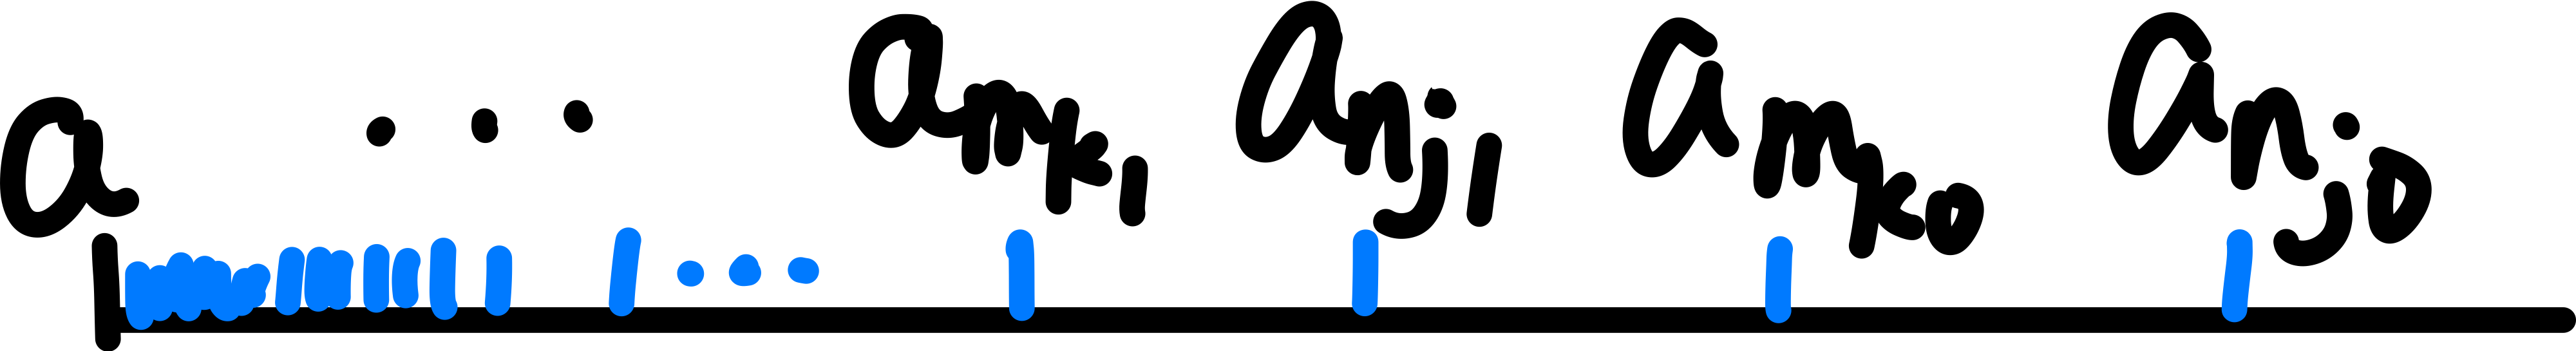
\includegraphics[width=0.5\linewidth]{homework/hw11.assets/image-20250420224142076.png}
    \caption{unbounded total variation by alternating limsup/inf seq}
    \label{fig:unbounded total variation by alternating limsup/inf seq}
\end{figure}
Thus, by picking $j_0 = \max (N_1,N_2)$, we can pick $k_0$ s.t. $ a_{m_{k_0}} < a_{n_{j_0}}$, and then pick $j_1$ s.t. $ a_{m_{j_1}} < a_{n_{k_0}}$ ; and inductively, for the pick of $j_p$, we can always pick $k_p$ s.t. $ a_{m_{k_p}} < a_{n_{j_p}}$ an then pick $ a_{m_{j_{p+1}}} < a_{n_{k_p}}$.\\
We do this process to get the finite seq $j_0,k_0 , j_1,k_1,\cdots, j_p,k_p$ for some int $p$. Then we have: 
\[
T_F ([a,a_{n_{j_0}}]) \geq  |F(a_{n_{j_0}}) - F( a_{m_{k_0}}) |  + |F(a_{n_{k_0}}) - F( a_{m_{j_1}}) | + \cdots + |F(a_{n_{j_p}}) - F( a_{m_{k_p}}) | + |F(a_{n_{k_p}}) - F( a) |  \geq p\frac{\epsilon}{2}
\]
As $p\to \infty$, we have $T_F ([a,a_{j_0}])\geq p\frac{\epsilon}{2} \to\infty$. Thus by def, $T_F ([a,a_{j_0}])  = \infty$, contradicting the assumption that $F$ is a function of bounded variation.\\
Thus by contradiction, it shows that \[
L \leq  l +\epsilon
\]
Since $L \geq l$ and $\epsilon > 0$ is arbitrary, this finishes the proof that \[
L = l
\]
Since we have $\limsup _{x \rightarrow a^{+}} F(x) = \liminf _{x \rightarrow a^{+}} F(x) $, we then have: \[
    \lim_{x\to a+}F(x)  \;\exists
\]
By same reasoning, we can get that \[
  \lim_{x\to a-}F(x)  \;\exists
\]
\end{proof}







\section{$AC  \& L^1$ 函数的导数绝对值的总积分为 $0\implies f = 0$}
  Let $f\colon\mathbb{R}\to \mathbb{R}$ be an absolutely continuous function. Assume that $f\in L^1(\mathbb{R})$,  and that  \[
    \lim_{t\to0+}\int_{-\infty}^\infty\left|\frac{f(x+t)-f(x)}{t}\right|\,dx=0.
  \]
  Prove that $f=0$. \textit{Hint}: consult Fatou Samba but ignore any dance moves.

\begin{proof}
    We define: \[
    D_t(x) : = \frac{f(x+t) -f(x)}{t}
    \]
    Since $f \in AC$, we have that $f'\in L^1(m)$ exists a.e., thus by def of derivative we have: 
    So we take a seq of functions $g_n : = |D_{1/n}|$, we then have: \[
    \lim_{n\to \infty} g_n =   \lim_{t\to 0^+} |D_t| = |f'|\quad  \text{ a.e.}
    \]
    Notice we are given the condition that: \[
    \lim_{t\to 0^+} \| D_t\|_1 =  \lim_{n\to \infty} \int g_n  = 0
    \]
   Since fixing $t$, $f(x+t)$ and $f(x) $ are measurable functions, $D_t$ is also measurable, and thus $g_n \in L^+(m)$ for each $n$. (we can ignore the points where the limit does not exist, since the set of these points has Lebesgue measure $0$.)\\ 
    Applying Fatou's Lemma we have: $$
\int \liminf _{n \rightarrow \infty}g_n\,  d x \leq \liminf _{n \rightarrow \infty} \int g_n d x =  \lim_{n\to \infty} \int g_n  = 0
$$
Since $g_n$ and $\liminf_{n\to \infty} g_n = \lim_{n\to \infty} g_n$ are nonnegative, we have: \[
|f'| =     \lim_{n\to \infty} g_n  = 0 \quad \text{a.e.}
\]
Thus \[
f' = 0\quad \text{a.e.}
\]
Since by AC, we can apply FTC: Let $[a,b]$ be an arbitrary interval, then by FTC we have: \[
f(x)  - f(a) = \int_a^x 0 \, dy = 0,\quad \forall x\in [a,b]
\]
Thus \[
f(x) = f(a) ,\quad \forall x\in [a,b]
\]
Since the interval $[a,b]$ is arbitrary, this proves: $f$ is a constant function. (By taking $I_n : = [-n,n]$ over $n\in\mathbb{N}$, we can get $f(x) = 0$ for all $x\in \mathbb{R}$.)\\
Suppose for contradiction that $f= c \not = 0 $, then \[
\int |f| = \int_{\mathbb{R}} |c|   = \infty
\]contradicting $f \in L^1(m)$, thus we have \[
f = 0
\]This finishes the proof.
\end{proof}







\end{document}